\documentclass[12pt,report]{jsbook}
\usepackage{mymacros}
\usepackage{mymacro}
\usepackage{okumacro}
\usepackage{here}
\setcounter{secnumdepth}{3}
\usepackage{pifont} 

\makeatletter
% \def\@pdfm@dest#1{%
  % \Hy@SaveLastskip
  % \@pdfm@mark{dest (#1) [@thispage /\@pdfview\space @xpos @ypos null]}%
  % \Hy@RestoreLastskip
 % }
\makeatother


\renewcommand{\baselinestretch}{1}
\begin{document}
\pagestyle{empty}

%%%%%%%%%%%%%%%%%%%%%%%%%%%%%%%%%%%%%%%%%%%%%%%%%%%%%%%%%%%%%%%%%%%%%%
%このファイルは論文の表紙です。タイトルや名前等は適宜変更して下さい。
%
%     作者不明   作成日不明(1997年1月既存)
%     宇佐見庄五@内匠研 修正    Wed Jan 14 2004
%%%%%%%%%%%%%%%%%%%%%%%%%%%%%%%%%%%%%%%%%%%%%%%%%%%%%%%%%%%%%%%%%%%%%%
\thispagestyle{empty}
\vspace*{1cm}
{\normalsize 
\begin{center}
{\Large 平成22年度\hspace{1cm}修士論文}\\\vspace{1.5cm}
\huge{\bf トレースログ可視化ツールにおける\\統計情報表示機能}\\
\vspace{6.8cm}
\end{center}

\begin{flushright}
\begin{tabular}{cl}
\\提 出 日   & 平成23年 2月 14日\\\vspace{-1mm}
主査 & 山本 晋一郎 教授\\\vspace{-1mm}
副査 & 戸田 尚宏 教授\\\vspace{-1mm}
副査 & 太田 淳 准教授\\\vspace{-1mm}
所 属     & 愛知県立大学\\\vspace{-1mm}
           & 情報科学研究科\\\vspace{-1mm}
           & 情報システム専攻\\\vspace{-1mm}
学生番号   & 2009834003\\
           & \\
\multicolumn{2}{c}{\Large{市原 大輔}}
\end{tabular}
\end{flushright}
}
\newpage
%%%%%%%%%%%%%%%%%%%%%%%%%%%%%%%%%%%%%%%%%%%%%%%%%%%%%%%%%%%%%%%%%%%%%%%%%%
% 目次
%-------------------------------------------------------------------------
\pagestyle{plain} \pagenumbering{roman}
\setcounter{page}{1}
\setcounter{tocdepth}{2}
\tableofcontents

\clearpage
%%%%%%%%%%%%%%%%%%%%%%%%%%%%%%%%%%%%%%%%%%%%%%%%%%%%%%%%%%%%%%%%%%%%%%%%%%
% 本文
%-------------------------------------------------------------------------
\pagestyle{plain} \pagenumbering{arabic}
\setcounter{page}{1}


\section{TraceLogVisualizerの全体像}

TLVの主機能は,2つの主たるプロセスと6種の外部ファイルによって実現される.
図\ref{fig:tlv}にTLVの全体像を示す.

2つの主たるプロセスとは,標準形式への変換と,図形データの生成である.
標準形式への変換は,任意の形式をもつトレースログを標準形式トレースログに変換する処理である.
この処理には,外部ファイルとして変換元のトレースログファイル,リソースを定義したリソースファイル,リソースタイプを定義したリソースヘッダファイル,標準形式トレースログへの変換ルールを定義した変換ルールファイルが読み込まれる.

また,図形データの生成は,変換した標準形式トレースログに対して可視化ルールを適用し図形データを生成する処理である.
この処理には外部ファイルとして可視化ルールファイルが読み込まれる.
可視化ルールファイルとは図形と可視化ルールの定義を記述したファイルである.

TLVは,トレースログとリソースファイルを読み込み,トレースログの対象に対応したリソースヘッダファイル,変換ルールファイルの定義に従い,標準形式トレースログを生成する.
生成された標準形式トレースログに可視化ルールファイルで定義される可視化ルールを適用し図形データを生成した後,画面に表示する.

生成された標準形式トレースログと図形データは,TLVデータとしてまとめられ可視化表示の元データとして用いられる.
TLVデータはTLVファイルとして外部ファイルに保存することが可能であり,TLVファイルを読み込むことで,標準形式変換と図形データ生成の処理を行わなくても可視化表示できるようになる.

図\ref{fig:TLVscreenshot}に,TLVのスクリーンショットを示す.

\begin{figure}[!t]
\begin{center}
\includegraphics[scale=0.7]{img/tlv.eps}
\caption{TLVの全体像}
\label{fig:tlv}
\end{center}
\end{figure}

\begin{figure}[!t]
\begin{center}
\includegraphics[scale=0.7]{img/TLVscreenshot.eps}
\caption{TLVのスクリーンショット}
\label{fig:TLVscreenshot}
\end{center}
\end{figure}

\subsection{JSON}

リソースファイル,リソースヘッダファイル,変換ルールファイル,可視化ルールファイルは,JSON(JavaScript Object Notation)\cite{JSON}と呼ばれるデータ記述言語を用いて記述する.

JSONは,主にウェブブラウザなどで使用されるECMA-262,revision 3準拠のJavaScript(ECMAScript)と呼ばれるスクリプト言語のオブジェクト表記法をベースとしており,RFC 4627としてで仕様が規定されている.
JSONはUnicodeのテキストデータで構成され,バイナリデータを扱うことはできない.
また,JSONではシンタックスのみの規定がなされ,セマンティクスは規定されていない.

JSONの特徴は,シンタックスが単純であることである.
これは,人間にとっても読み書きし易く,コンピュータにとっても解析し易いことを意味する.
また,複数のプログラミング言語でJSONファイルを扱うライブラリが実装されており,異なる言語間のデータ受け渡しに最適である.
JSONが利用可能なプログラミング言語としては,ActionScript, C, C++, C\#, ColdFusion, Common Lisp, Curl, D言語, Delphi, E, Erlang, Haskell, Java, JavaScript (ECMAScript), Lisp, Lua, ML, Objective CAML, Perl, PHP, Python, Rebol, Ruby, Scala, Squeakなどがある.

TLVの各ファイルのフォーマットにJSONを採用した理由はこれらの特徴による.
シンタックスが単純であることにより,ユーザの記述コスト,習得コストを低減させることができ,また,複数のプログラミング言語でパース可能であることによりファイルに可搬性を持たせることができるからである.

JSONで表現するデータ型は以下のとおりであり,これらを組み合わせることでデータを記述する.
\begin{itemize}
\setlength{\itemsep}{0.5\itemsep}
\item 数値(整数,浮動小数点)
\item 文字列(Unicode)
\item 真偽値(true,false)
\item 配列(順序付きリスト)
\item オブジェクト(ディクショナリ,ハッシュテーブル)
\item null
\end{itemize}

JSONの文法をEBNFと正規表現を用いて説明する.

JSONは,次に示すようにオブジェクトか配列で構成される.

\begin{EBNF}
JSONText = Object | Array;
\end{EBNF}

オブジェクトは複数のメンバをカンマで区切り,中括弧で囲んで表現する.
メンバは名前と値で構成され,名前のあとにはセミコロンが付く.
メンバの名前は値であり,データ型は文字列である.
オブジェクトの定義を次に示す.

\begin{EBNF}
Object = "{",Member,[{",",Member}],"}";
Member = String,":",Value;
\end{EBNF}

配列は複数の値を持つ順序付きリストであり,値をコンマで区切り,角括弧で囲んで表現する.
次に配列の定義を示す.

\begin{EBNF}
Array = "[",Value,[{",",Value}],"]";
\end{EBNF}

値は,文字列,数値,オブジェクト,配列,真偽値,nullのいずれかである.
文字列はダブルクオーテーションで囲まれたUnicode列である.
数値は10進法表記であり,指数表記も可能である.
値の定義を次に示す.

\begin{EBNF}
Value = String|Number|Object|Array|Boolean|"null";
String = /"([^"\]|\n|\"|\\|\b|\f|\r|\t|\u[0-9a-fA-F]{4})*"/;
Boolean = "true"|"false";
Number = ["-"],("0"|Digit1-9,[Digit]),[".",Digit],Exp;
Exp = ["e",[("+"|"-")],Digit];
Digit = /[0-9]+/;
Digit1-9 = /[1-9]/;
\end{EBNF}

表\ref{JSONObject}にJSONにおけるオブジェクトを定義した例を示す.

\begin{FileToPage}{JSONにおけるオブジェクトを定義した例}{JSONObject}
{
  "Image":{
    "Width":  800,
    "Height": 600,
    "Title":  "View from 15th Floor",
    "Thumbnail":{
      "Url":    "http://www.example.com/image/481989943",
      "Height": 125,
      "Width":  "100"
    },
    "IDs": [116, 943, 234, 38793]
  }
}
\end{FileToPage}

表\ref{JSONArray}にJSONにおける配列を定義した例を示す.

\begin{FileToPage}{JSONにおける配列を定義した例}{JSONArray}
[
  {
    "City":      "SAN FRANCISCO",
    "State":     "CA",
    "Zip":       "94107",
    "Country":   "US"
  },
  {
    "City":      "SUNNYVALE",
    "State":     "CA",
    "Zip":       "94085",
    "Country":   "US"
  },
  {
    "City":      "HEMET",
    "State":     "CA",
    "Zip":       "92544",
    "Country":   "US"
  }
]
\end{FileToPage}

\chapter{�g���[�X���O�Ž����c�[��(TLV)}
\section{TLV�ɂ�����ėp���Ɗg����}
TLV�́C�ėp���Ɗg�������������邱�Ƃ�ڕW�Ƃ��Ă���D

�ėp���Ƃ́C�Ž����\���������g���[�X���O�̌`���𐧌����Ȃ����Ƃł���C
�Ž����\���̎d�g�݂��g���[�X���O�̌`���Ɉˑ������Ȃ����Ƃɂ���Ď�����
��D��̓I�ɂ́C�܂��C�g���[�X���O�𒊏ۓI�Ɉ�����悤�ɁC�g���[�X���O
����ʉ������W���`���g���[�X���O���`����D�����āC�C�ӂ̌`���̃g���[
�X���O��W���`���g���[�X���O�ɕϊ�����d�g�݂��C�ϊ����[���Ƃ��Č`����
����D�ϊ����[���̋L�q�ŔC�ӂ̃g���[�X���O���W���`���g���[�X���O�ɕϊ�
���邱�Ƃ��ł��邽�߁C������g���[�X���O�̉Ž����ɑΉ����邱�Ƃ��”\
�ƂȂ�D

�g�����Ƃ́C�g���[�X���O�ɑΉ�����Ž����\�������[�U���x���Ŋg���ł���
���Ƃ�\���C�g���[�X���O����Ž����\�����s���d�g�݂𒊏ۉ����C�������
�������[���Ƃ��Č`�������Ē�`���邱�ƂŎ�������D�Ž������[�����L�q��
�邱�Ƃɂ��C�g���[�X���O���̔C�ӂ̏������R�ȕ\�����@�ʼnŽ������邱
�Ƃ��”\�ɂȂ�D

\section{TraceLogVisualizer�̐݌v}\label{sec:tlv_d}

TLV�̎�@�\�́C2�‚̃v���Z�X��6��̊O���t�@�C���ɂ���Ď��������D
TLV�̑S�̑���}\ref{fig:tlv}�Ɏ����D

2�‚̃v���Z�X�Ƃ́C�W���`���ւ̕ϊ��ƁC�}�`�f�[�^�̐����ł���D�W
���`���ւ̕ϊ��́C�C�ӂ̌`�������ƒg���[�X���O��W���`���g���[�X���O��
�ϊ����鏈���ł���D���̏����ɂ́C�O���t�@�C���Ƃ��ĕϊ����̃g���[�X��
�O�t�@�C���C�W���`���g���[�X���O�ɓo�ꂷ�郊�\�[�X���`�������\�[�X�t�@�C���C
���\�[�X�^�C�v���`��
�����\�[�X�w�b�_�t�@�C���C�W���`���g���[�X���O�ւ̕ϊ����[�����`����
�ϊ����[���t�@�C�����ǂݍ��܂��D

�܂��C�}�`�f�[�^�̐����́C�W���`���g���[�X���O�ɑ΂��āA�Ž������[���ƌĂ�

��K�p���}�`�f�[�^�𐶐����鏈���ł���D���̏����ɂ͊O���t�@�C���Ƃ�
�ĉŽ������[���t�@�C�����ǂݍ��܂��D�Ž������[���t�@�C���Ƃ́C
�}�`�ƉŽ������[���̒�`���L�q�����t�@�C���ł���D

% TLV�́C�g���[�X���O�ƃ��\�[�X�t�@�C����ǂݍ��݁C�g���[�X���O�̑Ώۂɑ�
% ���������\�[�X�w�b�_�t�@�C���C�ϊ����[���t�@�C���̒�`�ɏ]���C�W���`��
% �g���[�X���O�𐶐�����D�������ꂽ�W���`���g���[�X���O�ɉŽ������[���t�@
% �C���Œ�`�����Ž������[����K�p���}�`�f�[�^�𐶐�������C��ʂɕ\��
% ����D

�������ꂽ�W���`���g���[�X���O�Ɛ}�`�f�[�^�́CTLV�f�[�^�Ƃ��Ă܂Ƃ߂��
�Ž����\���̌��f�[�^�Ƃ��ėp������DTLV�f�[�^��TLV�t�@�C���Ƃ��ĊO��
�t�@�C���ɕۑ����邱�Ƃ��”\�ł���CTLV�t�@�C����ǂݍ��ނ��ƂŁC�W���`
���ϊ��Ɛ}�`�f�[�^�����̏������s��Ȃ��Ă��Ž����\���ł���悤�ɂȂ�D

�}\ref{fig:TLVscreenshot}�ɁCTLV�̃X�N���[���V���b�g�������D

\begin{figure}[!t]
\begin{center}
\includegraphics[scale=0.7]{tlv.eps}
\caption{TLV�̑S�̑�}
\label{fig:tlv}
\end{center}
\end{figure}

\begin{figure}[!t]
\begin{center}
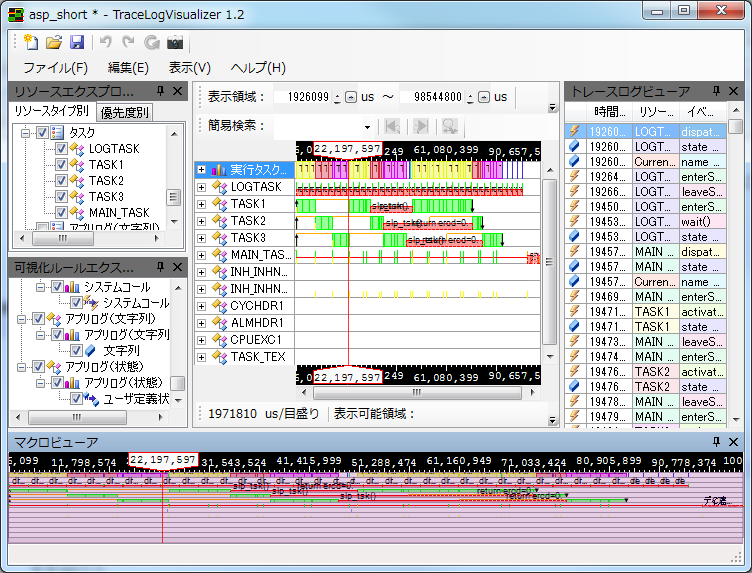
\includegraphics[width=0.7\textwidth]{tlv.png}
\caption{TLV�̃X�N���[���V���b�g}
\label{fig:TLVscreenshot}
\end{center}
\end{figure}


\section{�W���`���g���[�X���O}\label{sec:log}
\subsection{�g���[�X���O�̒��ۉ�}\label{sec:logchushou}
�W���`���g���[�X���O���Ă���ɂ�����C�g���[�X���O�̒��ۉ����s�����D
���ʂ��ȉ��ɂ܂Ƃ߂�D

% �g���[�X���O���C���n��ɃC�x���g���L�^�������̂ł���D
% �C�x���g�Ƃ̓C�x���g�������̑����̕ω��C�C�x���g�������̐U�镑���ƍl��
% ���D�����ŁC�C�x���g�����������\�[�X�ƌď̂��C�ŗL�̎��ʎq�����‚��̂�
% ����D�‚܂�C���\�[�X�Ƃ́C�C�x���g�̔������ł���C���O�������C�ŗL��
% ���������‚��̂ƍl���邱�Ƃ��ł���D

% ���\�[�X�͌^�ɂ�葮���C�U�镑��������t������D�����Ń��\�[�X�̌^��
% ���\�[�X�^�C�v�ƌď̂���D

% �����́C���\�[�X���ŗL�ɂ��•�����C���l�C�^�U�l�ŕ\�����X�J���[�f�[
% �^�Ƃ��C�U�镑���̓��\�[�X�̍s�ׂł���Ƃ���D

% ���\�[�X�^�C�v�ƃ��\�[�X�̊֌W�́C�I�u�W�F�N�g�w���ɂ�����N���X�ƃI�u
% �W�F�N�g�̊֌W�ɗގ����Ă���C�����ƐU�镑���̓����o�ϐ��ƃ��\�b�h�ɗ�
% �����Ă���D�������C�U�镑���̓��\�[�X�̂Ȃ�炩�̍s�ׂ�\�����Ă���C
% ���\�b�h�́C�����o�ϐ��𑀍삷�邽�߂̊֐���葱����\���T�O�Ƃ͈قȂ�D

% ��ɁC�U�镑���́C�����̕ω��𔺂�Ȃ��C�x���g��\�����邽�߂ɗp����D
% �U�镑���͔C�ӂ̐��̃X�J���[�f�[�^�������Ƃ��Ď󂯎�邱�Ƃ��ł��C����
% �́C�}�`�`��̍ۂ̏����C���邢�͕`��ޗ��Ƃ��ėp�����邱�Ƃ�z�肵��
% ����D

%% �}\ref{fig:resourceTypeSample}�Ɛ}\ref{fig:resourceSample}�ɁC���\�[�X
%% �^�C�v�ƃ��\�[�X��}�ŕ\��������������D����ɁC�}
%% \ref{fig:resourceTypeSampleByTask}�ɁCRTOS(Real-time operating system)
%% �ɂ�����^�X�N�̊T�O�����\�[�X�^�C�v�Ƃ��ĕ\����������C�}
%% \ref{fig:resourceSampleByTask}�ɁC���\�[�X�^�C�vTask�̃��\�[�X�̗�Ƃ�
%% ��MainTask�������D

% �g���[�X���O�̒��ۉ����ȉ��ɂ܂Ƃ߂�D

\begin{description}
\item[�g���[�X���O] \mbox{} \\
���n��ɃC�x���g���L�^�������́D
\item[�C�x���g] \mbox{} \\
���\�[�X�̑����̒l�̕ω��C���\�[�X�̐U�镑���D
\item[���\�[�X] \mbox{} \\
�C�x���g�̔������D�ŗL�̖��O�C���������D
\item[���\�[�X�^�C�v] \mbox{} \\
���\�[�X�̌^�D���\�[�X�̑����C�U�镑��������t����D
\item[����] \mbox{} \\
���\�[�X���ŗL�ɂ����D������C���l�C�^�U�l�̂����ꂩ�ŕ\�������X�J���[�f�[�^�ŕ\�����D
\item[�U�镑��] \mbox{} \\
���\�[�X�̍s�ׁD��ɑ����̒l�̕ω��𔺂�Ȃ��s�ׂ��C�x���g�Ƃ��ċL�^���邽�߂ɗp���邱�Ƃ�z�肵�Ă���D
�U�镑���͔C�ӂ̐��̃X�J���[�f�[�^�������Ƃ��Ď󂯎�邱�Ƃ��ł���D
\end{description}

%% \begin{figure}[p]
%% \begin{tabular}{cc}
%% \begin{minipage}{0.5\hsize}
%% \begin{center}
%% \includegraphics[scale=0.5]{resourceTypeSample.eps}
%% \caption{���\�[�X�^�C�v}
%% \label{fig:resourceTypeSample}
%% \end{center}
%% \end{minipage}
%% \begin{minipage}{0.5\hsize}
%% \begin{center}
%% \includegraphics[scale=0.5]{resourceSample.eps}
%% \caption{���\�[�X}
%% \label{fig:resourceSample}
%% \end{center}
%% \end{minipage}
%% \end{tabular}
%% \end{figure}

%% \begin{figure}[p]
%% \begin{tabular}{ccc}
%% \begin{minipage}{0.35\hsize}
%% \begin{center}
%% \includegraphics[scale=0.5]{resourceTypeSampleByTask.eps}
%% \caption{�^�X�N�����\�[�X�^�C�vTask�Ƃ��ĕ\��������}
%% \label{fig:resourceTypeSampleByTask}
%% \end{center}
%% \end{minipage}
%% \begin{minipage}{0.25\hsize}
%% \mbox{}\\
%% \end{minipage}
%% \begin{minipage}{0.3\hsize}
%% \begin{center}
%% \includegraphics[scale=0.5]{resourceSampleByTask.eps}
%% \caption{���\�[�X�^�C�vTask�̃��\�[�XMainTask�̗�}
%% \label{fig:resourceSampleByTask}
%% \end{center}
%% \end{minipage}
%% \end{tabular}
%% \end{figure}

\subsection{�W���`���g���[�X���O�̒�`}

�{���߂ł́C�O���߂Œ��ۉ������g���[�X���O���C�W���`���g���[�X���O�Ƃ�
�Č`��������D�W���`���g���[�X���O�̒�`�́CEBNF(Extended Backus Naur
Form)����яI�[�L���Ƃ��Đ��K�\����p���čs���D���K�\���̓X���b�V���L��
({\tt /})�ŋ��ނ��̂Ƃ���D

�O���߂ɂ��΁C�g���[�X���O�́C���n��ɃC�x���g���L�^�������̂ł����
�ŁC�P�‚̃��O�ɂ͎����ƃC�x���g���܂܂��ׂ��ł���D�g���[�X���O���L
�^���ꂽ�t�@�C���̃f�[�^��\verb|TraceLog|�C\verb|TraceLog|�����s�L����
��؂����P�s��\verb|TraceLogLine|�Ƃ���ƁC�����͎���EBNF�ŕ\�������D

\begin{EBNF}
TraceLog = { TraceLogLine,"\n" };
TraceLogLine = "[",Time,"]",Event;
\end{EBNF}

\verb|TraceLogLine|��"\verb|[|","\verb|]|"�Ŏ������͂݁C���̌��ɃC�x���g���L�q������̂Ƃ���D

������\verb|Time|�Ƃ��Ē�`����C���Ɏ����悤�ɐ��l�ƃA���t�@�x�b�g�ō\��������̂Ƃ���D

\begin{EBNF}
Time = /[0-9a-Z]+/;
\end{EBNF}

�A���t�@�x�b�g���܂܂��̂́C10�i���ȊO�̎�����\���ł���悤�ɂ��邽
�߂ł���D����́C�����̒P�ʂƂ��āu�b�v�ȊO�̂��́C���Ƃ��΁u���s����
  ���v�Ȃǂ�\���ł���悤�ɍl���������߂ł���D���̒�`����C�����ɂ́C
2�i������36�i���܂ł��w��ł��邱�Ƃ��킩��D

�O���߂ɂāC�C�x���g���C���\�[�X�̑����̒l�̕ω��C���\�[�X�̐U�镑����
���ۉ������D���̂��߁C�C�x���g�����̂悤�ɒ�`�����D

\begin{EBNF}
Event = Resource,".",(AttributeChange|BehaviorHappen);
\end{EBNF}

{\tt Resource}�̓��\�[�X��\���C{\tt AttributeChange}�͑����̒l�̕ω��C
�x���g�C{\tt BehaviorHappen}�͐U�镑���C�x���g��\���D���\�[�X�̓��\�[
�X���ɂ�钼�ڎw��C���邢�̓��\�[�X�^�C�v���Ƒ��������ɂ������w���
2�ʂ�̎w����@��p�ӂ����D

���\�[�X�̒�`�����Ɏ����D

\begin{EBNF}
Resource = ResourceName
         | ResourceTypeName,"(",AttributeCondition,")";
ResourceName = Name;
ResourceTypeName = Name;
Name = /[0-9a-Z_]+/;
\end{EBNF}

���\�[�X�ƃ��\�[�X�^�C�v�̖��O�͐��l�ƃA���t�@�x�b�g�C�A���_�[�o�[�ō\�������Ƃ����D
{\tt AttributeCondition}�͑��������w��L�q�ł���D
����͎��̂悤�ɒ�`����D

\begin{EBNF}
AttributeCondition = BooleanExpression;
BooleanExpression = Boolean
   |ComparisonExpression
   |BooleanExpression,[{LogicalOpe,BooleanExpression}]
   |"(",BooleanExpression,")";
Boolean = "true"|"false";
ComparisonExpression = AttributeName,ComparisonOpe,Value;
LogicalOpe = "&&"|"||";
ComparisonOpe = "=="|"!="|"<"|">"|"<="|">=";
\end{EBNF}

���������w��́C�_�����ŕ\����C����Ƃ��đ����̒l�̏��������C�������Z�q���r���Z�q��p���ċL�q�ł���Ƃ����D

{\tt AttributeName}�͑����̖��O�ł���C���\�[�X���⃊�\�[�X�^�C�v���Ɠ��l�ɁC���̂悤�ɒ�`����D

\begin{EBNF}
AttributeName = Name;
\end{EBNF}

�C�x���g�̒�`�ɂāC\verb|AttributeChange|�͑����̒l�̕ω��C\verb|BehaviorHappen|�͐U�镑���Ƃ����D
�����́C���\�[�X�ƃh�b�g"\verb|.|"�ł‚Ȃ��邱�Ƃł��̃��\�[�X�ŗL�̂��̂ł��邱�Ƃ������D
���\�[�X�̑����̒l�̕ω��ƐU�镑���͎��̂悤�ɒ�`�����D
\newpage
\begin{figure}[h]
\begin{EBNF}
AttributeChange = AttributeName,"=",Value;
Value = /[^"\\]+/;
BehaviorHappen =  BehaviorName,"(",Arguments,")";
BehaviorName = Name;
Arguments = [{Argument,[","]}];
Argument = /[^"\\]*/;
\end{EBNF}
\end{figure}

�����̕ω��C�x���g�́C�������ƕω���̒l�������Z�q�ł‚Ȃ����ƂŋL�q���C�U�镑���C�x���g�́C�U�镑�����ɑ����ăJ���}�ŋ�؂�������������"{\tt ()}"�ň͂݋L�q����Ƃ����D


\subsection{�W���`���g���[�X���O�̗�}

�W���`���g���[�X���O�̒�`�����ɋL�q�����C�W���`���g���[�X���O�̗��}\ref{standartFormatTraceLogSample}�Ɏ����D

\begin{figure}[h]
\begin{lstlisting}
[2403010]MAIN_TASK.leaveSVC(ena_tex,ercd=0)
[4496099]MAIN_TASK.state=READY
[4496802]TASK(state==RUNNING).state=READY
\end{lstlisting}
\caption{�W���`���g���[�X���O�̗�}
\label{standartFormatTraceLogSample}
\end{figure}

1�s�ڂ����\�[�X�̐U�镑���C�x���g�ł���C2�s�ځC3�s�ڂ������̒l�̕ω��C�x���g�ł���D
1�s�ڂ̐U�镑���C�x���g�ɂ͈������w�肳��Ă���D

1�s�ځC2�s�ڂ̓��\�[�X�𖼑O�Œ��ڎw�肵�Ă��邪�C3�s�ڂ̓��\�[�X�^�C�v�Ƒ����̏����ɂ���ă��\�[�X����肵�Ă���D

% \section{�}�`�f�[�^}\label{subsec:visualization}
% \subsection{���W�n}

% �}�`���`������W�n�ƁC�\��������W�n�͕������čl����Ƃ���D
% ����ɂ��C�}�`��\���‹�����Ɨ����Ē�`���邱�Ƃ��”\�ɂȂ�D
% �}�`���`������W�n�����[�J�����W�n�C�\��������W�n���f�o�C�X���W�n�ƌď̂���D

% �܂��CTLV�ł́C�����Ǝ��Ԃ������Ɏ��C���[���h���W�n�Ƃ������W�n�𓱓�
% �����D���[�J�����W�n�Œ�`���ꂽ�}�`�́C�͂��߂ɁC���[���h���W�n�ɂ���
% ��C�}�`��\�����ׂ����Ԃ̗̈�Ƀ}�b�s���O����C�����\���‹��Ɉˑ���
% ��f�o�C�X���W�n�Ƀ}�b�s���O���邱�Ƃŕ\������D����ɂ��C�}�`�̕\��
% �̈���C���ۓx�̍��������Ŏw�肷�邱�Ƃ��”\�ɂȂ�D�����ŁC���[�J����
% �W�n���烏�[���h���W�n�ւ̃}�b�s���O�����[���h�ϊ��ƌď̂���D�܂��C�\
% �����鎞�Ԃ̗̈��\�����Ԃƌď̂���D�\�����Ԃ͊J�n�����ƏI�������ŕ\
% ����鎞���̃y�A�ł���D

% ���[�J�����W�n�ɂ����āC�}�`�̑傫���ƈʒu���`����ۂ́Cpixel�P�ʂɂ�
% ���Ύw�肩�C���[���h���W�n�ւ̃}�b�s���O�̈�ɑ΂��銄����\%�Ŏw�肷
% �鑊�Ύw�肩�̂����ꂩ��p����D

% �}\ref{fig:coordinate}�ɍ��W�n�̗���C�}\ref{fig:worldTransform}�Ƀ��[
% ���h�ϊ��̗�������D

% \begin{figure}[tb]
% \begin{center}
% \includegraphics[scale=0.75]{coordinate.eps}
% \caption{���W�n}
% \label{fig:coordinate}
% \end{center}
% \end{figure}

% \begin{figure}[tb]
% \begin{center}
% \includegraphics[scale=0.75]{worldTransform.eps}
% \caption{���[���h�ϊ�}
% \label{fig:worldTransform}
% \end{center}
% \end{figure}

% \subsection{��{�}�`�Ɛ}�`�C�}�`�Q}\label{sec:shape}
% �Ž����\���́C�����̐}�`��g�ݍ��킹�邱�ƂŎ�������D
% ���̍ہC��{�ƂȂ�}�`�̒P�ʂ���{�}�`�ƌď̂���D

% ��{�}�`�Ƃ��Ĉ�����`��͑ȉ~�C���p�`�C�l�p�`�C�����C���C��`�C�������7��ނƂ���D
% ��{�}�`�́C�`���傫���C�ʒu�C�h��‚Ԃ��̐F�C���̐F�C����C�����x�Ȃǂ̑������w�肵�Ē�`����D

% �����̊�{�}�`�����z�I��z�������ɊK�w�I�ɏd�˂����̂��C�P�ɐ}�`�ƌď̂��C�Ž����\���̍ŏ��P�ʂƂ���D
% �}�`�́C�\�������{�}�`�������t���Ŏw�肵�C���O���‚��Ē�`����D
% �}�`�͖��O��p���ĎQ�Ƃ��邱�Ƃ��ł��C���̍ۂɈ�����^���邱�Ƃ��ł���Ƃ���D
% ���̍ہC�����́C�}�`���\�������{�}�`�́C�C�ӂ̑����Ɋ��蓖�Ă邱�Ƃ�z�肵�Ă���D

% �����̐}�`�����z�I��z�������ɊK�w�I�ɏd�˂����̂�}�`�Q�ƌď̂���D
% �}\ref{fig:shapes}�ɐ}�`�Ɛ}�`�Q�̗�������D

% \begin{figure}[tb]
% \begin{center}
% \includegraphics[scale=0.75]{shapes.eps}
% \caption{�}�`�Ɛ}�`�Q}
% \label{fig:shapes}
% \end{center}
% \end{figure}

% \section{�}�`�f�[�^�ƃC�x���g�̑Ή�}

% �{���߂ł́C�O���߂ŏq�ׂ��Ž����\���ƃg���[�X���O�̃C�x���g���ǂ̂悤�ɑΉ��t����̂����q�ׂ�D

% \subsection{�J�n�C�x���g�C�I���C�x���g�C�C�x���g����}
% �O���߂ɂ����āC�Ž����\���́C�}�`�����[���h�ϊ����o�ĕ\�����ԂɃ}�b�s
% ���O���邱�Ƃł��邱�Ƃ���������D�����ŁC�\�����Ԃ̊J�n�����C�I������
% ���C�C�x���g��p���Ďw�肷��Ƃ���D�‚܂�C�w�肳�ꂽ�C�x���g��������
% �鎞�����g���[�X���O��蒊�o���邱�Ƃɂ��\�����Ԃ����肷��D���̂悤
% �ɂ��āC�g���[�X���O�̃C�x���g�ƉŽ����\����Ή��t����D�����ŁC�J�n��
% ���ɑΉ�����C�x���g���J�n�C�x���g�C�I�������ɑΉ�����C�x���g���I���C
% �x���g�ƌď̂��C�\�����Ԃ��C�x���g�ŕ\���������̂��C�x���g���Ԃƌď̂�
% ��D

% \subsection{�Ž������[��}

% �}�`�Q�ƁC���̃}�b�s���O�Ώۂł���C�x���g���Ԃ��\���v�f�Ƃ��Ă��\���̂��C�Ž������[���ƌď̂���D
% �}\ref{fig:timeShape}�ɁC�W���`���g���[�X���O��p���ăC�x���g���Ԃ��`�����Ž������[���̗�������D
% \begin{figure}[tb]
% \begin{center}
% \includegraphics[scale=0.9]{timeShape.eps}
% \caption{�Ž������[��}
% \label{fig:timeShape}
% \end{center}
% \end{figure}
% �}\ref{fig:timeShape}�ɂ����āCrunningShape���C�ʒu�����[�J�����W�̌��_�C
% �傫�������[���h���W�n�̃}�b�s���O�̈�ɑ΂��ĉ���100\%�C�c��80\%�̒���
% �`�ŐF���ΐF�̐}�`�Ƃ���D���̐}�`���C�J�n�C�x���g
% \verb|MAIN_TASK.state=RUNNING|�C�I���C�x���g\verb|MAIN_TASK.state|�Ƃ�
% ��C�x���g���Ԃŕ\������悤��`�������̂��Ž������[��
% taskBecomeRunning�ł���D�J�n�C�x���g\verb|MAIN_TASK.state=RUNNING|�́C
% ���\�[�X\verb|MAIN_TASK|�̑���\verb|state|�̒l��\verb|RUNNING|�ɂȂ���
% ���Ƃ�\���C�I���C�x���g\verb|MAIN_TASK.state|�́C���\�[�X
% \verb|MAIN_TASK|�̑���\verb|state|�̒l���P�ɕς�������Ƃ�\���Ă���D

% taskBecomeRunning���C�}\ref{eventTime}�Ɏ����g���[�X���O����C�x���g��
% ���o���ĕ\�����Ԃ̎��������肵�C�}�`�̃��[���h�ϊ����s�������ʂ��}
% \ref{fig:timeShape}�̉E���Ɏ������̂ł���D

% \begin{lstlisting}[caption=�C�x���g���Ԃ𒊏o����g���[�X���O,label=eventTime]
% [1000]MAIN_TASK.state=RUNNING
% [1100]MAIN_TASK.state=WAITING
% \end{lstlisting}


\subsection{JSON}

���\�[�X�t�@�C���C���\�[�X�w�b�_�t�@�C���C�ϊ����[���t�@�C���C�Ž������[���t�@�C���́CJSON(JavaScript Object Notation)\cite{JSON}�ƌĂ΂��f�[�^�L�q�����p���ċL�q����D

JSON�́C��ɃE�F�u�u���E�U�ȂǂŎg�p�����ECMA-262�Crevision 3������JavaScript�iECMAScript�j�ƌĂ΂��X�N���v�g����̃I�u�W�F�N�g�\�L�@���x�[�X�Ƃ��Ă���CRFC 4627�Ƃ��Ďd�l���K�肳��Ă���D
JSON��Unicode�̃e�L�X�g�f�[�^�ō\������C�o�C�i���f�[�^���������Ƃ͂ł��Ȃ��D
�܂��CJSON�ł̓V���^�b�N�X�݂̂̋K�肪�Ȃ���C�Z�}���e�B�N�X�͋K�肳��Ă��Ȃ��D

JSON�̓����́C�V���^�b�N�X���P���ł��邱�Ƃł���D
����́C�l�ԂɂƂ��Ă��ǂݏ������Ղ��C�R���s���[�^�ɂƂ��Ă���͂��Ղ����Ƃ��Ӗ�����D
�܂��C�����̃v���O���~���O�����JSON�t�@�C�����������C�u��������������Ă���C�قȂ錾��Ԃ̃f�[�^�󂯓n���ɍœK�ł���D
JSON�����p�”\�ȃv���O���~���O����Ƃ��ẮCActionScript, C, C++, C\#, ColdFusion, Common Lisp, Curl, D, Delphi, E, Erlang, Haskell, Java, JavaScript (ECMAScript), Lisp, Lua, ML, Objective CAML, Perl, PHP, Python, Rebol, Ruby, Scala, Squeak�Ȃǂ�����D

TLV�̊e�t�@�C���̃t�H�[�}�b�g��JSON���̗p�������R�͂����̓����ɂ��D
�V���^�b�N�X���P���ł��邱�Ƃɂ��C���[�U�̋L�q�R�X�g�C�K���R�X�g��ጸ�����邱�Ƃ��ł��C�܂��C�����̃v���O���~���O����Ńp�[�X�”\�ł��邱�Ƃɂ��t�@�C���ɉ”������������邱�Ƃ��ł��邩��ł���D

JSON�ŕ\������f�[�^�^�͈ȉ��̂Ƃ���ł���C������g�ݍ��킹�邱�ƂŃf�[�^���L�q����D
\begin{itemize}
\setlength{\itemsep}{0.5\itemsep}
\item ���l(�����C���������_)
\item ������(Unicode)
\item �^�U�l(true�Cfalse)
\item �z��(�����t�����X�g)
\item �I�u�W�F�N�g(�f�B�N�V���i���C�n�b�V���e�[�u��)
\item null
\end{itemize}

JSON�̕��@��EBNF�Ɛ��K�\����p���Đ�������D

JSON�́C���Ɏ����悤�ɃI�u�W�F�N�g���z��ō\�������D

\begin{EBNF}
JSONText = Object | Array;
\end{EBNF}

�I�u�W�F�N�g�͕����̃����o���J���}�ŋ�؂�C�����ʂň͂�ŕ\������D
�����o�͖��O�ƒl�ō\������C���O�ƒl�̓Z�~�R�����ŋ�؂���D
�����o�̖��O�͒l�ł���C�f�[�^�^�͕�����ł���D
�I�u�W�F�N�g�̒�`�����Ɏ����D

\begin{EBNF}
Object = "{",Member,[{",",Member}],"}";
Member = String,":",Value;
\end{EBNF}

�z��͕����̒l���������t�����X�g�ł���C�l���R���}�ŋ�؂�C�p���ʂň͂�ŕ\������D
���ɔz��̒�`�������D

\begin{EBNF}
Array = "[",Value,[{",",Value}],"]";
\end{EBNF}

�l�́C������C���l�C�I�u�W�F�N�g�C�z��C�^�U�l�Cnull�̂����ꂩ�ł���D
������̓_�u���N�I�[�e�[�V�����ň͂܂ꂽUnicode��ł���D
���l��10�i�@�\�L�ł���C�w���\�L���”\�ł���D
�l�̒�`�����Ɏ����D

\begin{EBNF}
Value = String|Number|Object|Array|Boolean|"null";
String = /"([^"\]|\n|\"|\\|\b|\f|\r|\t|\u[0-9a-fA-F]{4})*"/;
Boolean = "true"|"false";
Number = ["-"],("0"|Digit1-9,[Digit]),[".",Digit],Exp;
Exp = ["e",[("+"|"-")],Digit];
Digit = /[0-9]+/;
Digit1-9 = /[1-9]/;
\end{EBNF}

�}\ref{JSONObject}��JSON�ɂ�����I�u�W�F�N�g���`������������D

\begin{figure}[h]
\begin{lstlisting}
{
  "Image":{
    "Width":  800,
    "Height": 600,
    "Title":  "View from 15th Floor",
    "Thumbnail":{
      "Url":    "http://www.example.com/image/481989943",
      "Height": 125,
      "Width":  "100"
    },
    "IDs": [116, 943, 234, 38793]
  }
}
\end{lstlisting}
\caption{JSON�ɂ�����I�u�W�F�N�g���`������}
\label{JSONObject}
\end{figure}

�}\ref{JSONArray}��JSON�ɂ�����z����`������������D

\begin{figure}[h]
\begin{lstlisting}
[
  {
    "City":      "SAN FRANCISCO",
    "State":     "CA",
    "Zip":       "94107",
    "Country":   "US"
  },
  {
    "City":      "SUNNYVALE",
    "State":     "CA",
    "Zip":       "94085",
    "Country":   "US"
  },
  {
    "City":      "HEMET",
    "State":     "CA",
    "Zip":       "92544",
    "Country":   "US"
  }
]
\end{lstlisting}
\caption{JSON�ɂ�����z����`������}
\label{JSONArray}
\end{figure}

% \subsection{�W���`���g���[�X���O�ւ̕ϊ�}\label{convertRule}
% �W���`���g���[�X���O�ւ̕ϊ��́C�g���[�X���O�t�@�C����擪����s�P�ʂ�
% �ǂݍ��݁C�ϊ����[���t�@�C���Œ�`�����u�����[���ɏ]���W���`���g���[
% �X���O�ɒu�����Ă������Ƃōs����D

% ���\�[�X�����̑J�ڂɔ����C�x���g��C���̃g���[�X���O�Ɍ���
% ���Ă������₤�C�x���g�ȂǁC���̃g���[�X���O�̏�񂾂��ł͔��f�ł�
% �Ȃ��C�x���g���o�͂���ɂ́C���莞���ɂ�������胊�\�[�X�̗L���₻�̐��C
% ���胊�\�[�X�̑����̒l�Ȃǂ̏����ŏo�͂𐧌�ł���K�v������D���̂��߁C
% TLV�̕ϊ����[���ł́C�u����������̎w��ƁC�����w��̍ۂɗp�������u
% ���}�N����p���Ď擾�ł���d�g�݂�񋟂��Ă���D

% �W���`���g���[�X���O�Ɋ܂܂�郊�\�[�X�́C���\�[�X�t�@�C���Œ�`�����
% ���Ȃ���΂Ȃ�Ȃ��D���\�[�X�t�@�C���ɂ́C�e���\�[�X�ɂ‚��āC���̖��O
% �ƃ��\�[�X�^�C�v�C�K�v�ł���Ίe�����̏����l���`����D
% �܂��C���̍ۂɎg�p
% ����郊�\�[�X�^�C�v�̓��\�[�X�w�b�_�t�@�C���Œ�`����Ă��Ȃ���΂Ȃ�
% �Ȃ��D���\�[�X�w�b�_�t�@�C���ɂ͊e���\�[�X�^�C�v�ɂ‚��āC���̖��O�Ƒ�
% ���C�U�镑���̒�`���L�q����D

% ���\�[�X�w�b�_�C�ϊ����[���C�Ž������[���͉Ž�������^�[�Q�b�g���ɗp�ӂ���D
% ���̍ۂ̃^�[�Q�b�g�̓��\�[�X�t�@�C���ɋL�q����D

% \subsection{�}�`�f�[�^�̐���}\label{visualizeRule}
% �W���`���ϊ��v���Z�X���o�ē���ꂽ�W���`���g���[�X���O�́C�Ž������[��
% ��K�p����}�`�f�[�^�𐶐�����D�����ŁC�}�`�f�[�^�Ƃ́C���[���h�ϊ���
% �s��ꂽ�S�}�`�̃f�[�^���w���D�Ž������[���͉Ž������[���t�@�C���Ƃ���
% �^�����C�K�p����Ž������[���̓��\�[�X�t�@�C���ɋL�q����D

% �}�`�f�[�^�̐������@�́C�W���`���g���[�X���O����s���‰Ž������[���̃C
% �x���g���Ԃƈ�v���邩���f���C��v�����ꍇ�ɂ��̉Ž������[���̕\������
% �����[���h�ϊ���̗̈�Ƃ��č̗p�����[���h�ϊ����邱�Ƃōs����D
\newpage
\section{TraceLogVisualizer�̂��̑��̋@�\}

�{�߂ł́C�W���`���ϊ��ƉŽ����f�[�^�����̑���TLV��������@�\�ɂ‚��ďq�ׂ�D

\subsection{�}�[�J�[}
TLV�ł́C�Ž����\�����Ƀ}�[�J�[�ƌĂԈ���w��̎����ɔz�u���邱�Ƃ��ł���D
���ڂ���ׂ��C�x���g�̔��������Ƀ}�[�J�[��z�u���邱�ƂŁC�Ž����\�����e�̗�����⏕���邱�Ƃ��ł���D


\subsection{�Ž����\�����̐���}

�Ž����\���c�[���ł́C�Ž����\�����𐧌䂷�鑀�쐫���Ž����\���c�[���S�̂̑��쐫�ɑ傫���e�����邽�߁CTLV�ł͏󋵂ɍ��킹�ėl�X�ȑ���Ő�����s����悤�ɂ����D
TLV�ł́C�Ž����\�����̐���Ƃ��āC�\���̈�̊g��k���C�ړ����s�����Ƃ��ł���D
�����̑�����@�Ƃ��āC�L�[�{�[�h�ɂ�鑀��C�}�E�X�ɂ�鑀��C�l�̓��͂ɂ�鑀���3�‚̕��@��񋟂����D

�}�E�X�ɂ�鑀��́C�N���b�N�ɂ�鑀��C�z�C�[���ɂ�鑀��C�I���ɂ�鑀��C�h���b�O�ɂ�鑀�삪����D
�N���b�N�ɂ�鑀��̓J�[�\���𒎊ዾ�J�[�\���ɕύX���Ă���s���D
���N���b�N�ŃJ�[�\���ʒu�𒆐S�Ɋg��C�E�N���b�N�ŏk�����s���D
�܂��C���_�u���N���b�N���s�����ƂŃN���b�N�ӏ������S�ɂȂ�悤�Ɉړ�����D
�z�C�[���ɂ�鑀��́C�R���g���[���L�[�������Ȃ���z�C�[�����邱�Ƃňړ����s���C�V�t�g�L�[�������Ȃ����փz�C�[�����邱�ƂŃJ�[�\���ʒu�𒆐S�Ɋg��C���փz�C�[�����邱�Ƃŏk������D
�I���ɂ�鑀��ł́C�}�E�X����ɂ��̈��I�����C���̗̈悪�\���̈�ɂȂ�悤�Ɋg�傷��D
�h���b�O�ɂ�鑀��́C�\���̈���h���b�O���邱�Ƃŕ\���̈�̈ړ����s���D

�L�[�{�[�h�ɂ�鑀��́C�Ž����\�����ɂ����ĕ����L�[���������Ƃōs���D���L�[�ŕ\���̈�����Ɉړ����C�E�L�[�ʼnE�Ɉړ�����D

�l�̓��͂ɂ�鑀��ł́C���ڍׂȐ�����s�����Ƃ��ł���D
�Ž����\�����̏㕔�ɂ̓c�[���o�[���p�ӂ���Ă���C�����ŕ\���̈�̊J�n�����ƏI�������𒼐ړ��͂��邱�Ƃ��ł���D

\subsection{�}�N���\��}

TLV�̗v�����͂��s�����ہC�Ž����\�����Ŋg�債���ꍇ�ɑS�̂̓��ǂ̗̈��\�����Ă���̂���m�肽���Ƃ����v�����������D
���̂��߁CTLV�ł́C�}�N���r���[�A�Ƃ����E�B���h�E�����������D

�}�N���r���[�A�ł́C�g���[�X���O�Ɋ܂܂��C�x���g�̍ŏ���������ő厞���܂ł���ɉŽ����\�����Ă���E�B���h�E�ŁC�Ž����\�����ŕ\�����Ă��鎞�Ԃ𔼓����̐F�œh��‚Ԃ��ĕ\������D
�h��‚Ԃ��̈�̃T�C�Y���}�E�X�ŕύX���邱�Ƃ��ł��C����ɑΉ����ĉŽ����\�����̕\���̈��ύX���邱�Ƃ��ł���D

�}�N���r���[�A�ł͉Ž����\�����Ɠ����悤�ɁC�L�[�{�[�h�C�}�E�X�ɂ��C�Ž����\�����̕\���̈���g��k���C�ړ��̐�����s�����Ƃ��ł���D

\subsection{�g���[�X���O�̃e�L�X�g�\��}

TLV�ł́C�W���`���g���[�X���O���e�L�X�g�ŕ\������E�B���h�E�����������D
�����ł́C�g���[�X���O�̓��e���m�F���邱�Ƃ��ł���D

�Ž����\�����ƃe�L�X�g�\���E�B���h�E�͘A�g���Ă���C�e�L�X�g�\���E�B���h�E��ŃJ�[�\�����ړ�������ƁC�J�[�\���ʒu�ɂ���g���[�X���O�̎����ɂ��킹�ĉŽ����\�����̃J�[�\�����\�����ꂽ��C�_�u���N���b�N���邱�ƂőΉ����鎞���ɉŽ����\�������ړ����邱�Ƃ��ł���D
�܂��C�Ž����\�����Ń_�u���N���b�N���邱�ƂŁC�_�u���N���b�N�ʒu�ɂ���}�`�ɑΉ������g���[�X���O���C�e�L�X�g�\���E�B���h�E�̐擪�ɕ\�������悤�ɂȂ��Ă���D

\subsection{�Ž����\�����ڂ̕\��/��\���؂�ւ�}

TLV�ł́C�Ž����\�����鍀�ڂ��Ž������[���P�ʁC���\�[�X�P�ʂŐ؂�ւ��邱�Ƃ��ł���D
���̑���́C���\�[�X�E�B���h�E�ƉŽ������[���E�B���h�E�ōs���D
���\�[�X�E�B���h�E�ł́C���\�[�X�t�@�C���Œ�`���ꂽ���\�[�X���C���\�[�X�^�C�v��O���[�v���”\�ȑ������Ƀc���[�r���[�`���ŕ\�����Ă���C�`�F�b�N�̗L���Ń��\�[�X���ɕ\���̐؂�ւ����s���D
�����悤�ɁC�Ž������[���E�B���h�E�ł́C�Ž������[�����Ƃɕ\���̐؂�ւ����s����D

\subsection{�X�N���v�g�g���@�\}
�W���`���g���[�X���O�ւ̕ϊ������C�}�`�����������C�O���X�N���v�g�ōs����悤�ɂ��邱�ƂŁC
�ϊ��E�Ž������[���ł͋L�q�ł��Ȃ����G�ȉŽ�������������D

�܂��CTLV�ł����Ƃ��������Ԃ�v����ϊ������́C�ϊ����[���ɂ�鏈�����O���X�N���v�g�ɂ�鏈���̕��������ł���ꍇ������D

\subsection{�A�v�����O�@�\}
�A�v���P�[�V�����ɂ�����C������printf�f�o�b�O���s�����߂̋@�\�ł���D
����ɂ��Cprintf�f�o�b�O�ɂ��o�͂�TLV�̃^�C�����C����ɕ\�������邱�Ƃɂ���āC
���b�Z�[�W���o�͂��ꂽ���̃^�X�N��ԓ�����ڂł킩��悤�ɂȂ�D

\subsection{�����[�h�@�\}
�ϊ����[���E�Ž������[�����L�q����ۂɁC
�L�q��ύX���邽�тɃg���[�X���O���J�������K�v������s�ւł���C�Ƃ����v�]���������D

�����ŁC���݊J���Ă���g���[�X���O���ēx�C�ϊ��E�Ž������s�Ȃ������[�h�@�\��lj������D


\section{��3��OJL�Œlj������@�\}
��3��OJL�Œlj������@�\�ɂ‚��ďq�ׂ�D

\subsection{���v���\���@�\}
���[�U����C�u���v���́C���ɒ����Ԃ̃g���[�X���O�ɂ����āC�ǂ̃R�A�ŃA�C�h���������̂��Ȃǂ̉�͂ɖ𗧂‚̂ŁC
���v���𐶐����ăO���t�\������@�\���ق����v�Ƃ����v�]���������D

�����ŁC���v���̐������@�Ǝ����x���Ȃǂ̃O���t�̐ݒ���w�肷�邱�ƂŁC���v���𐶐����ăO���t�\��
����@�\�����������D

�ڍׂ́C\ref{ch:sd}�͂ŏq�ׂ�D


\section{���p����}
���É���w��w�@���Ȋw�����ȕ����g���݃V�X�e�������Z���^�[(NCES)
\footnote{http://www.nces.is.nagoya-u.ac.jp/}����
7���̃v���W�F�N�g�̂����C2���̃v���W�F�N�g�ɂ���ė��p����Ă���D
�܂��C��NCES�̃R���\�[�V�A���^���������ɂ����Ă����p����Ă���D
\section{�ߋ��̎���}
\subsection{�J���v���Z�X}
TLV�́COJL�̊J���e�[�}�Ƃ��ĊJ�����ꂽ�D
% OJL�Ƃ́C
% ��Ƃōs���Ă���\�t�g�E�F�A�J���v���W�F�N�g�����ނƂ�����H����ł�
% ��C���i���x���̎��V�X�e���̊J����ʂ��đn���I�Ȏv�l�͂�g�ɂ‚���Ƃ�
% ���ɁC�P�Ȃ���ɂƂǂ܂�Ȃ������̊J����Ƃ�S�����Ƃɂ��C�[���C�\
% �Z�Ƃ��������Љ�̐���𓥂܂����\�t�g�E�F�A�J���̎��ۂɂ‚��Ċw�Ԃ���
% ��ړI�Ƃ��Ă���D

TLV�̓v���W�F�N�g�x�[�X�ŊJ�����s���C�O�N�x�܂ł͊�Əo�g��1���Ƌ���2����
�v���W�F�N�g�}�l�[�W���𖱂߁C�w���݌v3�����J���������s���Ă����D�i����
�񍐂́C�T��1�x�̃~�[�e�B���O�ƏT��̒�o�ɂ��s�����D

\subsection{�t�F�[�Y����}
TLV�̊J���͕����t�F�[�Y�ɕ������čs���Ă���D�t�F�[�Y1,2,3�͎��OJL1������
����Ď��{���ꂽ�D�t�F�[�Y3,4,5�͎��OJL2�����ɂ���Ď�
�{���ꂽ�D�{�񍐏��ł̓t�F�[�Y5�ȍ~�ɂ‚��ďq�ׂ�D

��3��OJL�ȑO�̃t�F�[�Y�̓��e�͎��ɏq�ׂ�D

\subsubsection{�t�F�[�Y1,2,3}
2007�N5���`2008�N3���܂łɁCOJL1�����ɂ���Ď��{����CTLV�̎�v�@�\
�̎������s��ꂽ\cite{goto}�D

\subsubsection{�t�F�[�Y3,4,5}
2008�N10���`2010�N3���܂łɁCOJL2�����ɂ���Ď��{���ꂽ\cite{mz,dm}�D
��Ȏ��{���e�����Ɏ����D

\begin{itemize}
\item �P�̃e�X�g����уV�X�e���e�X�g
\item �v���̎��W�ƑΉ�
\item TLV 1.0��TOPPERS\cite{TOPPERS}����ւ̌��J�̌�CTLV 1.1����ʌ����Ɍ��J
\item ���t�@�N�^�����O���j�̌���
\end{itemize}


\chapter{TLV�ɑ΂���v��}
\section{���[�U�~�[�e�B���O�ł̗v�����W}
TLV�́C���݁C��{�I�ȋ@�\���������C�@�\�lj�����ѕێ�̒i�K�ɂ���D
����āCTLV���J������ɂ�����C���[�U�~�[�e�B���O���J�Â��C
TLV�ɑ΂���v�������W�����D���W�����v���̒��ł��C
�uCPU���p���Ȃǂ̓��v���̃O���t�\���v����сuTLV�̍������v�́C�ߋ��ɂ��v��
���������̂ŁC�����ɑΉ����邱�Ƃɂ����D



\section{CPU���p���Ȃǂ̓��v���̃O���t�\��} \label{sec:sd_y}
���v���Ƃ́C�f�[�^�𒲍����āC���̃f�[�^�����“����𐔗ʓI�ɕ\�������̂ł���D
�g���[�X���O�̉�͂ɂ����Ă��C���v���͗L�p�ł���D
�Ⴆ�΁C���[�U�����߂�}���`�v���Z�b�T�Ή�RTOS�̃g���[�X���O�ɂ�����
���v���́C���̂悤�Ȃ��̂�����D

\begin{itemize}
\item �^�X�N��CPU���p��
\item �eCPU�̃A�C�h������
\item �C�x���g��
\item �^�X�N�̎��s��
\item �v���G���v�g��
\item �f�B�X�p�b�`��
\item �^�X�N�����s�”\��ԂɂȂ��Ă�����s��ԂɂȂ�܂ł̎���
\item �f�b�h���C���~�X��
\item �f�b�h���C���܂ł̎���
\end{itemize}

�����̓��v���ɂ‚��āC���߂��闝�R�������‚��Љ��D
�Ⴆ�΁C�eCPU�̃A�C�h�����Ԃ́C�}���`�v���Z�b�T�‹��Ő�����CPU���̃A�C�h�����Ԃ̕΂�
�𔭌��ł��C�eCPU�ւ̃^�X�N���蓖�Ă������悭�s���Ă��邩�m���߂邱�Ƃ��ł���D�܂��C
�f�b�h���C���~�X�񐔂́C���Ԑ���̋���RTOS�ɂ����āC�^�X�N�̊��������ł���f�b
�h���C�����I�[�o�[���邱�Ƃ͋�����Ȃ��̂Ń`�F�b�N����K�v������D

�����������v���́C�����̏ꍇ�C�O���t�Ƃ��ĕ\������D�������邱�ƂŁC���v����
���ƂƂȂ�f�[�^�̗l�X�ȓ��������o�I�ɓǂݎ���悤�ɂȂ�D

�������C�����TLV�ł́C�g���[�X���O�̓��v�����������Ƃ͂ł��Ȃ��D�Ȃ��Ȃ�C
�����TLV�������f�[�^�́C�g���[�X���O�Ƃ������n���񂾂���ł���D
���v���������c�[�����Ȃ��ꍇ�C���̂悤�Ȗ�肪����D

�܂��C���v���𓾂�R�X�g���傫���D���[�U�́C�Ž������ꂽ�g���[�X���O�����ƂŐ�����K�v������C�܂��C���̍�Ƃ͌����Ƃ����傢�ɍl�����C���m���Ɍ�����D
���Ƃɂ�铝�v���̎擾��
���ɁC�X�N���v�g�𗘗p������@������D���̕��@�́C�X�N���v�g�̊J���R�X�g�͂�������̂́C�J����͎��Ƃ�����ƃR�X�g��}�����C���m�������シ��D�������Ȃ���CTLV��p������͍�ƒ��ɁC��������Ԃɂ����铝�v��񂪕K�v�ɂȂ����ꍇ�CTLV�ȊO�̃A�v���P�[�V�����ɖړI�̋�ԏ�����͂��Ď��s����K�v������D�܂��C���v�����O���t�����邽�߂ɃO���t�쐬�c�[���̗��p���l������D���̂悤�ɁC�X�N���v�g�𗘗p������@�ł́C�����̃A�v���P�[�V�����𗘗p����K�v������̂ŁC��͍�Ƃ�������ł���D

���������āC��R�X�g�ŐM�����̍������v���𓾂��C�܂��C��Ƃ������I�ɍs��
��悤�C���v���𓾂ăO���t�Ƃ��ĕ\������@�\�����߂�ꂽ�D
�����ʼn�X�́C�����̗v������������@�\�𓝌v���\���@�\�Ɩ��t���Ď��������D
���̋@�\�ɂ‚��āC\ref{ch:sd}�͂Ő�������D

\section{TLV�̍�����}
TLV�́C�g���[�X���O�̉Ž����Ɏ��Ԃ�������D�Ⴆ�΁C��7,000�s\footnote{�v���Z�b�T��2�—��p�����V�X�e���ŁC�}���`�v���Z�b�T�Ή�RTOS�ł���TOPPERS/FMP�J�[�l��\cite{fmp}����252�b�̊Ԃɏo�͂����s���ł���D}�̃g���[�X���O�ɑ΂��Ė�3���̎��Ԃ�v����D��50,000�s�̃g���[�X���O�ɑ΂��ẮC10���Ԉȏ�Ƃ������p�ɑς��Ȃ����Ԃ�v�����C�Ƃ����񍐂�����D

���̖��ɑ΂��āCOJL2�������������s����\cite{mz}�D���ʁC���G�ȏ������s�����\�b�h�����݂��Ă���C�\�[�X�R�[�h�𕡎G�������Ă������Ƃ����������D���̂悤�ȏ󋵂ł́C�ێ�⍂����������̂ŁC���t�@�N�^�����O�����邱�ƂɂȂ����D

���ƂȂ��Ă���̂́C�W���`���g���[�X���O�̃p�[�V���O�ɂ����鐳�K�\���̑��p�ƉŽ������[���ɂ�����ÖٓI�Ȗ؍\���ł���D

�܂��C�O�҂ɂ‚��Đ�������D���K�\���́C������̃}�b�`���O���_��ɍs���邪�C�ǂ̂悤�ȕ�������}�b�`���O����̂���ǂ���R�X�g��v����D���̂��߁C���K�\���𑽗p����ƁC�R�[�h�̉“ǐ����ቺ����D

���ɁC��҂ɂ‚��Đ�������D�Ž������[����\������N���X�Q�̒��ɁC�T�O�I�ɖ؍\���ƂȂ�N���X�����邪�C�N���X�݌v����Ė؍\���ŕ\������Ă��Ȃ��D���̂��߁C�؍\�����g���o�[�X���邽�߂̃R�[�h�������̏ꏊ�ɑ��݂��邱�ƂɂȂ�C�ێ琫�Ɖ“ǐ����ቺ���Ă���D

���K�\���́C�W���`���g���[�X���O��\���N���X�ő��p����Ă���D���̃N���X�́CTLV�̏����ő��p�����̂ŁC���̖����ɉ������邱�Ƃɂ����D���̃��t�@�N�^�����O�ɂ‚��āC\ref{ch:refact}�͂Ő�������D
\chapter{���v���\���@�\}\label{ch:sd}
\section{�T�v}
���v���\���@�\�́C�g���[�X���O�Ȃǂ̏�񂩂瓝�v���𓾂āC������O���t�Ƃ��ĕ\������@�\�ł���D���v���\���@�\�̊T�v�}��\figref{statsabs}�Ɏ����D
�l�X�ȓ��v��񐶐����@�ƃO���t�ݒ��񋟂��C���[�U�̗v���ɑ΂��ď_��ɓ�������
�@�\��ڎw���D

\begin{figure}[h]
\begin{center}
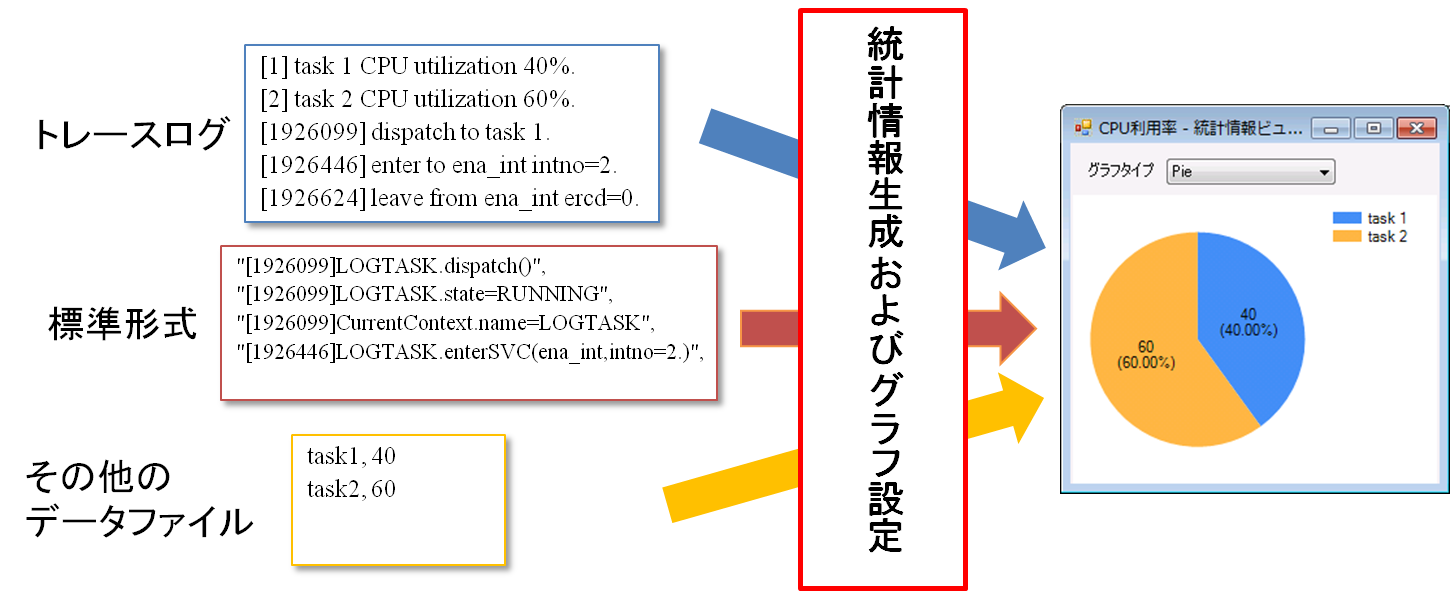
\includegraphics[scale=0.5]{statsabs.png}
\caption{���v���\���@�\�̊T�v�}}
\label{statsabs}
\end{center}
\end{figure}

\section{�݌v}\label{sec:sd_d}
���v�����O���t�Ƃ��ĕ\������ɂ́C���v���ƁC�O���t�̎�ނ�ڐ����Ȃǂ̃O���t
�̐ݒ肪�K�v�ł���D����āC���v���\���@�\�̏����Ƃ��āC���v�����擾�E������
��v���Z�X�ƃO���t�ݒ������v���Z�X���K�v�ƂȂ�D�����̃v���Z�X�𐧌䂷�邽��
�C���v���̐������@�ƃO���t�̐ݒ���w�肷��d�g�݂��C�ϊ��E�Ž������[���ɓ��l�ɁC
���v��񐶐����[���Ƃ��Č`�������Ē�`���邱�ƂŎ�������D

�{�߂ł́C���v���ƃO���t�Ɋւ���v������C�O���t�̐ݒ�C���v���̎擾�E�������@�������������ʂ��q�ׂ���C���v���ƃO���t�̐ݒ�̕ۑ����@�ɂ‚��Č����������ʂ��q�ׂ�D
\subsection{���v���̃O���t�\��} \label{sec:sd_d_gra}
���v���ɂ���ēK�؂ȃO���t��O���t�̐ݒ�͂��܂��܂ł���D���������āC�ǂ̂�
���ȃO���t�����p�ł��C�ǂ̂悤�ȃO���t�ݒ肪�ł���Ƃ悢�������[�U�ɑ΂��ăA��
�P�[�g���������{�����D�A���P�[�g�ɂ����͒������̂́CTLV���[�U�ł���NCES����
��1���Ɩ��É���w��w�@�̊w��1���̌v2���ł���D�u�ǂ̂悤�ȃO���t�łǂ̂悤�ȓ��v��
���\�����������v�Ƃ����₢�ɑ΂���񓚂��܂Ƃ߂����̂�\tabref{gtype}
�C�u�ǂ̂悤�ȃO���t�ݒ肪�s����Ƃ悢���v�Ƃ����₢�ɑ΂���񓚂��܂Ƃ߂�����
��\tabref{gset}�ł���D

\begin{table}[H]
\centering
\caption{��F�ǂ̂悤�ȃO���t�łǂ̂悤�ȓ��v����\����������}
\label{gtype}
\begin{tabular}{|l|p{4zw}|p{4zw}|p{4zw}|p{4zw}|p{4zw}|p{4zw}|}
\hline
���v��� &  �~ & �c�_ & ���_ & �܂�� & �q�X�g�O���� & �낤����
\\\hline\hline
�^�X�N��CPU���p�� &  �� &  &  &  &  & \\\hline
�������A�N�Z�X�� &  �� &  &  &  &  & \\\hline
�A�C�h������ &  �� &  &  &  &  & \\\hline
CPU�̏������Ԋ��� &  �� &  ��& �� &  &  & \\\hline
�^�X�N�̍��v���s���� &   &  ��& �� &  &  & \\\hline
�^�X�N�̎��s���ԕ��z &   &  &  &  & �� & \\\hline
�^�X�N�̐ؑ։� &   & �� &  & \shortstack[l]{��\\(���n��)} &  & \\\hline
�f�b�h���C���~�X�� &   & �� &  & \shortstack[l]{��\\(���n��)} &  & \\\hline
�^�X�N�̋N���� &   & �� &  & \shortstack[l]{��\\(���n��)} &  & \\\hline
\shortstack[l]{�^�X�N�N���v���L���[\\�C���O��} &   & �� &  & \shortstack[l]{��\\(���n��) }&  & \\\hline
�^�X�N�̉������� &   &  &  &  & �� & ��\\\hline
�����݋֎~���� &   &  &  &  & �� & ��\\\hline
\shortstack{���b�N�l�����Ԃ�\\�l���҂�����} &   &  &  &  & �� & ��\\\hline
\shortstack{�Z�}�t�H�l�����Ԃ�\\�l���҂�����} &   &  &  &  & �� & ��\\
\hline
\end{tabular}
\end{table}


\begin{table}[H]
\centering
\caption{��F�ǂ̂悤�ȃO���t�ݒ肪�s����Ƃ悢��}
\label{gset}
\begin{tabular}{|l|p{4zw}|p{4zw}|p{4zw}|p{4zw}|p{4zw}|p{4zw}|}
\hline
�O���t�ݒ� &    �~ & �c�_ & ���_ & �܂�� & �q�X�g�O���� & �낤����
\\\hline\hline
�^�C�g�� &  �� & �� & �� & �� & �� & ��\\\hline
X�l�̃��x�� &  �� & �� & �� & �� & �� & ��\\\hline
Y�l�̃��x�� &  �� & �� & �� & �� & �� & ��\\\hline
���̃^�C�g�� &   & �� & �� & �� & �� & ��\\\hline
�}�� &   & �� & �� & �� & �� & ��\\\hline
�O���b�h���̗L�� &   & �� & �� & �� & �� & ��\\\hline
�ڐ��� &   & �� & �� & �� & �� & ��\\\hline
\end{tabular}
\end{table}

�O���t�̎�ނł́C������\������~�O���t�C�l��r��\������_�O���t�C�l�ω���
�\������܂���O���t�C���U��\������q�X�g�O�����C�ŏ��E�ő�E���ς�\������
�O���t\footnote{�Y������O���t�͕�������̂ŁC\tabref{gtype}�ł͉��Ɂu�낤�����v�Ƃ��Ă���}���K�v�Ȃ��Ƃ��킩�����D���z
�}�����ɓ���Ă������C�Y�����铝�v���͍��񓾂��Ȃ������D

�O���t�̐ݒ�ł́C���₷��ۂɂ��炩���߈�ʓI�Ȑݒ荀�ڂ��Ă��āC�K�X�C�lj�
�E�폜���s���Ē������D�������Ȃ���C�lj����폜������Ă��Ȃ��������߁C��ʓI��
�ݒ荀�ڂ�����΁C���Ȃ��Ƃ������Ƃ��킩�����D����āC\tabref{gset}
�ɋ������O���t�̐ݒ��p�ӂ��邱�ƂɂȂ邪�C�����͎��̂悤�ɕ��ނł���D
�Ȃ��C�ݒ�̖��O�ƃO���t�ɂ����锽�f�ꏊ�ɂ‚��Ă�\figref{fig:graph}�Ɏ����D

\begin{figure}[ht]
\begin{center}
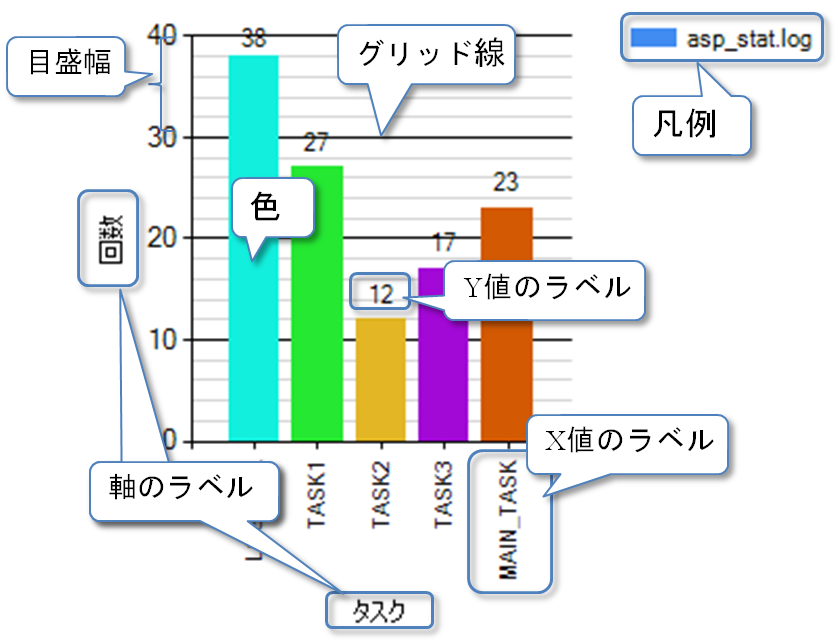
\includegraphics[scale=0.6]{graph.png}
\caption{�O���t�ݒ�̖��O�Ɣ��f�ꏊ}
\label{fig:graph}
\end{center}
\end{figure}

\begin{description}
\item[�f�[�^�|�C���g�Ɉˑ����Ȃ��ݒ�] \mbox{} \\
�^�C�g���C���̃^�C�g���C�}��C�O���b�h���̗L���C�ڐ���
\item[�f�[�^�|�C���g�Ɉˑ�����ݒ�] \mbox{} \\
X�l�̃��x���CY�l�̃��x���C�F
\end{description}

�����ŁC�f�[�^�|�C���g�Ƃ́C���v���̊e�f�[�^�̂��Ƃł���D����āC�g���[�X���O�Ȃǂ̓��v����
�\�[�X���قȂ�΁C�f�[�^�|�C���g���ω�����D��̓I�ɂ́C�Ⴆ�΃^�X�N�̋N����
�������߂ăO���t�ɕ\������Ƃ��CX���Ƀ^�X�N1�C�^�X�N2�C...�ƕ��ׂĕ\�����邽��
�̂��̂�X�l�̃��x���ł���C�v���b�g���ꂽ�e�f�[�^�|�C���g�t�߂ɂ��ꂼ�ꋁ�߂�
�񐔂̐�����\�����邽�߂̂��̂�Y�l�̃��x���ł���D

�f�[�^�|�C���g�Ɉˑ����Ȃ��ݒ�́CX�l��Y�l���O���t���ƂɈقȂ��Ă��Ă��C���v��
��̎�ނ������ł���΃O���t�ԂňقȂ邱�Ƃ͂Ȃ��D����āC�f�[�^�|�C
���g�Ɉˑ����Ȃ��ݒ�́C����̓��v�����O���t�\������ۂ̐ݒ�e���v���[�g�Ƃ�
�čė��p���邱�Ƃ��”\�ł���D������������邱�ƂŁC�ݒ�̏璷��h���C�������
�̓��v���Ɋւ��铝�v��񐶐����[�����L�q�����Ԃ��y���ł���D
\subsection{���v���̐����E�擾}\label{sec:dgen}
\subsubsection{���v���̃\�[�X�Ǝ擾�E�������@}\label{sec:dgenw}
���v�����擾�E��������v���Z�X�ł́C�܂��C���v���̃\�[�X���K�v�ł���D
�l������\�[�X�Ƃ��āC�g���[�X���O�Ƃ���ȊO�̌`���̃t�@�C���ł���D
����ȊO�̌`���̃t�@�C���Ƃ́C�V�X�e���̏o�́C�܂��́C����ȊO�̕��@�œ���ꂽ�t
�@�C���̂��Ƃł���D

���ɁC���v�����擾�E��������v���Z�X�ł́C�擾�E����������@���K�v�ł���D
�����ł����擾�Ƃ́C���炩�̌`�œ���ꂽ���v����TLV���ǂݎ�邱�Ƃ������C
�����Ƃ́C�\�[�X����͂�����C�\�[�X�ɂ���f�[�^�����Z���������肷�邱�Ƃœ��v���𓾂邱�Ƃ������D�\�[�X���g���[�X���O�̏ꍇ�C�g���[�X���O�ɂ����鎞�n�������͂��ē��v���𓾂邱�Ƃ��l������D�܂��C�V�X�e���������œ���ꂽ���v�����g���[�X���O�Ƃ��ďo�͂���ꍇ�C�����ǂݎ�邱�Ƃœ��邱�Ƃ��l������D
�\�[�X���g���[�X���O�ȊO�̌`���̃t�@�C���̏ꍇ���C�g���[�X���O�Ɠ��l�ɁC�t�@�C�����̃f�[�^����͂���C�t�@�C���ɋL�q����Ă��铝�v����ǂݎ��C�Ƃ��������Ƃœ��v���𓾂邱�Ƃ��l������D

����āC�擾�E���������̓I�ȕ��@��3��ލl�����D���������Ɏ����D

\begin{description}
\item[�������@1�F���K�\���ɂ��f�[�^�擾] \mbox{} \\
������̃}�b�`���O�Ȃ̂ŁC�g���[�X���O�₻��ȊO�̃t�@�C���ɂ��Ή��ł���D
�C���[�W��\figref{fig:seisei1}�Ɏ����D
\end{description}
\begin{figure}[h]
\begin{center}
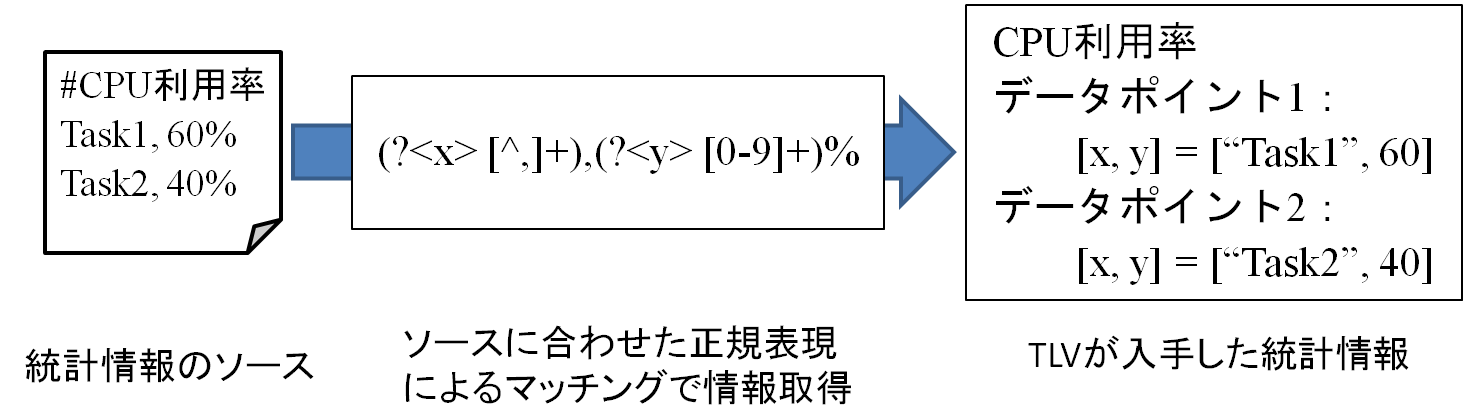
\includegraphics[scale=0.5]{seisei1.png}
\caption{�������@1�̃C���[�W}
\label{fig:seisei1}
\end{center}
\end{figure}
\begin{description}
\item[�������@2�F�O���v���Z�X�ɂ��擾�E����] \mbox{} \\
�X�N���v�g��A�v���P�[�V�����Ȃǂ��O���v���Z�X�Ƃ��ė��p���邱�ƂŁC���G�Ȍv�Z��
�K�v�ȓ��v����������D�܂��C���p����A�v���P�[�V���������Ή����Ă���΁C�l�X
�ȃt�@�C�����瓝�v��񂪓�����D
�C���[�W��\figref{fig:seisei2}�Ɏ����D
\end{description}
\begin{figure}[t]
\begin{center}
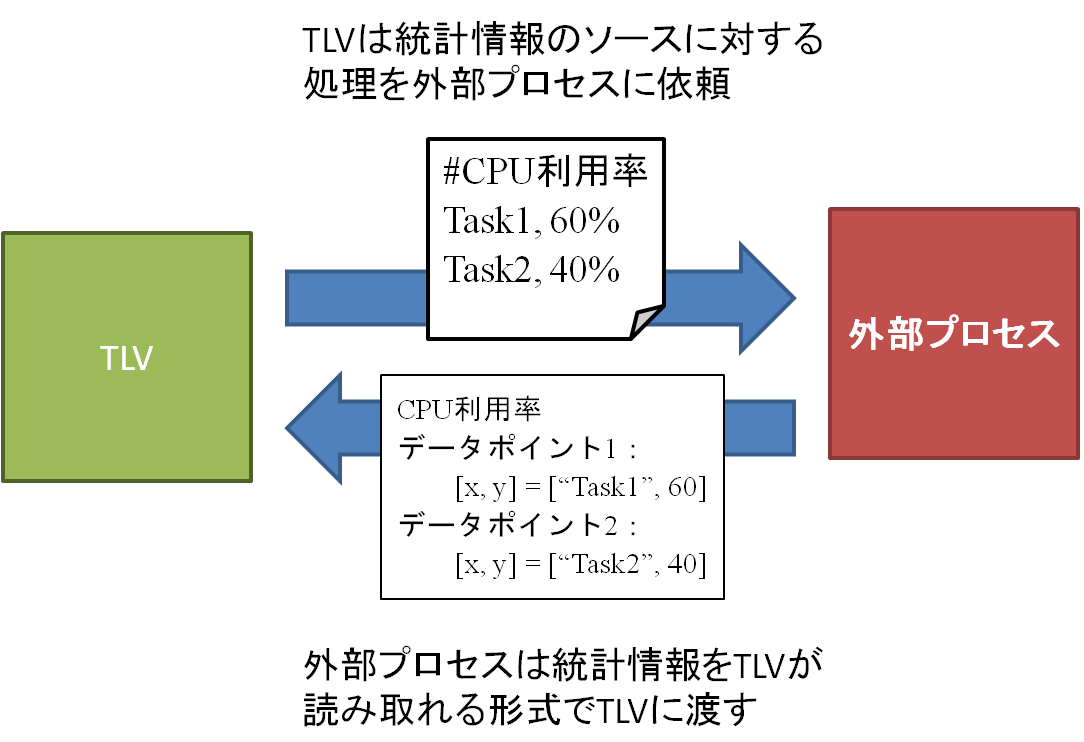
\includegraphics[scale=0.6]{seisei2.png}
\caption{�������@2�̃C���[�W}
\label{fig:seisei2}
\end{center}
\end{figure}
\begin{description}
\item[�������@3�FTLV�Ɏ��������ȒP�ȉ�͂��ł��郁�\�b�h�ɂ�鐶��] \mbox{} \\
�O���X�N���v�g�ł́C�J������R�X�g���ǂ����Ă��������Ă��܂��D���̂��߁C
TLV�ɕW���`���g���[�X���O���ȒP�ȉ�͂��ł��郁�\�b�h���������邱�ƂŁC
�O���X�N���v�g�𗘗p�����ɒP���ȓ��v��񂪐����”\�ɂȂ�D
�C���[�W��\figref{fig:seisei3}�Ɏ����D
\end{description}
\begin{figure}[h]
\begin{center}
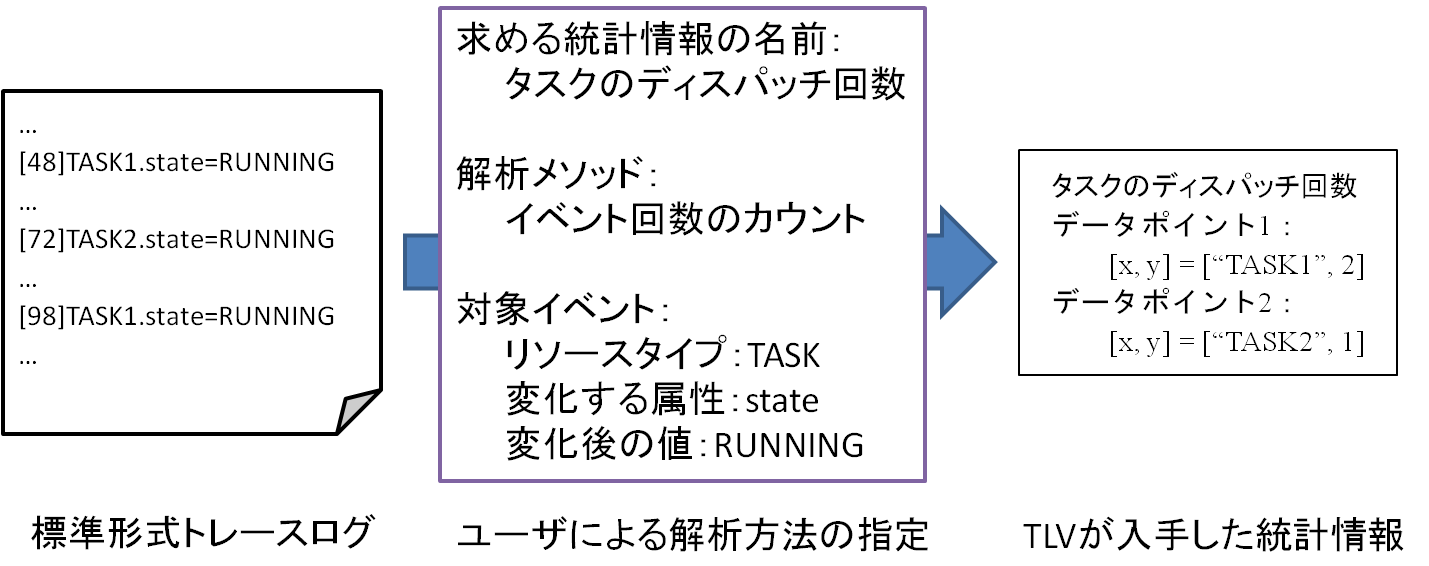
\includegraphics[scale=0.55]{seisei3.png}
\caption{�������@3�̃C���[�W}
\label{fig:seisei3}
\end{center}
\end{figure}

�������@3�Ɋւ��āC�O�q�̐��������ł͗������Â炢�̂ŁC�ڍׂ��q�ׂ�D

���̎�i�����[�U�ɒ񋟂���ɓ�����C�����‚��̊ȒP�ȉ�͂��ł��郁�\�b�h��TLV
�ɗp�ӂ���K�v������DTLV�ł́C���̃��\�b�h����̓��\�b�h�ƌĂԁD
\sref{sec:sd_d_gra}�Ɏ���\tabref{gtype}����C�g���[�X
���O�ɂ����铝�v���̎����ɂ‚��ĕ��͂������ʁC�K�v�ƂȂ郁�\�b�h�́C�C�x���g
�񐔂̃J�E���g�C�C�x���g�Ԋu�̑���C���肵���C�x���g�Ԋu�̃J�E���g��3�‚�
���邱�Ƃ��킩�����D�C�x���g�񐔂̃J�E���g�́C�^�X�N�̋N���񐔂Ȃǂ̃C�x���g�����������񐔂𐔂�����̂ł���D�C�x���g�Ԋu�̑���́C�n�_�ƂȂ�C�x���g����I�_�ƂȂ�C�x���g�܂ł̎��Ԃ𑪒肷����̂ł���D�����݋֎~���ԂȂǂ̎��ԂɊւ��铝�v���𓾂�ۂɕK�v�ƂȂ�D���肵���C�x���g�Ԋu�̃J�E���g�́C�q�X�g�O�����̐�����z�肵�Ă���C�C�x���g�Ԋu�̑�����s���ē���ꂽ���Ԃ����񂠂邩��������̂ł���D�Ⴆ�΁C�^�X�N�̎��s���ԕ��z�ȂǂŕK�v�ƂȂ�D

���v���̎����ɂ‚��ĕ��͂��Ă킩�������Ƃ͑��ɂ�����D
�e���\�b�h�́C�ΏۂƂȂ�C�x���g���w�肷��K�v�����邪�C���������v���ɂ���Ă�
�C���O�������K�v�ƂȂ�P�[�X������D�Ⴆ�΁C�^�X�N�̋N���́C�^�X�N���x�~��Ԃ���
���s�”\��ԂɂȂ�Ƃ��̂��Ƃ������D����āC�^�X�N�̋N���񐔂����߂�ۂ̑ΏۃC�x
���g�́C�^�X�N(TASK)�̏��(state)�����s�”\���(RUNNABLE)�ɑJ�ڂ���C�x���g
(�W���`���g���[�X���O�`���ŕ\�������``TASK.state=RUNNABLE'')�ƂȂ�D����
���C���̃C�x���g�́C�^�X�N�����s��Ԃł��鎞�ȂǕ����̏�Ԃɂ����Ĕ�������”\��
������D����āC�^�X�N�̋N���񐔂����߂�ɂ́C�ΏۃC�x���g�̑��Ɂu�^�X�N���x�~��
�Ԃł���v�Ƃ����O��������K�v�ɂȂ�D�����������P�[�X�͂ǂ̓��v���ɂ����肤��
�Ƃ����킯�ł͂Ȃ��̂ŁC�I�v�V�����ݒ�Ƃ��ėp�ӂ���D


\subsubsection{���v���𓾂�g���[�X���O��̎�����ԂƂ��̎w����@}
�g���[�X���O�₻�̑��̃t�@�C�����瓝�v�����擾����ꍇ�C��񂪐ÓI�ł���̂ŁC
�\�[�X���ς��Ȃ�����C���͕s�ςł���D

�������C���v���𐶐�����ꍇ�C�\�[�X���̃f�[�^�̎����ɂ���āC���l���ς���Ă���D�g���[�X���O�ɂ����鎞�n�������͂���ꍇ�C��͂��鎞����Ԃɂ���ĈقȂ�D

��͂��鎞����Ԃ��w�肷��^�C�~���O�Ƃ��āC�g���[�X���O�̉�͍�ƑO�Ɖ�͍�ƒ���2�ʂ肪�l������D

�܂��C�g���[�X���O�̉�͍�ƑO�Ƃ́CTLV�Ƀg���[�X���O�Ȃǂ̓��͂�^����O�̂���
�ł���D���̏󋵂ŋ�Ԏw��”\�ł��邱�Ƃ́C���Ȃ킿�C�w�肷���Ԃ����łɌ��܂�
�Ă����Ԃł���D��̓I�ɂ́C��ԂƂ��ăg���[�X���O�S�̂��w�肵�����ꍇ�Ȃǂł�
��D���̂悤�ȏꍇ�C���v���𓾂悤�Ƃ��邽�тɋ�Ԏw����s���͔̂������
����D����āC�O���t�@�C���ŋ�Ԃ��w�肵�Ă����CTLV�ɕϊ��E�Ž��������Ɠ����^�C
�~���O�œ��v�����擾�E�����ł���悤�ɂ��邱�ƂŁC����������D

���ɁC�g���[�X���O�̉�͍�ƒ��Ƃ́CTLV�Ńg���[�X���O���Ž������Ă����Ԃł���
�D�g���[�X���O�̉�͍�ƒ��ɂ́C��͂�e�Ղɂ��邽�߂ɁC����ꕔ��Ԃ݂̂̓��v��
�񂪕K�v�ɂȂ邱�Ƃ�����D����āC�Ž��������Ԃ���͂��ē��v���𓾂���悤
�ɂ���D�܂��C���̃P�[�X�ł́C�Ž������ꂽ�g���[�X���O�������Ă��邽�߁CGUI��p
���ăO���t�B�J���Ɏw��ł���悤�ɂ��邱�ƂŁC���p���₷������D

�g���[�X���O�ȊO�̃t�@�C���ł��C�\�[�X���̃f�[�^�̎����ɂ���Đ��l���ς���Ă�
�邪�C�\�[�X���̃f�[�^��`������ӂɒ�܂�Ȃ����߁C�g���[�X���O�̉�͂Ɠ��l�̋@
�\��TLV�Ŏ������Ȃ����Ƃɂ���D
\subsection{���v���ƃO���t�ݒ�̕ۑ����@}
�擾�E�����������v���ƃO���t�ݒ�̕ۑ����@�ɂ‚���3�‚̌��������Č��������D
\figref{fig:statsfile}�Ɏ����D�ȉ��ɂ��ꂼ��̗��_�E���_���q�ׁC
�����������e�������D

\begin{figure}[ht]
\begin{center}
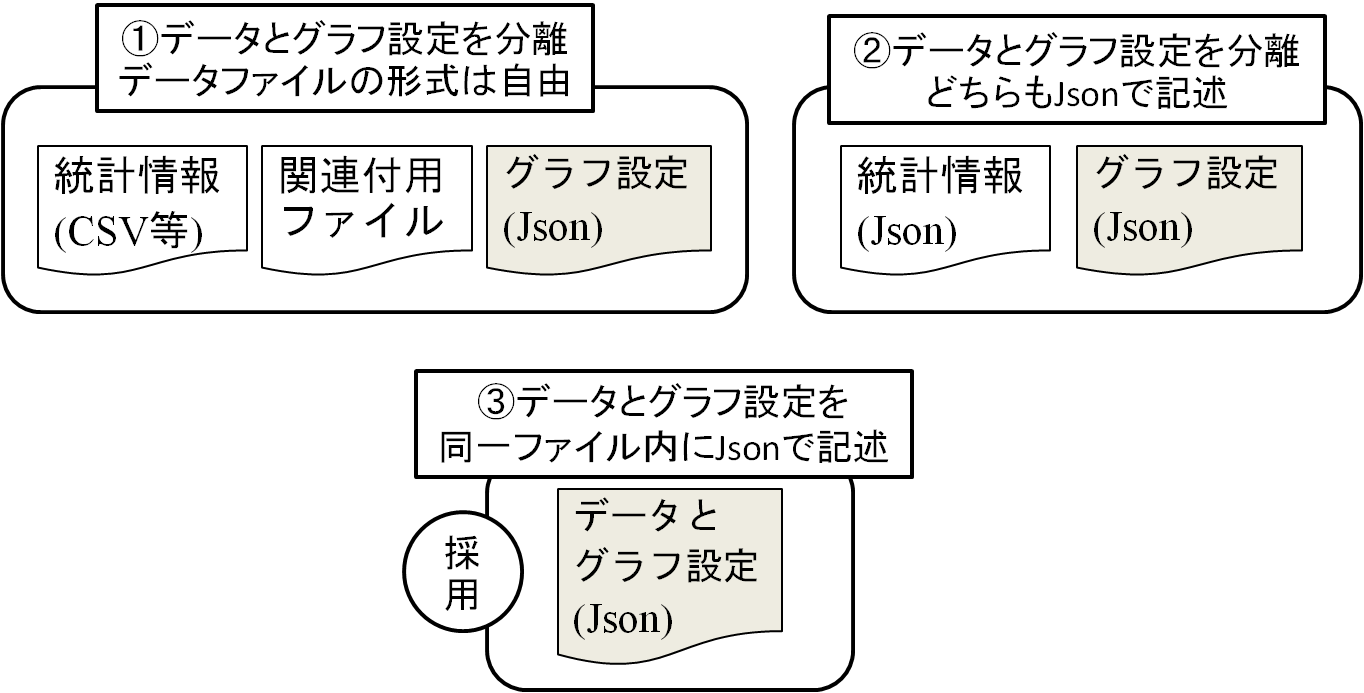
\includegraphics[scale=0.6]{statsfile.png}
\caption{���v���ƃO���t�ݒ�̕ۑ����@�̌��}
\label{fig:statsfile}
\end{center}
\end{figure}

���1�́C�f�[�^�|�C���g�Ɉˑ����Ȃ��O���t�ݒ�Ɠ��v�������ꂼ��ʂ̃t�@�C���ŕۑ�������@�ł���D�֘A�t�p�t�@�C���́C���v���ƃO���t�ݒ�̂��ꂼ���ۑ�����t�@�C���̃p�X�܂��͎��ʎq���L�q���C���v����ۑ�����t�@�C������f�[�^�����o���Ƃ��Ɏg�p���鐳�K�\�����L�q����D�f�[�^�|�C���g�Ɉˑ�����O���t�ݒ�́C���v����ۑ�����t�@�C���Ƀf�[�^�|�C���g�Ɗ֘A�t���ċL�q����D���̕��@�ɂ‚��Ă̗��_�ƌ��_�����Ɏ����D
\paragraph{���1�̗��_}
\begin{itemize}
\item  ���v����ۑ�����t�@�C���̃t�@�C���`����l�X�ȕ��@�ŕۑ��ł���悤�ɂ��邱�ƂŁCTLV�ȊO�̃A�v���P�[�V�����ł����v���𗘗p�ł���悤�ɂȂ�D

\item �f�[�^�|�C���g�Ɉˑ����Ȃ��O���t�ݒ���ė��p�ł���悤�ɂȂ�C�O���t�ݒ��ۑ�����t�@�C����1�•ύX���邾���ŁC���̕ύX���֌W���铝�v��񂷂ׂĂɔ��f�����D
\end{itemize}

\paragraph{���1�̌��_}
\begin{itemize}
\item �t�@�C���𕪎U�����邱�ƂŁC���v��񂪂ǂ̂悤�ȃO���t�ݒ�ŕ\������邩���c�����Â炢�D

\item �t�@�C���ړ��Ɏア�D�֘A�t�p�t�@�C�����X�V���Ȃ���΂Ȃ�Ȃ��D

\item �Ǘ�����t�@�C�������2���3��葽���̂ŕێ琫���ቺ����D

\item ���v����ۑ�����t�@�C���𑼂̃A�v���P�[�V�����Ŏg�p����ꍇ�C���v���Ƃ͖��֌W�̏��ł���f�[�^�|�C���g�Ɉˑ�����O���t�ݒ肪�����̏�Q�ƂȂ�D

\item TLV�̎g�p�‹��ɂ��C�O���t�ݒ��ۑ�����t�@�C���̓��e���قȂ�ꍇ������̂ŁC���v����ۑ�����t�@�C���������قȂ�‹��ֈڂ��ƁC�ړ��O�̊‹��Ɠ����O���t�ݒ�ŃO���t�D

\item ���v���̎�ނɂ���ẮC�ڐ����Ȃǂ̃O���t�ݒ�����O���Ƃɐݒ肵�����P�[�X������̂ŁC���̑Ή�������D

\item ���K�\���͉“ǐ����Ⴍ�C����`���̃t�@�C���ɂ͑Ή����Â炢�D
\end{itemize}


���2�́C���1���l�Ƀt�@�C���������s�����C�ǂ����JSON�ŋL�q������@�ł���D���1�ł̊֘A�t�p�t�@�C���̑���ɁC���v����ۑ�����t�@�C���ɃO���t�ݒ��ۑ�����t�@�C���̃p�X�܂��͎��ʎq���w�肷��D���̕��@�ɂ‚��Ă̗��_�ƌ��_�����Ɏ����D
\paragraph{���2�̗��_}
\begin{itemize}
\item �f�[�^�|�C���g�Ɉˑ����Ȃ��O���t�ݒ���ė��p�ł���悤�ɂȂ�C�O���t�ݒ��ۑ�����t�@�C����1�•ύX���邾���ŁC���̕ύX���֌W���铝�v��񂷂ׂĂɔ��f�����D
\item ���1�̌��_�ł������ێ琫�̌��O�ƃf�[�^�|�C���g�Ɉˑ�����O���t�ݒ�̖�肪�ɘa�����D
\end{itemize}

\paragraph{���2�̌��_}
\begin{itemize}
\item �t�@�C���𕪎U�����邱�ƂŁC���v��񂪂ǂ̂悤�ȃO���t�ݒ�ŕ\������邩���c�����Â炢�D

\item ���v����ۑ�����t�@�C���𑼂̃A�v���P�[�V�����ŗ��p�ł��Ȃ��D

\item TLV�̎g�p�‹��ɂ��C�O���t�ݒ��ۑ�����t�@�C���̓��e���قȂ�ꍇ�����邽�߁C�قȂ�‹��ł̃O���t�ݒ肪�ۏႳ��Ȃ��D

\item ���v���̎�ނɂ���ẮC�ڐ����Ȃǂ̃O���t�ݒ�����O���Ƃɐݒ肵�����P�[�X������̂ŁC���̑Ή�������D
\end{itemize}

���3�́C���v�����O���t�ݒ��1�‚̃t�@�C���ɕۑ�������@�ł���D���̕��@�ɂ‚��Ă̗��_�ƌ��_�����Ɏ����D

\paragraph{���3�̗��_}
\begin{itemize}
\item ���v��񂪂ǂ̂悤�ɃO���t�\������邩�c�����₷���D

\item 1�‚̃t�@�C���݂̂Ŋ�������̂ŁC�t�@�C���p�X�Ȃǂ̐��������C�ɂ��Ȃ��ėǂ��D

\item ���v��񖈂ɃO���t�ݒ肪�ł���D

\item �������y�ł���D
\end{itemize}

\paragraph{���3�̌��_}
\begin{itemize}
\item ���v����ۑ�����t�@�C���𑼂̃A�v���P�[�V�����ŗ��p�ł��Ȃ��D

\item �����O���t�ݒ肪�����̃t�@�C���ɏo�����ď璷����D�C������ꍇ�Ɏ��Ԃ�������D
\end{itemize}

���1�́C���̃A�v���P�[�V�����̎g�p���Œ���ɂ���ړI���炷��ƁC���_�ɔ�ח��_���ア�̂ŁC�c���2�‚ɍi����D���2�ƌ��3�ł́C�����̊ϓ_���炷��ƁC�ǂ�������ׂ�JSON�ŋL�q����̂ŁC���2������3�ւ̕ύX�C�܂��́C���̋t�̕ύX���e�Ղɍs����ƍl������D����āC�������Ԃ��l�����āC�܂��͗e�ՂɎ����ł��C���_�����Ȃ����3���̗p�����D���̓��v���ƃO���t�ݒ���܂񂾃t�@�C���̂��Ƃ𓝌v���t�@�C���ƌĂԂ��Ƃɂ���D



\section{����}\label{sec:sd_impl}
�{�߂ł́C\sref{sec:sd_d}�̐݌v�Ɋ�Â��������ɂ‚��ďq�ׂ�D

\subsection{���v���\���@�\�̎�ȃv���Z�X}

\begin{figure}[ht]
\begin{center}
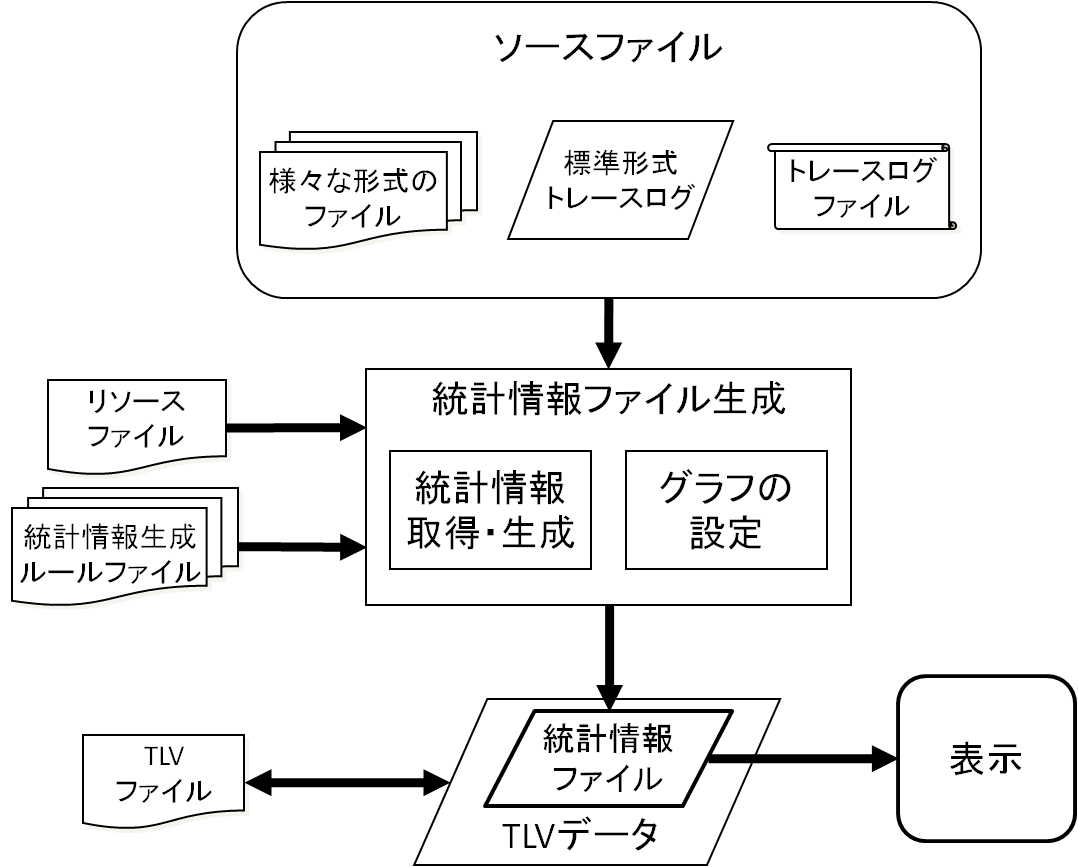
\includegraphics[scale=0.6]{stats_process.png}
\caption{���v���\���@�\�̏����v���Z�X}
\label{fig:sdproc}
\end{center}
\end{figure}

���v���\���@�\�́C���v�����O���t�\�����邽�߂̃t�@�C���𐶐�����v���Z�X
��6��ނ̃t�@�C���ɂ���Ď��������D\figref{fig:sdproc}�ɓ��v���\���@�\��
��ȃv���Z�X�������D

���v���t�@�C���𐶐�����v���Z�X�ł́C���v��񐶐����[���t�@�C���ɋL�q���ꂽ���v��񐶐����[���ɏ]���C�w�肵���\�[�X���瓝�v�����擾�E��������D�����āC����
�ꂽ���v���ƁC���v��񐶐����[���ɏ]�����O���t�̐ݒ��1�‚̃t�@�C���ɏ�������
�C�Ƃ������������s���D���̃v���Z�X�ł́C���v���̃\�[�X�ƂȂ�3�‚̃t�@�C��
(�ϊ����̃g���[�X���O�C�W���`���g���[�X���O�C�g���[�X���O�ȊO�̃t�@�C��)
�̂����̂ǂꂩ1�‚ƁC���v��񐶐����[���t�@�C���C���v���
�̐�����O���t�̐ݒ�Ɋ֌W���郊�\�[�X�t�@�C�����ǂݍ��܂��D

\figref{fig:sdproc}�ł́C���v�����擾�E��������v���Z�X�ƃO���t�ݒ���s���v��
�Z�X���C���v���t�@�C���𐶐�����v���Z�X�̃T�u�v���Z�X�Ƃ��ĕ\�����Ă��邪�C
�����2�‚̃v���Z�X�����ꂼ��Ɨ����ē��삷��Ƃ͌���Ȃ����Ƃ������Ă���D
���Ƃ��΁C���v���𐶐����‚C�e�f�[�^��\���F���•ʂɐݒ肷��Ƃ������P�[
�X���Y������D

�����������v���t�@�C���́C���v���r���[�A�ƌĂ΂�铝�v�����O���t�\����
�邽�߂̃E�B���h�E�ŗ��p�����D�܂��CTLV�f�[�^���Ɋi�[���邱�ƂŁCTLV�t�@�C
���Ƃ��ĊO���t�@�C���ɕۑ��ł��C�����g���[�X���O�������ۂɍēx�C���v���t�@
�C���𐶐����Ȃ��Ă��悭�Ȃ�D


\subsection{���v���\���@�\����������TLV�̏����v���Z�X}
�K�v�ȓ��v���𓾂邽�߂ɂ́C���[�U��TLV�ɓ��v��񐶐����[������͂���K�v������D�����ł܂��l��������@�́C�g���[�X���O�ƃ��\�[�X�t�@�C������͂�����@�Ɠ��l�ɁCGUI�Ŏw�肷����@�ł���D�������Ȃ���C�^�[�Q�b�g�V�X�e�����f�o�b�O����ہC�g���[�X���O�����x����蒼���CTLV�ʼn��x���ϊ��E�Ž������������邱�ƂɂȂ�̂ŁC���̂��тɓ��v��񐶐����[������͂��邱�ƂɂȂ�D���̂��߁C���̕��@�����ł́C���͍�Ƃ�������ɂȂ�D����āC�܂��C�]����TLV�̏����v���Z�X�œ��v���t�@�C�������v���Z�X�����s������@����������D


\begin{figure}[ht]
\begin{center}
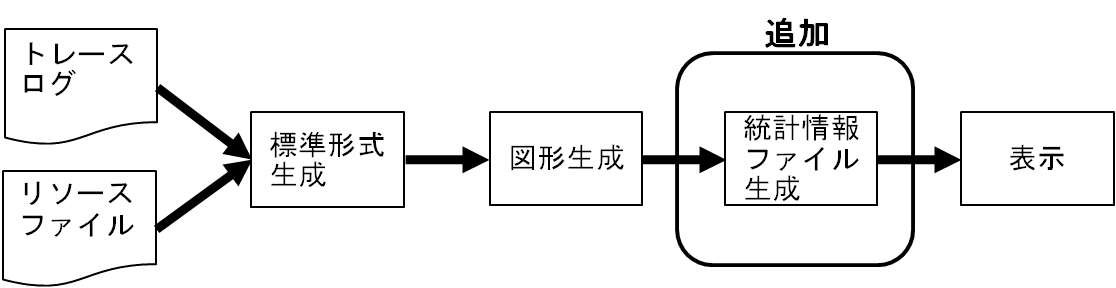
\includegraphics[scale=0.6]{tlv_addstats.png}
\caption{���v���\���@�\����������TLV�̏����v���Z�X}
\label{fig:newproc}
\end{center}
\end{figure}

�]����TLV�̏����v���Z�X�́C\sref{sec:tlv_d}�Ŏ������ʂ�C�g���[�X���O�ƃ��\�[�X�t�@�C����ǂݍ��݁C�g���[�X���O��W���`���g���[�X���O�֕ϊ����C�}�`�f�[�^��������v���Z�X�ƂȂ��Ă���D�ϊ��Ɛ}�`�f�[�^�����Ɏg�p����ϊ����[���ƉŽ������[���́C���\�[�X�t�@�C���Œ�`����Ă���D

���v���\���@�\����������TLV�̏����v���Z�X��\figref{fig:newproc}�Ɏ����D
�]���̃v���Z�X�ɂ���}�`�f�[�^�����v���Z�X�̌�ɁC���v���\���@�\�̏����v���Z�X�ł���
���v���t�@�C�������v���Z�X��lj�����`�ƂȂ�D���͂��铝�v��񐶐����[�������\�[�X�t�@�C���Œ�`���邱�ƂŁC���[�U�����ړ��͂���t�@�C�����𑝂₳���ɍςށD�܂��C�}\ref{resChangeSample}��{\tt "StatisticsGenerationRules"}�̂悤�ɁC���̃��[���Ɠ����w����@�ɂ��邱�ƂŁC���v���\���@�\�ɑ΂���w�K�R�X�g���y��������ʂ�����D

\begin{figure}[h]
\begin{lstlisting}
{
	"TimeScale" :"us",
	"TimeRadix" :10,
	"ConvertRules"   :["asp"],
	"VisualizeRules" :["toppers","asp"],
	"ResourceHeaders":["asp"],

	"StatisticsGenerationRules":["task_dispatch_count"],

	"Resources": {...}
}
\end{lstlisting}
\caption{���v���\���@�\�𗘗p���郊�\�[�X�t�@�C���̗�}
\label{resChangeSample}
\end{figure}


\subsection{���v���t�@�C��}
���v���t�@�C���Ƃ́C�O���t�̐ݒ�Ɠ��v��񂪌`���I�ɋL�q���ꂽ�t�@�C���̂��Ƃ�
����DTLV�ł́C���v���t�@�C�������v���Z�X�Ő�������C���v���r���[�A�ɃO���t
��\������Ƃ��Ɏg�p����D�܂��C���[�U�́CTLV�t�@�C����ʂ��ĊO���o�͂��邱�Ƃɂ��C���v���𐔒l�f�[�^�Ƃ��ē��邱�Ƃ��ł���D

���v���t�@�C���ɂ́C1�‚̓��v���Ɋւ��铝�v���t�@�C�����L�q�����D���v���t�@�C���̗��}\ref{statsfileformat}�Ɏ����D

\begin{figure}[h]
\begin{lstlisting}
{
  "task_dispatch_count": {
    "Setting":{
      "Title":"�^�X�N�̃f�B�X�p�b�`��",
      "AxisXTitle":"�^�X�N",
      "AxisYTitle":"��",
      "DefaultType":"Column",
      "MajorTickMarkInterval":10.0,
      "MinorTickMarkInterval":5.0,
      "MajorGridVisible":true,
      "MinorGridVisible":true
    },
    "Series": {
      "Points": [
        {
          "XLabel": "task 1",
          "XValue": 0,
          "YValue": 40
        },
        {
          "XLabel": "task 2",
          "XValue": 0,
          "YValue": 60
        }
      ]
    }
  }
}
\end{lstlisting}
\caption{���v���t�@�C���̗�}
\label{statsfileformat}
\end{figure}

\clearpage
\begin{description}
\item[\texttt{Setting}] \mbox{}
    \vspace{-0.25zw}
    \begin{description}
    \setlength{\itemsep}{-1.5mm}
    \item[����] �O���t�ݒ�̒�`
    \item[�l] �I�u�W�F�N�g�D�����o�̐����͈ȉ��̒ʂ�ł���D
    
            \begin{description}
            {\nopagebreak
            \item[\texttt{Title}] \mbox{}
            \vspace{-0.25zw}
                \begin{description}
                \setlength{\itemsep}{-1.5mm}
                \item[����] �O���t�̃^�C�g���D���GUI�\���ɗp������D
                \item[�l] ������
                \item[�ȗ���] ���v��񐶐����[�������K�p�����D
                \end{description}
            }{\nopagebreak
            \item[\texttt{AxisXTitle}] \mbox{}
            \vspace{-0.25zw}
                \begin{description}
                \setlength{\itemsep}{-1.5mm}
                \item[����] X���̃^�C�g���D
                \item[�l] ������
                \item[�ȗ���] �ݒ肳��Ȃ��D
                \end{description}
            }{\nopagebreak
            \item[\texttt{AxisYTitle}] \mbox{}
            \vspace{-0.25zw}
                \begin{description}
                \setlength{\itemsep}{-1.5mm}
                \item[����] Y���̃^�C�g���D
                \item[�l] ������
                \item[�ȗ���] �ݒ肳��Ȃ��D
                \end{description}
            }{\nopagebreak
            \item[\texttt{DefaultType}] \mbox{}
            \vspace{-0.25zw}
                \begin{description}
                \setlength{\itemsep}{-1.5mm}
                \item[����] �ŏ��ɕ\������O���t�̎�ށD
                \item[�l] ������(���݁C\verb|"Pie"|�F�~�C\verb|"Column"|�F�c�_�C\verb|"Bar"|�F���_�C\verb|"Line"|�F�܂���C\verb|"Histogram"|�F�q�X�g�O�����̂����ꂩ)
                \item[�ȗ���] \verb|"Pie"|
                \end{description}
            }{\nopagebreak
            \item[\texttt{MajorTickMarkInterval}] \mbox{}
            \vspace{-0.25zw}
                \begin{description}
                \setlength{\itemsep}{-1.5mm}
                \item[����] ��ڐ��̊Ԋu�D
                \item[�l] ���l
                \item[�ȗ���] �f�[�^�ɍ��킹�Ď����ݒ�D
                \end{description}
            }{\nopagebreak
            \item[\texttt{MinorTickMarkInterval}] \mbox{}
            \vspace{-0.25zw}
                \begin{description}
                \setlength{\itemsep}{-1.5mm}
                \item[����] �⏕�ڐ��̊Ԋu�D
                \item[�l] ���l
                \item[�ȗ���] �f�[�^�ɍ��킹�Ď����ݒ�D
                \end{description}
            }{\nopagebreak
            \item[\texttt{MajorGridVisible}] \mbox{}
            \vspace{-0.25zw}
                \begin{description}
                \setlength{\itemsep}{-1.5mm}
                \item[����] ��ڐ��̃O���b�h����\�����邩�ǂ����D������\verb|true|���w�肳�ꂽ�ꍇ�C�O���b�h�����\�������D
                \item[�l] �^�U�l
                \item[�ȗ���] \verb|false|
                \end{description}
            }
\clearpage
            {\nopagebreak
            \item[\texttt{MinorGridVisible}] \mbox{}
            \vspace{-0.25zw}
                \begin{description}
                \setlength{\itemsep}{-1.5mm}
                \item[����] �⏕�ڐ��̃O���b�h����\�����邩�ǂ����D������\verb|true|���w�肳�ꂽ�ꍇ�C�O���b�h�����\�������D
                \item[�l] �^�U�l
                \item[�ȗ���] \verb|false|
                \end{description}
            }
            \end{description}
    \end{description}
\item[\texttt{Series}] \mbox{}
    \vspace{-0.25zw}
    \begin{description}
    \setlength{\itemsep}{-1.5mm}
    \item[����] �n��D
    \item[�l] �I�u�W�F�N�g�D�B��̃����o�ł���\verb|Point|�͒l�Ƃ��ăI�u�W�F�N�g�̔z����Ƃ�D�z��Ɋi�[�����I�u�W�F�N�g�̓f�[�^�|�C���g��\���D�f�[�^�|�C���g��\���I�u�W�F�N�g�̃����o�̐����͈ȉ��̒ʂ�ł���D
    
            \begin{description}
            \setlength{\itemsep}{-1.5mm}
            {\nopagebreak
            \item[\texttt{XLabel}] \mbox{}
            \vspace{-0.25zw}
                \begin{description}
                \setlength{\itemsep}{-1.5mm}
                \item[����] X���ɕ��ׂ�f�[�^�|�C���g�̃��x���D
                \item[�l] ������
                \item[�ȗ���] �ݒ肳��Ȃ��D
                \end{description}
            }{\nopagebreak
            \item[\texttt{YLabel}] \mbox{}
            \vspace{-0.25zw}
                \begin{description}
                \setlength{\itemsep}{-1.5mm}
                \item[����] �f�[�^�|�C���g��ɕ\�����郉�x���D�~�O���t�ƃq�X�g�O�����ŕ\������Ƃ��͔��f����Ȃ��D
                \item[�l] ������(���̃}�N�����g�p�”\�D\verb|"#VALX"|�FX�l�C\verb|"#VALY"|�FY�l�C\verb|"#PERCENT"|�F�n��S�̂ɑ΂���Y�l�̊����C\verb|"#TOTAL"|�F�n��̑S�Ă�Y�l�̍��v)
                \item[�ȗ���] �O���t�ɍ��킹�Ď����I�ɐݒ肳���D
                \end{description}
            }{\nopagebreak
            \item[\texttt{XValue}] \mbox{}
            \vspace{-0.25zw}
                \begin{description}
                \setlength{\itemsep}{-1.5mm}
                \item[����] X�l�D
                \item[�l] ���l
                \item[�ȗ���] 0
                \end{description}
            }{\nopagebreak
            \item[\texttt{YValue}] \mbox{}
            \vspace{-0.25zw}
                \begin{description}
                \setlength{\itemsep}{-1.5mm}
                \item[����] Y�l�D
                \item[�l] ���l
                \item[�ȗ���] 0
                \end{description}
            }{\nopagebreak
            \item[\texttt{Color}] \mbox{}
            \vspace{-0.25zw}
                \begin{description}
                \setlength{\itemsep}{-1.5mm}
                \item[����] �O���t�Ƀv���b�g�����f�[�^�|�C���g�̐F�D
                \item[�l] ������(\verb|"#AARRGGBB"|�Ƃ����t�H�[�}�b�g�ɏ]���DA�F�A���t�@�l�CR�F�ԁCG�F�΁CB�F�‚Ƃ��C16�i���ŕ\������)
                \item[�ȗ���] �O���t���C�u�����̏����l�ɏ]���D
                \end{description}
            }
            \end{description}
    \end{description}
\end{description}
    
\subsection{���v���̎擾�E����}
���v���̎擾�E�����́C\sref{sec:dgenw}�ɂāC3�ʂ�̎�i���l�����D������
�������@���������C���v���̃\�[�X�ƂȂ�t�@�C����p�r�ɍ��킹�đI���ł���悤�����D�����̎������@��p���ē��v�����擾�E�������ē��v���t�@�C���𐶐������i�𐶐����[�h�ƌĂԁD�������[�h�́C����4��ނł���D
\begin{itemize}
\item �f�[�^�ǂݎ�胂�[�h(\sref{sec:dgenw}�ɂ�����������@1)
\item �X�N���v�g�g�����[�h(\sref{sec:dgenw}�ɂ�����������@2)
\item ��{��̓��[�h(\sref{sec:dgenw}�ɂ�����������@3)
\item ���v���t�@�C�����̓��[�h
\end{itemize}
�����̐������[�h�́C���v��񐶐����[���Őݒ肷��D

�������[�h�ł́C��{�I�ɓ��v���̎擾�E�����ƃf�[�^�|�C���g�Ɉˑ�����O���t�ݒ�݂̂��s�����C�X�N���v�g�g�����[�h�Ɠ��v���t�@�C�����̓��[�h�Ɋւ��Ă͂��̌���ł͂Ȃ��D�ڂ����́C���ꂼ��̃��[�h�����ŏq�ׂ�D


\subsubsection{�f�[�^�ǂݎ�胂�[�h}\label{sec:datin}
\begin{description}
\item[�ΏۂƂȂ�\�[�X�t�@�C��] \mbox{} \\�g���[�X���O�C�W���`���g���[�X���O�C���̑��̃t�@�C��
\end{description}
�f�[�^�ǂݎ�胂�[�h�Ƃ́C\sref{sec:dgenw}�ɂ�����������@1����������
�������[�h�ł���D���K�\���̃}�b�`���O�̍ۂɖ��O�t���O���[�v���\���̂�p���ĕ���
��������L���v�`�����CX�l��Y�l���擾����D�K�v�ɉ����āC�O���t��̊e�f�[�^�̐F��
�ݒ�ł���悤�ɂ��邱�ƂŁC�O���t�����₷���ł���悤�ɂ����D

���K�\���́C������`�ł���悤�ɂ����D�������邱�ƂŁC�������v���ɑ΂��ĈقȂ�\
��������Ă���P�[�X�ɑΉ��ł��C�܂��C�}�b�`���O���鐳�K�\���ɂ���ĈقȂ�F���
��ł���悤�ɂȂ�D�F�̐ݒ�Ɋւ����̓I�ȃP�[�X�́CX�������\�[�X�ƂȂ�Ƃ���
���\�[�X�ʂɐF��ݒ肷��P�[�X�CY�l�����鐔�l�ȏ�ƂȂ�f�[�^�݂̂��ق��̐F�ɐ�
�肷��P�[�X�Ȃǂ�����D


\subsubsection{�X�N���v�g�g�����[�h}
\begin{description}
\item[�ΏۂƂȂ�\�[�X�t�@�C��] \mbox{} \\�g���[�X���O�C�W���`���g���[�X���O�C���̑��̃t�@�C��
\end{description}
�X�N���v�g�g�����[�h�Ƃ́C\sref{sec:dgenw}�ɂ�����������@2���������鐶�����[�h�ł���D

���̐������[�h�̖��O�́C�ϊ����[���C�Ž������[���ɂ�����X�N���v�g�g���@�\�ɗR��
����D���O�ȊO�ɂ��C���o�͂ɑ����̍��ق�������x�ŁC����ȊO�͂قڂ����ɍ��킹
�������ɂ����D����́C���łɂ���@�\�ɍ��킹�邱�ƂŁC�g�p���@�̏K����e�Ղɂ���
���߂ł���D�܂��C�J���̊ϓ_�ł͕ێ琫�����߂邱�Ƃɂ‚Ȃ���D

��ɃX�N���v�g�𗘗p���邱�Ƃ�z�肵�Ă���̂ŁC�����ł͂���ɏ]���ď����v���Z�X
���������D�܂��CTLV�͓��v��񐶐����[���Ŏw�肳�ꂽ�X�N���v�g�����n�ƃX�N���v�g�{
�̂��O���v���Z�X�Ƃ��ċN������D���ɁC�N�������O���v���Z�X�̕W�����͂ɑ΂��C���\
�[�X�t�@�C���ƑΏۂƂȂ�\�[�X�t�@�C�����o�͂���D�O���v���Z�X�́C�W�����͂ɏ���
���܂ꂽ2�‚̃t�@�C����ǂݍ���ŏ������s���C�W���o�͂ɓ��v���t�@�C����������
�ށD�����āCTLV���O���v���Z�X�̕W���o�͂ɏ������܂ꂽ���v���t�@�C����ǂݍ���
�C�������[�h�̏������I����D

�O���v���Z�X�Ƃ��ċN������A�v���P�[�V�����Ɋւ��ẮC�W�����͂Ń��\�[�X�t�@�C��
�ƑΏۂƂȂ�\�[�X�t�@�C����ǂݍ��݁C�W���o�͂ɓ��v���t�@�C�����������ށC�Ƃ�
����߂�ꂽ���o�͎d�l�𖞂����Ă���΂悢�D

�ȏ�̂悤�ɁC���̐������[�h�ł͊O���v���Z�X����擾�E�����������v���𓝌v���
�t�@�C���Ƃ����`�Ŏ󂯎��D����́C�擾�E�����������v���ƃf�[�^�|�C���g�Ɉˑ�
����O���t�ݒ�����ѕt�����f�[�^���O���v���Z�X����󂯎��₷������ق��ɁC�f�[
�^�|�C���g�Ɉˑ����Ȃ��O���t�ݒ���O���v���Z�X���Őݒ肵�����P�[�X�ɑΉ����邽��
�ł���D�Ⴆ�΁C�ڐ��Ԋu��������������P�[�X��C\sref{sec:datin}��
�������F�Ɋւ���P�[�X�ł���D



\subsubsection{��{��̓��[�h}
\begin{description}
\item[�ΏۂƂȂ�\�[�X�t�@�C��] \mbox{} \\�W���`���g���[�X���O
\end{description}
��{��̓��[�h�Ƃ́C\sref{sec:dgenw}�ɂ�����������@3���������鐶�����[�h�ł���D���̐������[�h�́C���[�U����̓��\�b�h�Ƃ���ɕK�v�ȏ���^���邱�ƂŁC���v���𐶐�����D

���̐������[�h���ΏۂƂ���\�[�X�t�@�C���͕W���`���g���[�X���O�݂̂ł���D����́CTLV���l�X�ȃg���[�X���O��������悤�ɁC�g���[�X���O��W���`���g���[�X���O�Ƃ������Ԍ`���ɂ���̂ŁC����𗘗p���邱�ƂŔėp�I�ȉ�̓��\�b�h��P���Ȍ`�Œ񋟂ł��邩��ł���D�l�X�Ȍ`���ɑΉ��������̂ɂ��Ă��܂��ƁC���K�\���ɂ��}�b�`���O���K�v�ɂȂ�D���̌��ʁC�������[�h�̎w�肪���G�Ȍ`�ƂȂ邤���C���v��񐶐����[���t�@�C���ɋL�q����ۂɉ“ǐ����Ⴍ�Ȃ�C���̐������[�h�̎�|�Ƃ͈قȂ���̂ɂȂ��Ă��܂��D

��3��OJL�ł́C���肵���C�x���g�Ԋu�̃J�E���g�̎������s���Ă��Ȃ��D�����̗D�揇
�ʂ����������Ƃ��C���������G�ɂȂ邱�Ƃ��\�z���ꂽ�̂ŁC���̎��������D�揇�ʂ�
�Ⴍ�����D���̌��ʁC���Ԃɗ]�T���Ȃ��Ȃ�C�����ł��Ȃ��Ȃ������߂ł���D�܂��C
���l�̗��R�ŃI�v�V�����ݒ�̎������s���Ă��Ȃ��D


\subsubsection{���v���t�@�C�����̓��[�h}\label{sec:inputmode}
\begin{description}
\item[�ΏۂƂȂ�\�[�X�t�@�C��] \mbox{} \\���v���t�@�C��
\end{description}
���v���t�@�C�����̓��[�h�Ƃ́C���[�U�����炩�̕��@�œ��肵�����v���t�@�C����
TLV�ɓ��͂��鐶�����[�h�ł���D���̐������[�h�́C���̐������[�h�ƈႢ�C���v�����擾�E�����ł͂Ȃ��C���v���t�@�C�������v���Z�X�̍ŏI���ʕ��ƂȂ�t�@�C�����擾���郂�[�h�ł���D���̂��߁C\sref{sec:dgenw}�ɂ�����������@������������̂ł͂Ȃ��D
���̐������[�h�̔��z�́C���v���̔�r���s�����߂ɁC�ȑO�����������v���t�@�C���𗘗p�����i�����߂���̂ł͂Ȃ����C�Ƃ������͂����ƂɂȂ��Ă���D

�O���t�ݒ�́C���̐������[�h���w�肵�����v��񐶐����[���̐ݒ�ł͂Ȃ��C���͂��铝�v���t�@�C���̐ݒ�𗘗p����D����́C���͂��铝�v���t�@�C���ɂ́C��
��ɋL�^���ꂽ���v�����O���t�Ƃ��ĕ\������ۂ̍œK�ȃO���t�ݒ肪����Ă���͂�
������ł���D

\subsection{���v��񐶐����[���t�@�C��}\label{sec:statsgenfile}
���v��񐶐����[���t�@�C���ɂ́C1�ˆȏ�̓��v��񐶐����[�����L�q�����D�}\ref{statsGenRule}�ɗ�������D���v��񐶐����[���t�@�C���́C1�‚̃I�u�W�F�N�g�ō\������C
�I�u�W�F�N�g�̃����o�ɓ��v��񖈂̓��v��񐶐����[�����L�q����D�����o���ɓ��v��񐶐���
�[�������L�q���C�l�Ƃ��ăI�u�W�F�N�g��^���C���̃I�u�W�F�N�g�ɓ��v��񐶐����[���̒�
�`���L�q����D���v��񐶐����[���̒�`�́C�傫�������ē��v���̎擾�E�������@�ƃO���t�ݒ��2�‚��L�q���邱�Ƃōs���D���ꂼ��ɂ‚��Ă̐����͏��߂ŏq�ׂ�D

���v��񐶐����[���t�@�C���̃t�H�[�}�b�g�́C�����o�����܂߁C�ϊ��E�Ž������[�����Q�l
�ɂ��Ă���D�������邱�ƂŁC���p���@���킩��₷�����C�J���̖ʂł��ė��p���”\��
�����𑝂₵�Ă���D

\clearpage
\begin{figure}
\begin{lstlisting}
{
  "task_dispatch_count" : {
    "Setting":{
      "Title":"�^�X�N�̃f�B�X�p�b�`��",
      "AxisXTitle":"�^�X�N",
      "AxisYTitle":"��",
      "DefaultType":"Column",
      "MajorTickMarkInterval":10.0,
      "MinorTickMarkInterval":5.0,
      "MajorGridVisible":true,
      "MinorGridVisible":true
    },
    "UseResorceColor":true,
    "Mode":"Basic",

    "RegexpRule":{
      "Target":"C:/data/asp/task_dispatch_count.csv",
      "(?<task>[^,]+),\s*(?<num>\d+),\s*(?<color>\d+)" : {
        "XLabel" : "${task}",
        "YValue" : "${num}",
        "Color"  : "#${color}"
      }
    },

    "ScriptExtension":{
      "Target":"standard",
      "FileName":"C:/cygwin/bin/ruby.exe",
      "Arguments":"statisticsGenerationScript/dispatch_counter.rb"
    },

    "BasicRule":{
      "Method":"Count",
      "When":{
        "ResourceType":["Task"],
        "AttributeName":"state",
        "AttributeValue":"RUNNING"
      }
    },

    "InputRule":{
      "FileName":"C:/data/asp/asp_stats-task_dispatch_count.sta"
    }
}
\end{lstlisting}
\caption{���v��񐶐����[���t�@�C���̗�}
\label{statsGenRule}
\end{figure}

\clearpage
\subsubsection{���v���̎擾�E�������@}
���v���̎擾�E�������@�̒�`�́C�}\ref{statsGenRule}��15�s�ڂɂ���{\tt "Mode"}�ȍ~�̂��̂ŁC�������[�h�Ɛ������[�h�̓���̒�`�����邱�Ƃōs���D�������[�h��{\tt "Mode"}�Œ�`���C�������[�h�̓���̒�`�͐}\ref{statsGenRule}��17�s�ڈȍ~�ɒ�`���ꂽ�I�u�W�F�N�g�ōs���D

�������[�h�̓���̒�`�́C{\tt "Mode"}�Œ�`���Ȃ������������[�h�Ɋւ����`��
�L�q���Ă�����悤�ɂ���(�ȗ����”\)�D����ɂ��C�������[�h�ʂɓ��v��񐶐����[��
���L�q����K�v���Ȃ��Ȃ�C�O���t�ݒ�̏璷��}���邱�Ƃ��ł���D�܂��C1�‚̓��v��񐶐����[�����ɓ������v�������߂鐶�����[�h���W�񂷂邱�ƂŁC���v��񐶐����[���̊�
�����e�ՂɂȂ�D

���ɁC���v��񐶐����[���̃I�u�W�F�N�g�ɂ����铝�v���̎擾�E�������@�̒�`�Ɋւ���
�����o���������D

\begin{description}
\item[\texttt{Mode}] \mbox{}
    \vspace{-0.25zw}
    \begin{description}
    \setlength{\itemsep}{-1.5mm}
    \item[����] �������[�h�̒�`�D
    \item[�l] ������(\verb|"Regexp"|�F�f�[�^�ǂݎ�胂�[�h�C\verb|"Script"|�F�X�N���v�g�g�����[�h�C\verb|"Basic"|�F��{��̓��[�h�C\verb|"Input"|�F���v���t�@�C�����̓��[�h�̂����ꂩ)
    \item[�ȗ���] �ȗ��s�”\�D
    \end{description}

\item[\texttt{RegexpRule}] \mbox{}
    \vspace{-0.25zw}
    \begin{description}
    \setlength{\itemsep}{-1.5mm}
    \item[����] �f�[�^�ǂݎ�胂�[�h�̓����`�D
    \item[�l] �I�u�W�F�N�g�D\texttt{Target}�ȊO�̃����o�́C�����o���ɓK�p���鐳�K�\���C�l�ɐ��K�\�����}�b�`�����Ƃ��̃f�[�^�|�C���g�̒�`���I�u�W�F�N�g�ōs���D���v���t�@�C���Ő��������f�[�^�|�C���g�̃I�u�W�F�N�g�Ɠ����ł���̂ŁC���̃I�u�W�F�N�g�̃����o�̐����͏ȗ����C\texttt{Target}�̐����̂ݎ��Ɏ����D
    \item[�ȗ���] \verb|"Mode"|��\verb|"Regexp"|�ƒ�`�����ꍇ�C�ȗ��s�”\�D
            \begin{description}
            \setlength{\itemsep}{-1.5mm}
            {\nopagebreak
            \item[\texttt{Target}] \mbox{}
            \vspace{-0.25zw}
          	\begin{description}
          	\setlength{\itemsep}{-1.5mm}
          	\item[����] �ΏۂƂȂ�\�[�X�t�@�C���D
	        \item[�l] ������(\verb|"standard"|�F�W���`���g���[�X���O�C\verb|"nonstandard"|�F�ϊ��O�̃g���[�X���O�C"�t�@�C���p�X"�F�g���[�X���O�ȊO�̃t�@�C���̂����ꂩ)
          	\item[�ȗ���] �ȗ��s�”\�D
          	\end{description}
            }
            \end{description}
    \end{description}

\item[\texttt{ScriptExtension}] \mbox{}
    \vspace{-0.25zw}
    \begin{description}
    \setlength{\itemsep}{-1.5mm}
    \item[����] �X�N���v�g�g�����[�h�̓����`�D
    \item[�l] �I�u�W�F�N�g�D�I�u�W�F�N�g�̃����o�̐����͈ȉ��̒ʂ�ł���D
    \item[�ȗ���] \verb|"Mode"|��\verb|"Script"|�ƒ�`�����ꍇ�C�ȗ��s�”\�D
            \begin{description}
            \setlength{\itemsep}{-1.5mm}
            {\nopagebreak
            \item[\texttt{Target}] \mbox{}
            \vspace{-0.25zw}
                \begin{description}
                \setlength{\itemsep}{-1.5mm}
                \item[����] �ΏۂƂȂ�\�[�X�t�@�C���D
	            \item[�l] ������(\verb|"standard"|�F�W���`���g���[�X���O�C\verb|"nonstandard"|�F�ϊ��O�̃g���[�X���O�C"�t�@�C���p�X"�F�g���[�X���O�ȊO�̃t�@�C���̂����ꂩ)
          	    \item[�ȗ���] �ȗ��s�”\�D
                \end{description}
            }{\nopagebreak
            \item[\texttt{FileName}] \mbox{}
            \vspace{-0.25zw}
                \begin{description}
                \setlength{\itemsep}{-1.5mm}
                \item[����] �g�p����X�N���v�g�����n�܂��̓A�v���P�[�V�����D
	            \item[�l] ������(��΃p�X�C�܂��́CTLV���s�f�B���N�g������̑��΃p�X)
          	    \item[�ȗ���] �ȗ��s�”\�D
                \end{description}
            }{\nopagebreak
            \item[\texttt{Arguments}] \mbox{}
            \vspace{-0.25zw}
                \begin{description}
                \setlength{\itemsep}{-1.5mm}
                \item[����] �g�p����X�N���v�g�܂��̓A�v���P�[�V�����̈����D
	            \item[�l] ������(�t�@�C���p�X�̏ꍇ�C��΃p�X�C�܂��́CTLV���s�f�B���N�g������̑��΃p�X�D\verb|"{0}"|�Ƃ����ꍇ�CTLV���ňꎞ�t�@�C�����ɒu����������D)
          	    \item[�ȗ���] �ȗ��s�”\�D�������C�󕶎�����`���邱�Ƃ͉”\�D
                \end{description}
            }{\nopagebreak
            \item[\texttt{Script}] \mbox{}
            \vspace{-0.25zw}
                \begin{description}
                \setlength{\itemsep}{-1.5mm}
                \item[����] �ꎞ�t�@�C���ɋL�q����X�N���v�g���D\verb|"FileName"|�Ŏw�肵���X�N���v�g�����n�Ɉˑ�����D\verb|"Arguments"|��\verb|"{0}"|�Ƃ����Ƃ��̂ݗL���D
	            \item[�l] ������
          	    \item[�ȗ���] �󕶎���
                \end{description}
            }
            \end{description}
    \end{description}

\item[\texttt{BasicRule}] \mbox{}
    \vspace{-0.25zw}
    \begin{description}
    \setlength{\itemsep}{-1.5mm}
    \item[����] ��{��̓��[�h�̓����`�D
    \item[�l] �I�u�W�F�N�g�D�I�u�W�F�N�g�̃����o�̐����͈ȉ��̒ʂ�ł���D
    \item[�ȗ���] \verb|"Mode"|��\verb|"Script"|�ƒ�`�����ꍇ�C�ȗ��s�”\�D
            \begin{description}
            \setlength{\itemsep}{-1.5mm}
            {\nopagebreak
            \item[\texttt{Method}] \mbox{}
            \vspace{-0.25zw}
                \begin{description}
                \setlength{\itemsep}{-1.5mm}
                \item[����] ��̓��\�b�h�D
	            \item[�l] ������(\verb|"Count"|�F�C�x���g
�񐔂̃J�E���g�C\verb|"Measure"|�F�C�x���g�Ԋu�̑���̂����ꂩ)
          	    \item[�ȗ���] �ȗ��s�”\�D
                \end{description}
            }{\nopagebreak
            \item[\texttt{When}] \mbox{}
            \vspace{-0.25zw}
                \begin{description}
                \setlength{\itemsep}{-1.5mm}
                \item[����] �ΏۂƂȂ�C�x���g�D����1�‚̃C�x���g�݂̂�ΏۂƂ������Ƃ��ɒ�`����D����āC\verb|From|�C\verb|To|�Ƃ͓����ɒ�`�ł��Ȃ��D
	            \item[�l] �I�u�W�F�N�g�D�I�u�W�F�N�g�̓C�x���g��\���C�����o�̓C�x���g���\������v�f�łł��Ă���D�I�u�W�F�N�g�̃����o�̐����͈ȉ��̒ʂ�ł���D
          	    \item[�ȗ���] \verb|From|�C\verb|To|����`����Ă��Ȃ��ꍇ�C�ȗ��s�”\�D


	            \begin{description}
	            \setlength{\itemsep}{-1.5mm}
	            {\nopagebreak
	            \item[\texttt{ResourceType}] \mbox{}
	            \vspace{-0.25zw}
					\begin{description}
					\setlength{\itemsep}{-1.5mm}
					\item[����] �ΏۂƂȂ郊�\�[�X�^�C�v�D��`���ꂽ���\�[�X�^�C�v�ɑ����郊�\�[�X��ΏۂƂ���D
					\item[�l] ������̔z��
					\item[�ȗ���] \verb|ResourceNames|����`����Ă��Ȃ��ꍇ�C�ȗ��s�”\�D
					\end{description}
				}{\nopagebreak
				\item[\texttt{ResourceNames}] \mbox{}
				\vspace{-0.25zw}
					\begin{description}
					\setlength{\itemsep}{-1.5mm}
					\item[����] �ΏۂƂȂ郊�\�[�X�̖��O�D
					\item[�l] ������̔z��
					\item[�ȗ���] \verb|ResourceType|����`����Ă��Ȃ��ꍇ�C�ȗ��s�”\�D
					\end{description}
				}{\nopagebreak
				\item[\texttt{AttributeName}] \mbox{}
				\vspace{-0.25zw}
					\begin{description}
					\setlength{\itemsep}{-1.5mm}
					\item[����] �����̖��O�D�����̕ω��Ɋւ���C�x���g���`�������Ƃ��ɗp����D�U�镑���Ɋւ���C�x���g�̒�`�Ƃ͓����ɒ�`�ł��Ȃ��D
					\item[�l] ������
					\item[�ȗ���] �U�镑���Ɋւ����`�����Ă��Ȃ��ꍇ�C�ȗ��s�”\�D
					\end{description}
				}{\nopagebreak
				\item[\texttt{AttributeValue}] \mbox{}
				\vspace{-0.25zw}
					\begin{description}
					\setlength{\itemsep}{-1.5mm}
					\item[����] �����̒l�D�����̕ω��Ɋւ���C�x���g���`�������Ƃ��ɗp����D�U�镑���Ɋւ���C�x���g�̒�`�Ƃ͓����ɒ�`�ł��Ȃ��D
					\item[�l] ������
					\item[�ȗ���] �U�镑���Ɋւ����`�����Ă��Ȃ��ꍇ�C�ȗ��s�”\�D
					\end{description}
				}{\nopagebreak
				\item[\texttt{BehaviorName}] \mbox{}
				\vspace{-0.25zw}
					\begin{description}
					\setlength{\itemsep}{-1.5mm}
					\item[����] �U�镑���̖��O�D�U�镑���Ɋւ���C�x���g���`�������Ƃ��ɗp����D�����̕ω��Ɋւ���C�x���g�̒�`�Ƃ͓����ɒ�`�ł��Ȃ��D
					\item[�l] ������
					\item[�ȗ���] �����̕ω��Ɋւ����`�����Ă��Ȃ��ꍇ�C�ȗ��s�”\�D
					\end{description}
				}{\nopagebreak
				\item[\texttt{BehaviorArg}] \mbox{}
				\vspace{-0.25zw}
					\begin{description}
					\setlength{\itemsep}{-1.5mm}
					\item[����] �U�镑���̈����D�U�镑���Ɋւ���C�x���g���`�������Ƃ��ɗp����D�����̕ω��Ɋւ���C�x���g�̒�`�Ƃ͓����ɒ�`�ł��Ȃ��D
					\item[�l] ������
					\item[�ȗ���] �����̕ω��Ɋւ����`�����Ă��Ȃ��ꍇ�C�ȗ��s�”\�D
					\end{description}
				}
				\end{description}
                \end{description}
            }{\nopagebreak
            \item[\texttt{From}] \mbox{}
            \vspace{-0.25zw}
                \begin{description}
                \setlength{\itemsep}{-1.5mm}
                \item[����] �n�_�ƂȂ�C�x���g�D\verb|To|�ƃy�A�D\verb|When|�Ƃ͓����ɒ�`�ł��Ȃ��D
	            \item[�l] �I�u�W�F�N�g�D�I�u�W�F�N�g�̓C�x���g��\���C�����o�̓C�x���g���\������v�f�łł��Ă���D�I�u�W�F�N�g�̃����o��\verb|When|�𓯂��Ȃ̂Ő����͏ȗ�����D
          	    \item[�ȗ���] \verb|When|����`����Ă��Ȃ��ꍇ�C�ȗ��s�”\�D�ȗ��s�”\�D
                \end{description}
            }{\nopagebreak
            \item[\texttt{To}] \mbox{}
            \vspace{-0.25zw}
                \begin{description}
                \setlength{\itemsep}{-1.5mm}
                \item[����] �I�_�ƂȂ�C�x���g�D\verb|From|�ƃy�A�D\verb|When|�Ƃ͓����ɒ�`�ł��Ȃ��D
	            \item[�l] �I�u�W�F�N�g�D�I�u�W�F�N�g�̓C�x���g��\���C�����o�̓C�x���g���\������v�f�łł��Ă���D�I�u�W�F�N�g�̃����o��\verb|When|�𓯂��Ȃ̂Ő����͏ȗ�����D
          	    \item[�ȗ���] \verb|When|����`����Ă��Ȃ��ꍇ�C�ȗ��s�”\�D�ȗ��s�”\�D
                \end{description}
            }
            \end{description}
    \end{description}

\item[\texttt{InputRule}] \mbox{}
    \vspace{-0.25zw}
    \begin{description}
    \setlength{\itemsep}{-1.5mm}
    \item[����] ���v���t�@�C�����̓��[�h�̓����`�D
    \item[�l] �I�u�W�F�N�g�D�I�u�W�F�N�g�̃����o�̐����͈ȉ��̒ʂ�ł���D
    \item[�ȗ���] \verb|"Mode"|��\verb|"Regexp"|�ƒ�`�����ꍇ�C�ȗ��s�”\�D
            \begin{description}
            \setlength{\itemsep}{-1.5mm}
            {\nopagebreak
            \item[\texttt{FileName}] \mbox{}
            \vspace{-0.25zw}
          	\begin{description}
          	\setlength{\itemsep}{-1.5mm}
          	\item[����] ���͂��铝�v���t�@�C���D\verb|Data|�Ɠ����ɒ�`�����ꍇ�C�����炪�D�悳���D
	        \item[�l] ������(��΃p�X)
          	\item[�ȗ���] \verb|Data|����`����Ă��Ȃ��ꍇ�C�ȗ��s�”\�D
          	\end{description}
            }{\nopagebreak
            \item[\texttt{Data}] \mbox{}
            \vspace{-0.25zw}
          	\begin{description}
          	\setlength{\itemsep}{-1.5mm}
          	\item[����] ���͂��铝�v���t�@�C���̓��e�D\verb|FileName|�Ɠ����ɒ�`�����ꍇ�C\verb|FileName|���D�悳���D
	        \item[�l] ������
          	\item[�ȗ���] \verb|FileName|����`����Ă��Ȃ��ꍇ�C�ȗ��s�”\�D
          	\end{description}
            }
            \end{description}
    \end{description}
\end{description}




\subsubsection{�O���t�̐ݒ�}
�O���t�̐ݒ�́C���v��񐶐����[���̃I�u�W�F�N�g�̃����o�ɂł���{\tt "Setting"}��
{\tt "UseResorceColor"}���Y������D{\tt "Setting"}�́C���v���t�@�C����{\tt "Setting"}�Ɠ����Ȃ̂Ő������ȗ�����D
\begin{description}
\item[\texttt{UseResorceColor}] \mbox{}
    \vspace{-0.25zw}
    \begin{description}
    \setlength{\itemsep}{-1.5mm}
    \item[����] ���\�[�X�t�@�C���ɒ�`���ꂽ���\�[�X�̖��O���f�[�^�|�C���g��\verb|XLabel|�ɐݒ肳��Ă���Ƃ��C���\�[�X�t�@�C���ɒ�`���ꂽ���\�[�X��Color�𗘗p���邩�ǂ����D\verb|true|���w�肳�ꂽ�ꍇ�C����𗘗p����DColor����`����Ă��Ȃ����\�[�X�̐F�́C�O���t���C�u�����̏����l�ɏ]���D
    \item[�l] �^�U�l
    \item[�ȗ���] \verb|false|
    \end{description}
\end{description}
�O���t�̐ݒ�ɂ́C�ǂ̐ݒ肪���f����邩�Ƃ����D�揇�ʂ�݂����D����́C�������[�h�ɂ���ăO���t�̐ݒ肪�����ꍇ�ɑΉ����邽�߂ł���D\figref{fig:settingpri}�Ɏ����D

\begin{figure}[ht]
\begin{center}
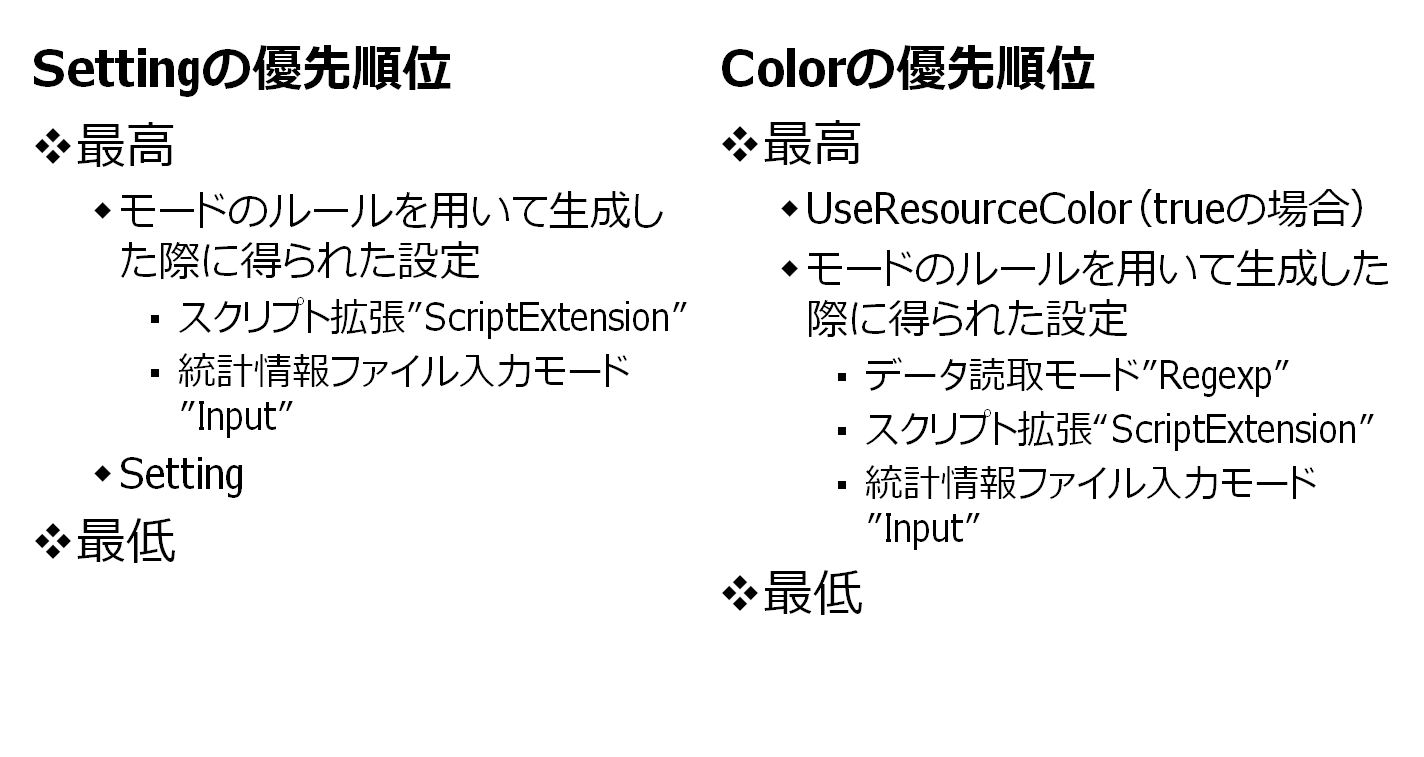
\includegraphics[scale=0.5]{settingpri.png}
\caption{�O���t�ݒ�̗D�揇��}
\label{fig:settingpri}
\end{center}
\end{figure}

{\tt "Setting"}�́C�������[�h�ɂ���ē��v���t�@�C����������ꍇ������̂�
�D�揇�ʂ��‚���K�v������D\sref{sec:inputmode}�ł��q�ׂ��悤�ɁC�������[�h��
����ē��v���t�@�C����������ꍇ�C����ꂽ���v���t�@�C���ɂ͓��v��񐶐����[��
�Œ�`�����ݒ�����œK�ȃO���t�ݒ肪����Ă���”\���������D�Ȃ��Ȃ�C���v��񐶐�
���[���ɒ�`����O���t�̐ݒ�́C�ύX�񐔂̌y�������邽�߂ɔėp���̍����ݒ肪�]��
��邩��ł���D����āC�}�̂悤�ȗD�揇�ʂƂ����D

�������[�h�ɂ����{\tt "Color"}���ݒ肳���ꍇ������̂ŁC{\tt "Color"}�ɂ��D��
���ʂ��‚���K�v������D�D�揇�ʂ́C{\tt "Setting"}�Ƃ͋t�̂悤�Ȍ`�ɂȂ��Ă���D����́C
���\�[�X�̐F���֌W���邩��ł���D���\�[�X�t�@�C���Œ�`����郊�\�[�X�̐F�́C
TLV�̉Ž����\�����ɕ\������ۂɎg�p�����ꍇ������D����𓝌v���\���@�\�ł�
���p�ł���悤�ɂ��邱�ƂŁC�F�ɂ�郊�\�[�X�̎��ʂ��”\�ɂ��C�O���t��ǂ݂₷��
�Ȃ�悤�H�v�����D����\verb|ON/OFF|���������Ă���̂�{\tt "UseResorceColor"}��
����D����́C{\tt "UseResorceColor"}��{\tt "true"}�ɂ���̂́C���[�U������
�悤�Ȍ��ʂ�_���Ă���”\������������ł���D����āC�}�̂悤�ȗD�揇�ʂƂ����D


\subsection{���v�����O���t�\�����邽�߂�GUI}
�{�߂ł́C���v���\���@�\�̎����ɔ����Ēlj����ꂽ2��ނ̃E�B���h�E�ɂ‚��Đ�������D�Y������E�B���h�E�́C���v�����O���t�\�����铝�v���r���[�A�ƃ��[�U���\�������铝�v����I�����铝�v���G�N�X�v���[���ł���D���\figref{fig:window}�Ɏ����D

\begin{figure}[ht]
\begin{center}
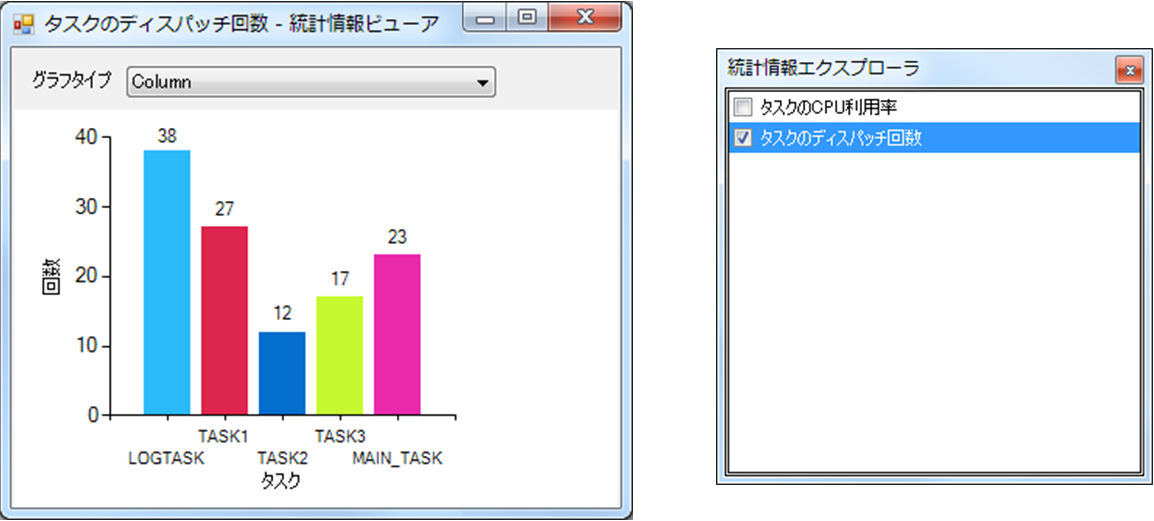
\includegraphics[scale=0.6]{window.png}
\caption{���v���r���[�A(��)�Ɠ��v���G�N�X�v���[��(�E)}
\label{fig:window}
\end{center}
\end{figure}

\subsubsection{���v���r���[�A}
���v���r���[�A�́C1�‚̃E�B���h�E��1�‚̃O���t��\������D�قȂ��ނ̃O���t�ŕ\���������Ƃ��̂��߂ɁC�O���t�̎�ނ��ȒP�ɐ؂�ւ�����@�\���������Ă���D�܂��C�E�B���h�E�̃T�C�Y��ς��邱�ƂŁC�O���t�̊g��k�����”\�ł���D

���̃E�B���h�E�́C���̃E�B���h�E���Ⴂ�CTLV�̃��C���E�B���h�E�Ƀh�b�L���O���ł��Ȃ��悤�ɂȂ��Ă���D���̃E�B���h�E�Ɠ����悤�Ɏ������Ă��܂��ƁC\figref{fig:tlvview}�Ɏ����E�B���h�E�̃��X�g�ɃE�B���h�E�����񋓂���邱�ƂɂȂ�D���v���t�@�C���́C1�‚̃��O�ɑ΂��ĕ����������邱�Ƃ��”\�ł���̂ŁC���̃��X�g�����p���Â炭�Ȃ�D

\begin{figure}[ht]
\begin{center}
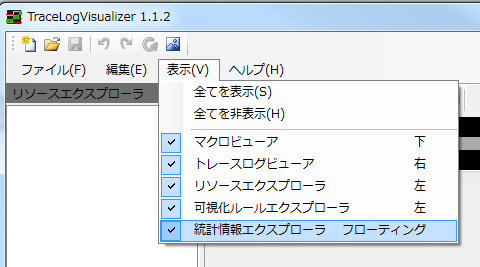
\includegraphics[scale=0.6]{tlvview.png}
\caption{�h�b�L���O�”\�ȃE�B���h�E�����X�g�A�b�v����Ă���Ƃ���}
\label{fig:tlvview}
\end{center}
\end{figure}

�O���t��\�������镔���̎����ɂ‚��ďq�ׂ�D�O���t��`�悷�邽�߂̃��C�u�����𒲍��������C.NET\ Framework\ 3.5�̕W�����C�u�����Ƃ��ėp�ӂ���Ă��炸�C���[�U���ɂ��J�����ɂ��V���Ƀ��C�u�������C���X�g�[������K�v���������D���̃��C�u�����́C.NET\ Framework\ 3.5�̒lj����C�u������.NET\ Framework\ 4��2��ނ���C���ꂼ��̓������������ēK�؂ȕ���I�������D

.NET\ Framework\ 3.5�̒lj����C�u�����́CMicrosoft\ Chart\ Controls\ for\ Microsoft\ .NET\ Framework\ 3.5�����[�U�����J�������C���X�g�[������K�v������D����́C.NET\ Framework�̃o�[�W�����A�b�v�ɂ��R�[�h���ς�s������Ȃǂ��s�킸�ɍςށD�������Ȃ���C���̃��C�u�����𗘗p����P�[�X��TLV�ȊO�ɂ��܂�l����ꂸ�CTLV�̂��߂����ɃC���X�g�[�����邱�ƂɂȂ肩�˂Ȃ��D

����C.NET\ Framework\ 4�ł́C�O���t��`�悷�郉�C�u�������W�����C�u�����Ƃ��ėp�ӂ���Ă���D����āCTLV�ȊO�ŕs�v�ƂȂ肤�郉�C�u�������C���X�g�[������K�v���Ȃ��D�܂��C���݂�TLV��Microsoft\ Parallel\ Extentions\ to\ .NET\ Framework\ 3.5�Ƃ���Community\ Technology\ Preview�C�‚܂�e�X�g�ł𗘗p���Ă��邪�C����ɂ‚��Ă��W�����C�u�����Ƃ��ėp�ӂ���Ă���D.NET\ Framework\ 3.5��.NET\ Framework\ 4�ł͌݊��������S�łȂ��̂ŁC�s�������J���‹��̍č\�z���s���K�v�����邪�C�O�q�������_�ɉ����C�J�����i�ނɂ‚�Ă������.NET\ Framework\ 4�ֈڍs����K�v���łĂ���ƍl���C.NET\ Framework\ 4�Ŏ������邱�Ƃɂ����D


\subsubsection{���v���G�N�X�v���[��}
���v���G�N�X�v���[���́C�\�������铝�v����I�����邽�߂̃E�B���h�E�ł���D������g�p���邱�ƂŁC���������v���Ɋւ��铝�v���r���[�A�݂̂�\�������邱�Ƃ��”\�ɂȂ�D

���̑��̖����Ƃ��āC�R���s���[�^�ƃ��[�U�ɂ����镉�ׂ̌y��������D�g���[�X���O�̉Ž��������̏I����C�S�Ă̓��v���r���[�A�𓯎��ɗ����グ�Ă��܂��ƁC�R���s���[�^�ɕ��ׂ�������CTLV�̉��������ቺ����D���̂����C���[�U�ɂƂ��ĕs�v�ȓ��v���r���[�A�܂ŗ����オ��”\��������D����āC�ŏ��͓��v���r���[�A�̃C���X�^���X�������C�K�v�ɂȂ������ɏ��߂ăC���X�^���X�����ĕ\�����邱�ƂŁC�����̖��������ł���D�܂��C�C���X�^���X���������̂́C�v�[�����O���邱�ƂŁC���̌�̃E�B���h�E�J�‚��~���ɍs����悤�ɂ����D


\section{���v���\���@�\�̎g�p����}
�{�߂ł́CTOPPERS/ASP�J�[�l��\cite{asp}�̃g���[�X���O�ɂ����铝�v���\���@�\�̗��p���
2�ʂ莦���C���v���\���@�\�̗L�p���ɂ‚��ďq�ׂ�D

��Ŏg�p����TOPPERS/ASP�J�[�l���̃g���[�X���O�́CTLV�̃p�b�P�[�W���Ɋ܂܂��T���v���ł���asp\_short.log�ł���D���̃��O�̃��\�[�X�t�@�C��asp\_short.res�ɂ́C�^�X�N�Ƃ��āC
LOGTASK�CTASK1�CTASK2�CTASK3�CMAIN\_TASK����`����Ă���D���̃��\�[�X�t�@�C���ɑ΂��āC
��Ɏ���2�‚̓��v��񐶐����[�����w�肷��D
�g���[�X���O���Ž������C�^�X�N�Ɋւ��Ă̂ݕ\���������̂�\figref{fig:aspsample}�Ɏ����D

\begin{figure}[ht]
\begin{center}
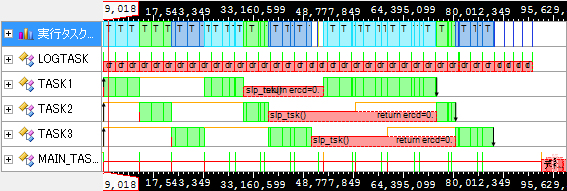
\includegraphics[scale=0.6]{asp_sample.png}
\caption{��Ɏ���TOPPERS/ASP�J�[�l���̃g���[�X���Oasp\_short.log�̉Ž���}
\label{fig:aspsample}
\end{center}
\end{figure}


\subsection{��{��̓��[�h��p�����e�^�X�N�̃f�B�X�p�b�`�񐔂̐���}
TOPPERS/ASP�J�[�l���ɂ�����e�^�X�N�̃f�B�X�p�b�`�񐔂́C�^�X�N�����s���(RUNNING)�ɂȂ�C�x���g�𐔂��邱�Ƃŋ��߂邱�Ƃ��ł���D�W���`���g���[�X���O�ŕ\����{\tt "Task.state=RUNNING"}�ł���C{\tt "Task"}�̕����Ɋe�^�X�N�������������O�𐔂��邱�Ƃœ��v���𐶐��ł���D
����āC��{��̓��[�h�𗘗p����ꍇ�C���v��񐶐����[���t�@�C����\sref{sec:statsgenfile}�Ŏ������}\ref{statsGenRule}�̂悤�ɂȂ�D�����̐������[�h�ɑ΂��郋�[�����L�q����Ă��Ă��C{\tt "Mode"}��{\tt "Basic"}���w�肷�邱�ƂŁC��{��̓��[�h�𗘗p�ł���D���̃t�@�C���ɒ�`�������v��񐶐����[��\verb|"task_dispatch_count"|��p���ē��v���𐶐����C�O���t�\���������̂�\figref{fig:aspsampledis}�Ɏ����D�O���t�̐F��\figref{fig:aspsample}�̎��s�^�X�N�̃��C���ɂ���}�`�̐F���r����ƁC�����悤�Ȓl�ɂȂ��Ă��邱�Ƃ��킩��D���ꂪ{\tt "UseResourceColor"}��{\tt true}�ɂ����Ƃ��̓���ł���D\figref{fig:aspsample}�̕��������̂́C�F�̃A���t�@�l���ʂ̒l�ɐݒ肳��Ă��邽�߂ł���D

���̓��v�������̋@�\�𗘗p�������߂�ꍇ�C\figref{fig:aspsample}�̊e�^�X�N�̃��C���ɕ\������Ă���ΐF�̒����`�������オ��ӏ������ƂŐ�������C�g���[�X���O�ɑ΂��Ċe�^�X�N����grep���s�����肷��K�v������D����ɁC���v�����O���t�\�����邽�߂ɂ́C���肵�����v�����O���t�쐬�c�[���֓��͂���K�v������D

\begin{figure}[ht]
\begin{center}
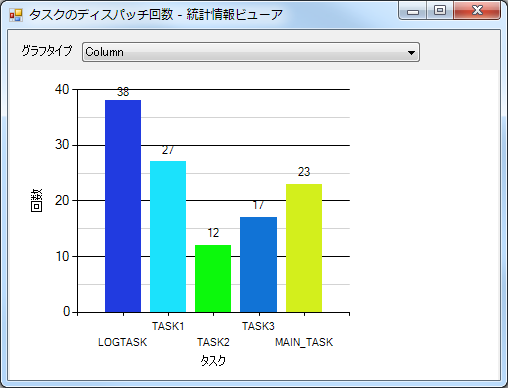
\includegraphics[scale=0.6]{aspsampledis.png}
\caption{asp\_short.log�ɂ�����e�^�X�N�̃f�B�X�p�b�`�񐔂̃O���t�\��}
\label{fig:aspsampledis}
\end{center}
\end{figure}

\subsection{�X�N���v�g�g�����[�h��p�����e�^�X�N��CPU���p���̐���}
TOPPERS/ASP�J�[�l���ɂ�����e�^�X�N��CPU���p���́C�^�X�N�����s��Ԃł��鎞�Ԃ����߁C���̎��Ԃ��g���[�X���O�̋L�^���ԂŊ��邱�Ƃŋ��߂邱�Ƃ��ł���D���s��Ԃł��鎞�Ԃ́C�^�X�N�̏�Ԃ����s��ԂɑJ�ڂ��Ă���C���̏�ԂɑJ�ڂ���܂ł̎��Ԃŋ��߂邱�Ƃ��ł��CCPU���p�����o���ɂ́C���̍��v�����߂�K�v������D�܂��C�g���[�X���O�̋L�^���Ԃ́C�g���[�X���O�̍Ō�̃��O�̎��Ԃ���ŏ��̃��O�̎��Ԃ��������Ƃŋ��߂邱�Ƃ��ł���D

�ȏ�̂悤�ɁC�l�X�Ȓl�𓱏o���C���������Z���邱�Ƃ́C��{��̓��[�h�ł̓T�|�[�g���Ȃ��D���̂悤�ȕ��G�Ȍv�Z��v���铝�v���ɂ́C�X�N���v�g�g�����[�h�𗘗p����D�e�^�X�N��CPU���p���𐶐����ē��v���t�@�C���Ƃ��ďo�͂���Ruby�X�N���v�gcpu\_utilization.rb��p�ӂ��C���v��񐶐����[���t�@�C���ɒ�`�������̂�}\ref{statsgenscr}�Ɏ����D���̃X�N���v�g�́C�ėp�����������邽�߁C�W���`���g���[�X���O����������D

\begin{figure}[h]
\begin{lstlisting}
{
  "cpu_utilization" : {
    "Setting":{
      "Title":"�^�X�N��CPU���p��",
      "AxisXTitle":"�^�X�N",
      "AxisYTitle":"����[%]",
      "DefaultType":"Pie"
    },
    "UseResourceColor":true,
    "Mode":"Script",
    "ScriptExtension":{
      "Target":"standard",
      "FileName":"c:/cygwin/bin/ruby",
      "Arguments":"F:/TLV/statisticsGenerationScript/cpu_utilization.rb"
    }
  }
}
\end{lstlisting}
\caption{cpu\_utilization.rb�𗘗p�������v���t�@�C���̐���}
\label{statsgenscr}
\end{figure}

���̃t�@�C���ɒ�`�������v��񐶐����[��\verb|"cpu_utilization"|��p���ē��v���𐶐����C�O���t�\���������̂�\figref{fig:aspsamplecpu}�Ɏ����D
�l���㉺2�i�ɂȂ��Ă��邪�C��̒l�����߂����v���ł���C���̒l���~�O���t�������Ƃ��̊�����\���Ă���D���̂悤�ɁC�O���t�ɂ���āC�K�؂ȕ\�����@������D�܂��C�e�^�X�N��CPU���p�����~�O���t�ŕ\�����̂ɂ�������炸�C�㉺�̒l����v���Ȃ��̂́C�S�̂̃A�C�h�����Ԃ̊������܂߂Ă��Ȃ����߂ł���D���̏�CLOGTASK��MAIN\_TASK�̒l�����������ďd�Ȃ��Ă��܂��Ă���D���̂悤�ȁC�O���t�̎�ނ�ύX���ĕ\���������ꍇ�C���v���r���[�A�̏㕔�ɂ���O���t�^�C�v�ƃ��x�����O���ꂽ�R���{�{�b�N�X�𑀍삷�邱�ƂŁC�O���t�̎�ނ�ύX�ł���D���_�O���t�ɕύX�������\figref{fig:aspsamplebar}�Ɏ����D

\begin{figure}[ht]
\begin{center}
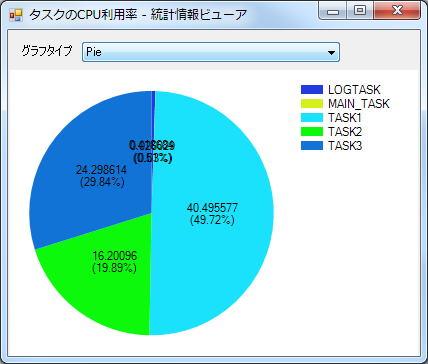
\includegraphics[scale=0.45]{aspsamplecpu.png}
\caption{asp\_short.log�ɂ�����e�^�X�N��CPU���p���̃O���t�\��(�������)}
\label{fig:aspsamplecpu}
\end{center}
\end{figure}

\begin{figure}[ht]
\begin{center}
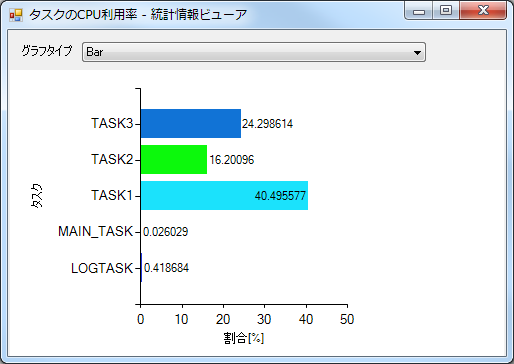
\includegraphics[scale=0.45]{aspsamplebar.png}
\caption{asp\_short.log�ɂ�����e�^�X�N��CPU���p���̃O���t�\��(�O���t�^�C�v�ύX��)}
\label{fig:aspsamplebar}
\end{center}
\end{figure}
\chapter{�g���[�X���O�p�[�T��\\���t�@�N�^�����O}\label{ch:refact}
\section{�T�v}
\subsection{���{���R}
�W���`���g���[�X���O�̃p�[�X�ɂ����āC
�}\ref{rex}�̂悤�ȕ��G�Ȑ��K�\�����v8��K�p���Ă���D����́CObject�Ȃǂ̗v�f1�‚ɂ‚�1�s�̐��K�\����
�擾���邽�߂ł���D�������邱�ƂŁCTime��Value���̗L���Ɋւ�炸
\footnote{�Ž������[���t�@�C���ɂ́CTime���Ȃ��CValue���Ȃ��CAttributeName���Ȃ����Ƃ�����
�s���S�ȕW���`���g���[�X���O���L�q����Ă���D}
�p�[�X�ł���悤�ɂ��Ă���D
�������C���̂悤�ȕ��G�Ȑ��K�\���͉“ǐ����Ⴂ�̂ŁC���t�@�N�^�����O�����{����D

���t�@�N�^�����O���TLV�́C�W���`���g���[�X���O�̃p�[�X���p�̃p�[�T�ɔC����D
�p�[�T���\������R�[�h���C\sref{sec:log}
�Ɏ���EBNF�̂悤�ɋL�q���邱�ƂŁC�J���҂��\���𒼊��I�ɗ����ł���悤�ɂȂ�D
�R�[�h���}\ref{refacted}�Ɏ����D

�܂��C�d�������R�[�h����ѐ����K���ύX���̕ύX�ӏ������炷���Ƃ��ł��邽�߁C�ێ琫�����シ��D
�Ⴆ�΁CTime���͂ދL��\verb!"[","]"!��\verb!"<",">"!�ɂ���Ƃ��C�]���̐��K�\����p����
���@�ł́C8�s���ׂĂ̐��K�\����ύX����K�v�����邪�C���t�@�N�^�����O���1�ӏ��ōςނ悤�ɂȂ�D
�����K����lj�����ꍇ�ł��C�]���̎�@�ł�8�s�̐��K�\���̒�����ύX�ӏ���T���˂΂Ȃ�Ȃ����C
���t�@�N�^�����O��́CEBNF�̂悤�ɋL�q����Ă��邽�߁C�ύX�ӏ������m�ł���̂Ō����Ƃ������点��D
�������Ȃ���C���̂悤�ȍ\���̕ύX�͋H�ł��邽�߁C��Ԃ̃����b�g�͍\���𒼊��I�ɗ����ł���悤�ɂȂ�
���Ƃł���D

\begin{figure}[h]
\begin{lstlisting}
m = Regex.Match(_log, 
      @"^(\[[^\]]+\])?(?<objectType>[^\[\]\(\)\.]+)\([^\)]+\)(\.[^\s]+)?$");

if (m.Success)
	ObjectType = m.Groups["objectType"].Value;
HasObjectType = m.Success;
\end{lstlisting}
\caption{���t�@�N�^�����O�O�̃R�[�h��}
\label{rex}
\end{figure}

\begin{figure}[h]
\begin{lstlisting}
var object_ = 
	ObjectTypeName().Char('(').AttributeCondition().Char(')')
	.OR().
	ObjectName();
\end{lstlisting}
\caption{���t�@�N�^�����O��ɕ\���������R�[�h��}
\label{refacted}
\end{figure}



\subsection{�Ώ�}\label{sec:tl}
���t�@�N�^�����O�Ώۂ́C\verb!TraceLog!�N���X�C���ɂ��̃R���X�g���N�^�ł���D
����\verb!TraceLog!�N���X�́C�W���`���g���[�X���O���\������g�[�N����ێ����C
�W���`���g���[�X���O��p����������e�Ղɂ���D

���݁C�W���`���g���[�X���O�̃p�[�X�ɐ��K�\����p���Ă���ӏ���
�p�[�T��p����悤�ɁC\verb!TraceLog!�R���X�g���N�^��ύX����D


\newpage
\subsection{�ύX���e}
\subsubsection{�N���X�\��}\label{sec:refclass}
\verb!Regex!�N���X��\verb!Match!�N���X��p�������K�\���ɂ��p�[�X��p�~���C
�W���`���g���[�X���O�p�̃p�[�T���쐬����D�����āC\verb!TraceLog!�N���X�́C���̃p�[�T�փp�[�X�������Ϗ�����D
����ɂ��C���݂̓p�[�X�̎�����\verb!TraceLog!�N���X�ɒ���������Ă��邽��
�p�[�X�̎������@��ύX����̂�����ł���̂��C
\verb!TraceLog!�N���X�ƃp�[�X�̎����𕪗����邱�ƂŃp�[�T�̌������e�ՂɂȂ�C
�p�[�T�̎������@�ύX���e�ՂɂȂ�D

����̕ύX�ɔ����e���͈͂́C\verb!TraceLog!�N���X�ȊO�ɑ��݂��Ȃ��D
���t�@�N�^�����O�O��̃N���X�}��}\ref{bclass},\ref{aclass}�Ɏ����D

\begin{figure}[H]
\centering
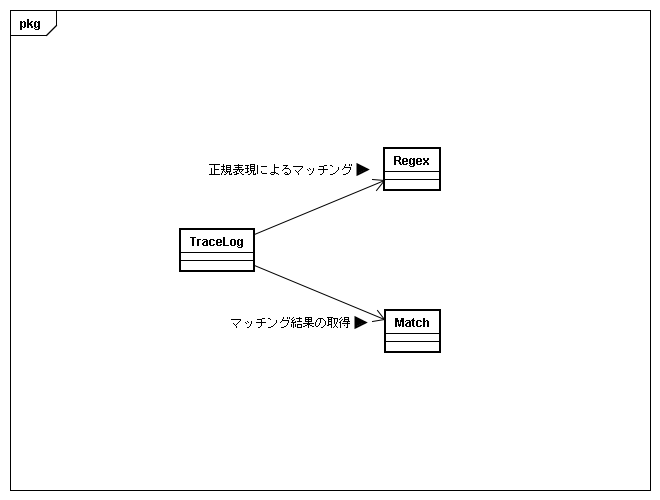
\includegraphics[scale=0.5]{bclass.png}
\caption{���t�@�N�^�����O�O�̃N���X�\��}\label{bclass}
\end{figure}

\begin{figure}[H]
\centering
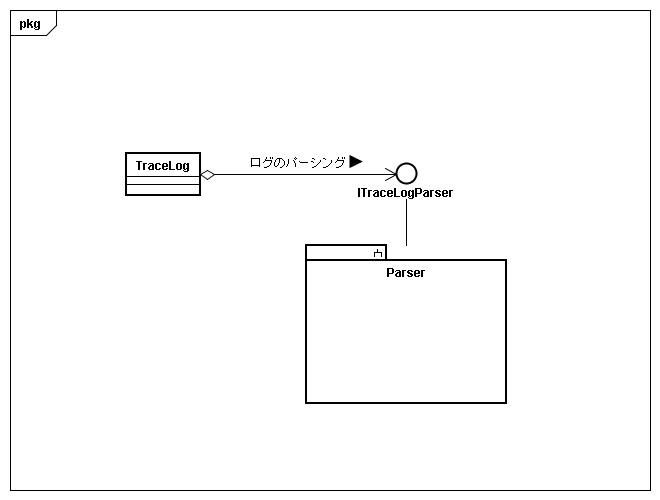
\includegraphics[scale=0.5]{aclass.png}
\caption{���t�@�N�^�����O��̃N���X�\��}\label{aclass}
\end{figure}


% \subsubsection{�����̗���}
% ���t�@�N�^�����O�O�̏����̗���́C�}\ref{before}�̂悤�ɁC
% \verb!TraceLog!�R���X�g���N�^�ɂĐ��K�\����p�����p�[�X���s���Ă���D

% ���t�@�N�^�����O��̏����̗���́C�}\ref{after}�̂悤�ɁC
% \verb!TraceLog!�R���X�g���N�^�Ńp�[�T�N���X�̃��\�b�h���ĂсC
% �p�[�T�N���X�ɂĕW���`���g���[�X���O�̃p�[�X���s���D
% �p�[�X���I��������C�p�[�T�N���X���猋�ʂ��󂯎��C�e�l��ݒ肷��D

% \begin{figure}[H]
% \centering
% 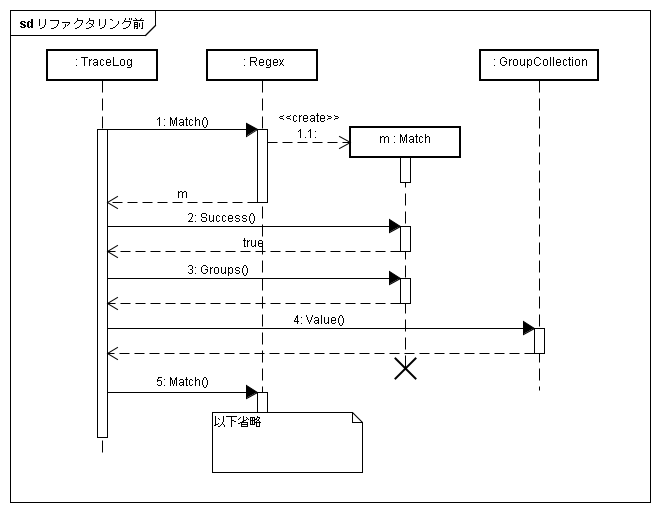
\includegraphics[scale=0.6]{before.png}
% \caption{���t�@�N�^�����O�O�̕W�����O�ϊ�����}\label{before}
% \end{figure}

% \begin{figure}[H]
% \centering
% 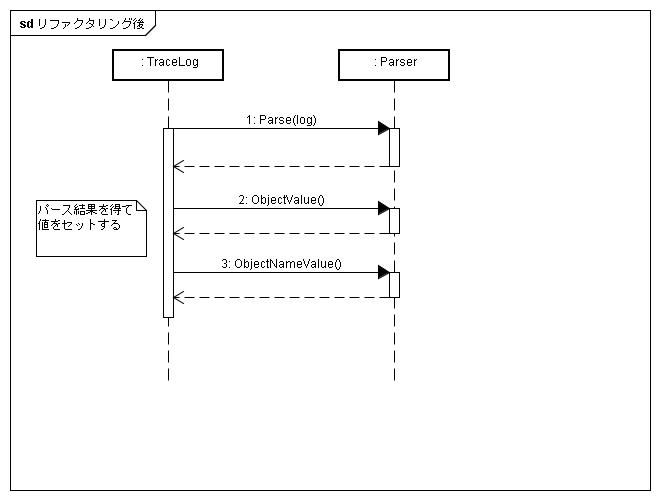
\includegraphics[scale=0.6]{after.png}
% \caption{���t�@�N�^�����O��̕W�����O�ϊ�����}\label{after}
% \end{figure}


\subsubsection{�p�[�T�̍\��}\label{sec:parsec}
�p�[�T�̎����́C�R�[�h��EBNF��\�����C�����I�ɗ����ł���悤�ɂ���D

��Ƃ��āCHaskell�̃p�[�T�R���r�l�[�^���C�u����Parsec���Q�l�ɂ����p�[�T\cite{parsec}����������D
���̃R�[�h���g�p���邩�C����ȂǑ��̎������@��p���邩�́C
�f�o�b�O�̗e�Ղ��C�����̂��₷���C�“ǐ��C���s���x�Ȃǂ̗v�f�ɂ�茈�肷��D


\newpage
\section{�ڍ׎d�l}\label{sec:refspec}
�{�߂́C�t�F�[�Y5�ōs�������t�@�N�^�����O�ɂ��ύX�E�lj����ꂽ�ӏ��C����сC
���t�@�N�^�����O��̃V�[�P���X��������C����̗p���Ȃ�������@�Ƃ̔�r�⍡��̎����̗̍p���R���L�q����D


\subsection{�R�[�h�݌v}
�����ł́C���t�@�N�^�����O�̖ڕW�ł������CEBNF��\�����Ē����I�ɗ����ł���R�[�h�̏Љ�ƁC
���߂ɂĎ����ɗp������@�E�T�O����ю�v���\�b�h�̐���������D

�܂��CEBNF��\�������R�[�h�̗��}\ref{code1}�Ɏ����D

\begin{figure}[h]
\begin{lstlisting}
var line = Char('[').Time().Char(']').Event();
...
var object_ = 
	ObjectTypeName().Char('(').AttributeCondition().Char(')')
	.OR().
	ObjectName();
...			
var typeName = Many1(() => AnyCharOtherThan('(', ')', '.'));
\end{lstlisting}
\caption{�R�[�h��EBNF��\�������R�[�h��}
\label{code1}
\end{figure}


����́C����EBNF���p�[�X���邱�Ƃ������Ă���D

\begin{figure}[h]
\begin{lstlisting}
TraceLogLine = "[", Time, "]", Event;

Resource = ResourceTypeName, "(", AttributeCondition, ")"
	 | ResourceName;

ResourceTypeName = /[0-9a-Z_]+/;
\end{lstlisting}
\caption{�}\ref{code1}���\�����ۂ�EBNF}
\label{ebnf1}
\end{figure}


���̂悤�ɁC�}\ref{code1}��EBNF��\�����Ă���C���K�\���ɂ��p�[�V���O���“ǐ���
���サ�Ă���D�}\ref{code1}�́C���ۂɂ͐}\ref{code2}
�̂悤�ȉ�̓��\�b�h���ɋL�q����C�����g�ݍ��킹�邱�ƂŐ}\ref{code1}���������Ă���D
\clearpage
\begin{figure}[h]
\begin{lstlisting}
public ITraceLogParser ObjectTypeName()
{
	Begin();

	var typeName = Many1(() => AnyCharOtherThan('(', ')', '.'));

	typeName.ObjectTypeValue = Result();
	return (ITraceLogParser)typeName.End();
}
\end{lstlisting}
\caption{��̓��\�b�h��}
\label{code2}
\end{figure}

\subsubsection{���p�����T�O�E��@}
�{�߂ł́C���p�����T�O�Ǝ�@�ɂ‚��ďq�ׂ�D
\begin{description}
\item[�ċA���~�p�[�T] \mbox{} \\
����C���������p�[�T�́C�X�^�b�N�𗘗p�����ċA���~�p�[�T�ł���C�o�b�N�g���b�L���O��p���Ă���D
����́CEBNF�̂悤�Ƀg�b�v�_�E���ɋL�q����Ă�����̂�\������̂ɓK���Ă��邪�C
�o�b�N�g���b�L���O�ɂ�鏈�������ቺ�����O�����D

\item[�p�[�T�E�R���r�l�[�^] \mbox{} \\
�p�[�T�E�R���r�l�[�^�Ƃ́C�p�[�T�ƃp�[�T��g�ݍ��킹�邱�Ƃ̂ł���R���r�l�[�^���w���D
��̓I�ɂ́CMany���\�b�h�CMany1���\�b�h�COR���\�b�h����������D
����ɂ��CEBNF�̕\����LL(k)���@�̃p�[�V���O���”\�ɂ��Ă���D
�������Ȃ���CLL(k)���@���������ߐ����K�����獶�ċA���̏������K�v�ł���D

\item[NullObject�p�^�[��] \mbox{} \\
�C���^�t�F�[�X���������Ă��邪�C�������Ȃ��N���X��p����f�U�C���p�^�[���ł���D
���Ԑ��𗘗p�������̂ŁCNull���ǂ����𔻕ʂ���R�[�h��r���ł��C�����̗��ꂪ���m�ɂȂ�D
����C�����p���邱�Ƃ�EBNF�̂悤�ȋL�q���������Ă���D
��̓��\�b�h�́C�p�[�T�N���X�������̓p�[�T�N���X�p��NullObject��Ԃ����ƂŎ��̉�̓��\�b�h�����s���邩�����肷��D
����ɂ��Cif�����͂��܂��Ƀ��\�b�h�`�F�[���݂̂Ő����K����\���ł���悤�ɂȂ�D
���ɁC�Ӑ}���Ȃ�Null�Q�Ƃɂ���O�����Ȃǂ́CNull�ɂ�����h�~�ł���Ƃ��������b�g������D
\end{description}

\subsubsection{��{���\�b�h�̐���}\label{sec:ms}
�{�߂ł́C�p�[�T���L�q�����Ŋ�{�ƂȂ郁�\�b�h�ɂ‚��ďq�ׂ�D
\begin{description}
\item[Begin���\�b�h] \mbox{} \\
��̓��\�b�h�̏����ōŏ��Ɏ��s����郁�\�b�h�ł���D

���݂́C�X�^�b�N�ւ̃p�[�X���ʂ���у|�C���^
\footnote{�p�[�V���O���̕�����́C��͂̌��݈ʒu(����)���������́D}
�̕ۑ��̈�m�ۂ��s���Ă���D

\item[End���\�b�h] \mbox{} \\
��̓��\�b�h�̏����ōŌ�Ɏ��s����郁�\�b�h�ł���D
��{�I�ɁC�p�[�X�����s�C�‚܂�C�����K����\�����\�b�h�`�F�[�������s���ē���ꂽ�߂�l
�ł���p�[�T�I�u�W�F�N�g�܂���NullObject����Ă΂��D
���݂́C�X�^�b�N�̃|�b�v�C���O�̃X�^�b�N�ɂ���p�[�X���ʂƂ̌����CNullObject�̃X�e�[�^�X���������s���Ă���D
�p�[�T�N���X��NullObject�N���X���œ��삪�ς��D

\item[Result���\�b�h] \mbox{} \\
�p�[�X�����s���ē���ꂽ�������Ԃ����\�b�h�ł���D

\item[OR���\�b�h] \mbox{} \\
EBNF�̋L��\verb!"|"!��\�����\�b�h�ł���D�����K����\�����\�b�h�`�F�[���Ŏg�p����D
���̃��\�b�h���O�̐����K���ɓ��Ă͂܂�Ȃ������ꍇ�C���̃��\�b�h���Ńo�b�N�g���b�L���O���āC
���̐����K���̓K�p�����݂�D

\item[Many���\�b�h] \mbox{} \\
EBNF�̋L��\verb!"*"!��\�����\�b�h�ł���D�����K����\�����\�b�h�`�F�[���Ŏg�p����D
�����ɗ^����ꂽ��̓��\�b�h��0��ȏ�K�p������D

\item[Many1���\�b�h] \mbox{} \\
EBNF�̋L��\verb!"+"!��\�����\�b�h�ł���D�����K����\�����\�b�h�`�F�[���Ŏg�p����D
�����ɗ^����ꂽ��̓��\�b�h��1��ȏ�K�p������D
\end{description}

\subsection{�N���X�݌v}
���t�@�N�^�����O��̃N���X�}��}\ref{class}�Ɏ����D
\verb!TraceLog!�N���X�ȊO�̃N���X�Q���C\sref{sec:refclass}�̐}\ref{aclass}�ɂ���T�u�V�X�e���ɑ�������D

�p�[�T�́C��{�I�ȋ@�\��������N���X�ƃp�[�X�Ώۂɓ��������N���X�ɂ킯�邱�ƂŁC
��{�I�ȋ@�\��������N���X�̍ė��p���ł���悤�ɂȂ��Ă���D
���̂��߁C����ɊY������Parser�N���X�����NullObjectForParser�N���X��
�p������h���N���X���`���CITraceLogParser�N���X�̂悤�ȓ��������C���^�t�F�[�X���`���Ă��ꂼ���
�h���N���X���������邱�ƂŁC�l�X�ȃp�[�T���쐬�”\�ł���D

���ɁC�}\ref{class}�̊e�N���X�ɂ‚��Đ�������D

\begin{figure}[H]
\centering
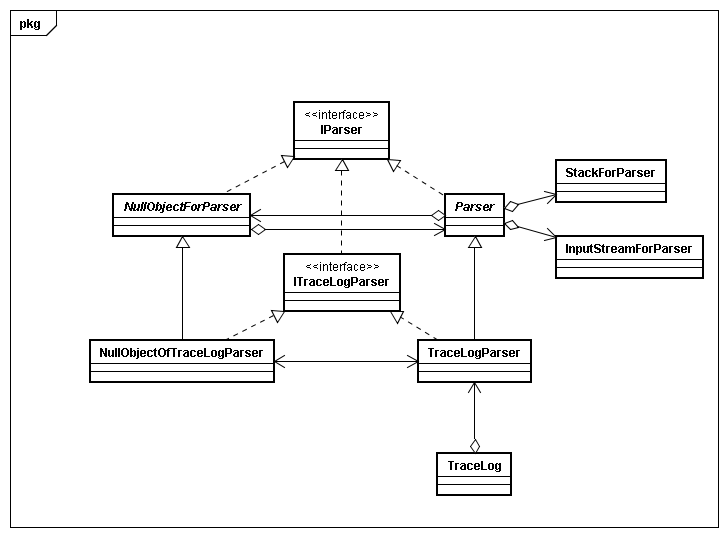
\includegraphics[scale=0.5]{class.png}
\caption{���t�@�N�^�����O��̏ڍׂȃN���X�\��}\label{class}
\end{figure}

\subsubsection{���݃N���X}
�{�߂ł́C���t�@�N�^�����O�ȑO���瑶�݂���N���X�ɂ‚��ďq�ׂ�D
\begin{description}
\item[TraceLog�N���X] \mbox{} \\
�W���`���g���[�X���O���R�[�h��ň������߂̃N���X�ł���D
����C���̃R���X�g���N�^�����t�@�N�^�����O���C�“ǐ��̌�����s�����D
�܂��C�V����\verb!TraceLogParser!�I�u�W�F�N�g��ێ�����ÓI�t�B�[���h��lj����C
�p�[�T�̐��������ōςނ悤�ɂ����D
\end{description}

\subsubsection{�V�݃N���X}
�{�߂ł́C���t�@�N�^�����O�ɂ��V�����lj������N���X�ɂ‚��ďq�ׂ�D
\begin{description}
\item[Parser�N���X] \mbox{} \\
�p�[�T���������邽�߂̊�{�I�ȋ@�\��������N���X�ł���D
������p�����C��̓��\�b�h���L�q���邱�ƂŐ�p�̃p�[�T���쐬����D
\ref{sec:ms}�Ɏ��������\�b�h�̑��ɁC�A���t�@�x�b�g�␔���̉�̓��\�b�h���L����D
�����̃��\�b�h�́C�P���Ɍp�����������ł͖߂�l�̌^�����킸�C�g�p�ł��Ȃ��D
����āC�h���N���X�ɁC������\verb!Parser!�N���X�ɈϏ����C���̌��ʂ��g�p����C���^�t�F�[�X�^�ɃL���X�g����\verb!return!����
����(�������́C����Ƃ킩�閼�O)�̃��\�b�h��p�ӂ��Ďg�p����D

\item[StackForParser�N���X] \mbox{} \\
\verb!Parser!�N���X�����p�����p�X�^�b�N�ł���D
�p�[�T�����܂ł̃p�[�X���ʂ�|�C���^��ޔ�������̂ɗp����D�ł��邾�������悭�Ǘ����邽�߂ɗp�ӂ����D

\item[InputStreamForParser�N���X] \mbox{} \\
�p�[�X�Ώۂ��i�[���C�Ǘ�����N���X�ł���D
�|�C���^�̐����|�C���^�̎��������̒񋟂Ȃǂ��s���D
\verb!.NET Framework!�̕W�����C�u�����ł���\verb!StringReader!�N���X�́C
Read���\�b�h�ŕ���������Ă��܂��ĕ�����������߁C��p�̃N���X��p�ӂ����D

\item[NullObjectForParser�N���X] \mbox{} \\
\verb!Parser!�N���X��NullObject���������邽�߂̊�{�I�ȋ@�\��������N���X�ł���D
������p�����C��̓��\�b�h���܂ރC���^�t�F�[�X���������邱�ƂŁC��p�̃p�[�T�pNullObject���쐬����D


\item[TraceLogParser�N���X] \mbox{} \\
�W���`���g���[�X���O�p�̃p�[�T�N���X�ł���D
�W���`���g���[�X���O���p�[�X���邽�߂̉�̓��\�b�h�⌋�ʂ��擾���邽�߂̃v���p�e�B������D

\item[NullObjectOfTraceLogParser�N���X] \mbox{} \\ %\label{sec:nullobj}
�W���`���g���[�X���O�p�̃p�[�T�N���X�p��NullObject�N���X�ł���D
���\�b�h�͊�{�I�ɉ������Ȃ����C������A���S���Y����̗��R�Ȃǂŏ������s���ꍇ������D
�������CNullObject�Ƃ��Ă͈ٗ�Ȃ��߁C���̂悤�ȏꍇ�͕ێ琫���ቺ���鋰�ꂪ����D

\item[IParser�N���X] \mbox{} \\
\verb!Parser!�N���X��\verb!NullObjectForParser!�N���X�����ԃC���^�t�F�[�X�ł���D
����ɂ��C���\�b�h�`�F�[���ɂ��EBNF�̂悤�ȕ\�����������Ă���D

\item[ITraceLogParser�N���X] \mbox{} \\
\verb!TraceLogParser!�N���X��\verb!NullObjectOfTraceLogParser!�N���X�����ԃC���^�t�F�[�X�ł���D
����ɂ��C���\�b�h�`�F�[���ɂ��EBNF�̂悤�ȕ\�����������Ă���D
\end{description}

\subsection{�V�[�P���X}
��Ƃ��āC\verb!"[.]Task.state=="RUNNING""!�Ƃ�����������O���p�[�X����
�V�[�P���X�̈ꕔ��}\ref{sequence}�Ɏ����D��̓��\�b�h�̓K�p�ɐ�������Ύ��̉�̓��\�b�h�����݁C
���s����Έȍ~�̉�̓��\�b�h��NullObject�̂��̂��ĂԂ��ƂŃp�[�T�̉�̓��\�b�h��K�p���Ȃ��悤�ɂȂ��Ă���D

�܂��C���s������Ԃ�OR���\�b�h���Ă΂��ƃo�b�N�g���b�N���COR���\�b�h�ȍ~�̉�̓��\�b�h�ɂ��ēx�p�[�X���s����D
���̑��̏�ԂŌĂ΂ꂽ����OR���\�b�h�̏�����}\ref{orsequence}�Ɏ����D
3�–ڂ̏ꍇ�́C�Ⴆ��\verb!hoge().OR().fuga().OR().piyo()!�Ƃ��������K�����������ꍇ�C
\verb!hoge()!��������������\verb!fuga()!��\verb!piyo()!�̊Ԃɂ���\verb!OR()!�̋�����
��������D

\begin{figure}[H]
\centering
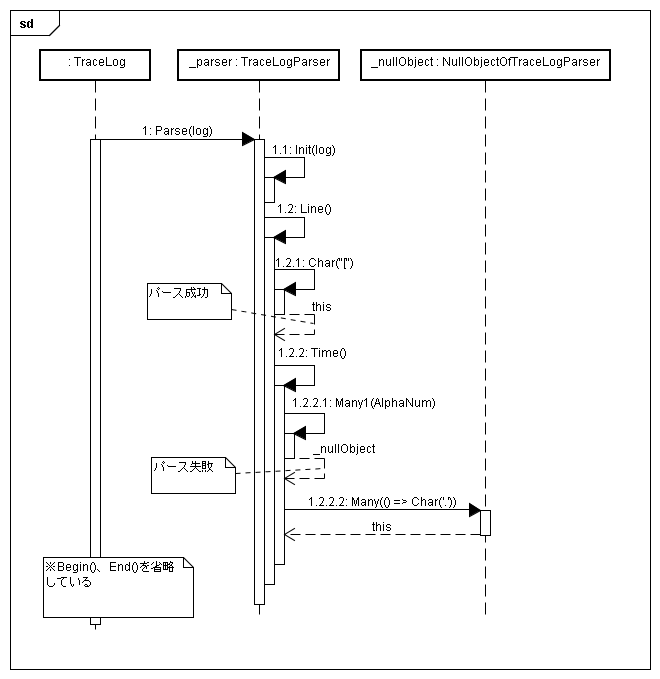
\includegraphics[scale=0.6]{sequence.png}
\caption{�p�[�V���O���̃V�[�P���X�̈ꕔ}\label{sequence}
\end{figure}

\begin{figure}[H]
\centering
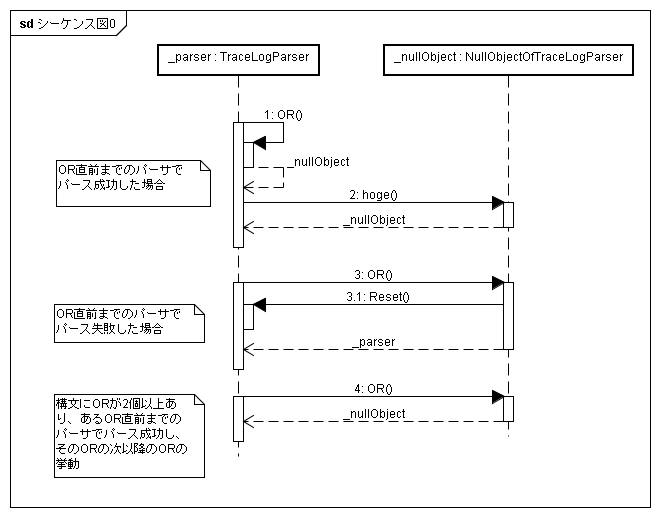
\includegraphics[scale=0.6]{orsequence.png}
\caption{�e��Ԃł�OR���\�b�h�̏���}\label{orsequence}
\end{figure}


\newpage
\section{�]��}
�{�߂́C\ref{sec:parsec}�ŏЉ��\cite{parsec}��p�����p�[�T(�ȍ~�CC\#��Parsec)�C\sref{sec:refspec}�ŏЉ���p�[�T(�ȍ~�C����p�[�T)���r���C
����p�[�T��I���������R���L�q����D
�܂��C������‚̃p�[�T����я]���̃p�[�X��@�Ő��\��r�������D

\subsection{�“ǐ�}
�܂��CC\#��Parsec�̃R�[�h��}\ref{codeparsec}�Ɏ����D
���̃p�[�T�́CHaskell��Parsec��͂����R�[�h�ɂȂ��Ă���C�}\ref{haskellcode}�̂悤�ɒu�������邱�Ƃ��ł���D
���Ȃ킿�C�}\ref{codeparsec}�ł́C\verb!in!���E�̉�̓��\�b�h���ォ�珇�Ɍ������̂������K����\���Ă���D
�������Ȃ���C���̋L�q�́C�R�[�h��ŃN�G�������L�q�ł���LINQ�𗘗p���Ă��邽�߁C
�����ł͗������ɂ����Ƃ������Ƃ����݂̊J�������o�Ƃ̃��r���[�ŏo�Ă����D�܂��C
�E�̉�̓��\�b�h���ォ�珇�Ɍ������̂������K����\���Ă��邱�Ƃ��킩�����Ƃ��Ă��C
\verb!select!����������̂��C�����L�q����Ă���̂����������ɂ����D
���̂��߁CHaskell�o���҂ł���΂悢�Ƃ͎v���邪�C�����łȂ��҂ɂƂ��Ă͉“ǐ����]���̂��̂��Ⴍ�Ȃ��Ă��܂�
�”\��������D

����p�[�T�́C�����K����\����̓��\�b�h�̃`�F�[����EBNF�ɋ߂����߁C����p�[�T�̕����“ǐ��������Ƃ������r���[����
������ꂽ�D

\begin{figure}[h]
\begin{lstlisting}
OBject = (from otn in ObjectTypeName
          from u1 in Char('(')
		  from ac in AttributeCondition
		  from u2 in Char(')')
		  select Base(otn).Append(u1).Append(ac).Append(u2).ToString())
		 .OR(
		 (from on in ObjectName
		  select Base(on).ToString()));
		  
// Base���\�b�h�́C�����Ɋ�Â���StringBuilder�N���X��V�K�쐬���ĕԂ����\�b�h
// StringBuilder�N���X�Ɋւ��ẮC.NET Framework ���C�u�������Q��
\end{lstlisting}
\caption{C\#��Parsec�̃R�[�h��}
\label{codeparsec}
\end{figure}
\clearpage
\begin{figure}[h]
\begin{lstlisting}
OBject = do{ otn <- objectTypeName
           ; u1 <- char '('
           ; ac <- attributeCondition
           ; u2 <- char ')'
           ; return�@$ otn ++ u1 ++ ac ++ u2
           }		   
         <|>
         do{ on <- objectName
           ; return $ on
           }
\end{lstlisting}
\caption{�}\ref{codeparsec}��Haskell�ɒu���������R�[�h��}
\label{codeparsec}
\end{figure}

\subsection{�ێ琫}
C\#��Parsec�̃N���X�\���́C�@�\���Ƃɂ悭�����E��������Ă���C�܂��C������ȊO�ɂ��Ή��ł���悤��
�݌v����Ă��邽�ߔėp���������D
����C\#��Parsec����уp�[�T��ύX����ɂ́CParsec�̎����Ɋւ���m�����K�v�ɂȂ�D
����ɔ����CHaskell�̒m�����K�v�ɂȂ�ꍇ������D
����āC�`���[�j���O�܂ōs�����Ƃ���ƁC���O�m�����Ȃ���Ίw�K�R�X�g���������Ă��܂��D

����p�[�T�́C������̃p�[�V���O�ɓ����������̂ł���C�����񉻂ł��Ȃ����̂̃p�[�V���O�͂قڕs�”\�ɋ߂��D
�������Ȃ���CTLV�ŗp����ꍇ�C������ȊO�͌���ł͍l�����Ȃ����߁C���ɂȂ�Ȃ��D
�ύX����R�X�g�Ɋւ��ẮC����p�[�T�ł��CNullObject�Ƃ̘A�g���̓��\�b�h�̃`�F�[���̗����Ɋw�K�R�X�g��������D

���ɁC�����K���̕ύX�ɂ‚��čl����D
����ɂ‚��ẮC�����Ƃ�EBNF��\���������̂ł��邽�߁C��{�I�Ȏ菇������͓����ł���D
�L�q�ύX���ׂ��ӏ��́C�ړI�̐����K����\�����Ă���ӏ����݂�΂悢�̂ŁC
�]���̎�@���ύX�ӏ��𔭌����₷���C�ύX�ӏ��̌����팸�ł���D
�ύX�ɂ́C�����K���̒lj��C�폜������
\footnote{����ւ��́C�lj��E�폜��g�ݍ��킹�����̂ƍl�����邽�ߏ��O}
�̂ŁC���̏����Ō��Ă����D
�܂��lj����ɂ́C���̎菇�𓥂ށD
\begin{enumerate}
\item �V�K�̐����K���ɂ��������ĉ�̓��\�b�h���쐬����
\item �V�K�̉�̓��\�b�h�������̐����K���ɑ}������
\item C\#��Parsec�̏ꍇ�F�V�K�̉�̓��\�b�h��}�����������̐����K����select�������������
\end{enumerate}
�폜���ɂ́C���̎菇�𓥂ށD
\begin{enumerate}
\item �����̐����K������ړI�̉�̓��\�b�h���폜����
\item C\#��Parsec�̏ꍇ�F��̓��\�b�h���폜���������K����select�������������
\end{enumerate}
�ȏ�̂悤�ɁCC\#��Parsec�̏ꍇ�́C����p�[�T��葽���L�q���Ȃ���΂Ȃ�Ȃ��ꍇ������̂ŁC
�ύX�ӏ����ł����΁C����p�[�T�̕����D���ꍇ������D

\subsection{�f�o�b�O�̗e�Ր�}
C\#��Parsec�́C���Ȃ�̊������f���Q�[�g����߂�D���̂��߁C�f�o�b�K�ɂ��X�e�b�v���s�ł́C�ǂ̃f���Q�[�g��
�K�p����Ă���̂����킩��Â炭�C���ʁC�����̗��ꂪ�c�����Â炢���߃f�o�b�O������D�܂��C���ꎩ�̂������Ɗւ���Ă��邽�߁CParsec�Ȃǂ̒m�����K�v�ƂȂ�D

����p�[�T�́C�R�[�h����������f�o�b�K�ɂ��X�e�b�v���s���s���������f�o�b�O���e�Ղł���D
���ɁC�擾�������p�[�X���ʂ̊i�[���́C�}\ref{code3}�̃R�[�h�́�1�C2�ł���D

\begin{figure}[h]
\begin{lstlisting}
var object_ =
	ObjectTypeName().Char('(').AttributeCondition().Char(')')
	.OR().
	ObjectName();

object_.ObjectValue = Result();    // ��1

// HasObjectTypeValue�́CObjectTypeName()���^�ł��C�ق��Ŏ��s����΋U�ł���D
object_.HasObjectTypeValue = false;  // ��2
\end{lstlisting}
\end{figure}

�Ⴆ�΁�1�C2�́C\verb!object_!�������w���̂��𐄑����ċL�q����K�v������D
�f�o�b�K�ɂ��X�e�b�v���s���s�����ƂŁC\verb!object_!�����m�ƂȂ�C�������Ԉ���Ă��Ȃ����m�F�ł���D
�܂��CC\#��Parsec�̂悤�Ƀf���Q�[�g�𑽗p���Ă��炸�C�g�p���Ă��Ă��V���v���ȃV�[�P���X�ł��邽�߁C
�ǂ̃��\�b�h�܂��̓f���Q�[�g��K�p�����Ă���̂���C\#��Parsec���V�[�P���X��ǂ��₷���D

\subsection{���\��r}
\subsubsection{�������x}
�e��@�Ԃŏ������x�̈Ⴂ���o�邩�𒲍������D
TLV�́C���[�U���獂�����̗v���𒸂��Ă��邽�߁C�������x�����t�@�N�^�����O�ɂ�蒘�����ቺ���邱�Ƃ͖]�܂����Ȃ��C
�t�Ƀ��t�@�N�^�����O�ɂ�荂�������邱�Ƃ��]�܂����D

�ȉ��̕��@�ōs�����D
\begin{screen}
\begin{description}
\item[�p�������] �e�p�[�T����������TLV(�v3��)�C�X�g�b�v�E�H�b�`
\item[�v���J�n] �u�V�K�쐬�E�B�U�[�h�v�́uOK�v�{�^������������Ԃ��痣�����Ƃ�
\item[�v���I��] �u���������v�Ƃ������ɐ؂�ւ�����Ƃ�
\item[�v������] ����p�[�T3��C\#��Parsec3�񁨏]��3��
\item[����(.log)] 6958�s (TLV�t���̃T���v���t�@�C�� fmp\_long.log)
\item[����(.res)] ���\�[�X��28 (TLV�t���̃T���v���t�@�C�� fmp\_long.res)
\item[���l] 1��̑���ɂ‚�TLV�̋N���E�I�����s��
\end{description} 
\end{screen}


���{�‹��͎��̒ʂ�D
\begin{screen}
\begin{description}
\item[OS] Windows 7 Professional�@x64
\item[CPU] Core2Duo E8400(3.0GHz)
\item[������] DDR2-800�@1GBx2+2GBx2
\end{description} 
\end{screen}

���ʂ�\\ref{tb:result}�Ɏ����D

\begin{table}[H]
 \centering
 \caption{�������x�̑��茋��}�@\label{tb:result}
 \begin{tabular}{|c|c|c|c|} \hline
           &  1���&  2���&3���\\ \hline
����p�[�T   &2��26�b&2��21�b&2��22�b\\ \hline
C\#��Parsec&2��40�b&2��38�b&2��38�b\\ \hline
�]����@    &2��25�b&2��24�b&2��24�b\\ \hline
 \end{tabular}
\end{table}

���ʂ͎���p�[�T�C�]����@�CC\#��Parsec�̏��ł������D
����p�[�T�́C�������Ԃ�C\#��Parsec����11\%�C�]����@����2\%�Z���C
�������x�ʂł��D��Ă��邱�Ƃ��킩��D

����p�[�T������荂���ł��闝�R�́C���̂��̂��l������D
\begin{itemize}
\item ����������̂܂܈����̂ł͂Ȃ��C������𕶎��ɕ������ăR�X�g���Ⴂ�����������s��
\item ����p�[�T��p�̃X�^�b�N����ѓ��̓X�g���[���̂��ߖ��ʂ����Ȃ�
\item ������ɓ������邱�ƂŁC�����ȕ����񏈗����s����StringBuilder�N���X���̗p�ł���
\end{itemize}

C\#��Parsec�����̂悤�Ȍ��ʂɂȂ������R�́C���̂��̂��l������D
\begin{itemize}
\item �N���X���\�b�h�Ăяo�����R�X�g�̂�����f���Q�[�g�𑽗p���Ă���
\item �ėp�������߂邽�߂ɁC�v�f�̌�����z��̌���
\footnote{�z�񓯎m�̌����͕�����̌������R�X�g������}�ōs���Ă���(Parsec�̎����Ɏ����Ă���)
\item new�𑽗p���C�����̃C���X�^���X�����s���Ă���
\end{itemize}


\subsubsection{��͔\��} 
��͔\�͂́C3��ޑS�Ă̎�@�ŕς��Ȃ��D
����p�[�T�����C\#��Parsec��LL(K)���@����͂ł��C
�]���̎�@��.NET Framework�̐��K�\�����ʏ�̐��K�\�����_��‹��͂ɂł��Ă���\cite{msdn}���߁C
�W���`���g���[�X���O�̃p�[�V���O�ɖ��͂Ȃ�����ł���D
�������Ȃ���C�]���̎�@�Ŏg�p����Ă������K�\���ł́C
���ʂ̃l�X�g�𐳊m�Ƀp�[�X����̂ɁC����ȏ�ɕ��G�Ȑ��K�\���ƂȂ��Ă��܂�
\footnote{�]���̎�@�ł́C���ʂ̃l�X�g�̃p�[�X���������Ă��Ȃ��D�܂��C���̏����ł����ʂ̃l�X�g�ɑΉ�������Ă��Ȃ��D}�D
���Ƃ��΁C���̃R�[�h��\verb!<,>!�̃l�X�g�𐳂����p�[�X���鐳�K�\��\cite{msdncode}�����C
���������̐��K�\����̊��ʂ̃l�X�g���N���肤��ӏ��ɑ}�����邱�ƂɂȂ�D

\begin{FileNoTitleHere}
^[^<>]*(((?'Open'<)[^<>]*)+((?'Close-Open'>)[^<>]*)+)*(?(Open)(?!))
\end{FileNoTitleHere}

���������āC�]���̎�@�ł͌�����“ǐ����Ⴍ�Ȃ��Ă��܂��D
����āC���ʂ̃l�X�g�ɑΉ�����Ƃ������������l�����Ă��C����p�[�T�̗L�p���͍����ƌ�����D
\chapter{��3��OJL�̎���}
\section{�t�F�[�Y���̎���}
�{�߂ł́C��3��OJL�Ŏ��{�����t�F�[�Y5,6,7�ɂ‚��āC�M�҂̎��т��q�ׂ�D

\subsection{�t�F�[�Y5(2009�N�x���)}
\begin{figure}[H]
\centering
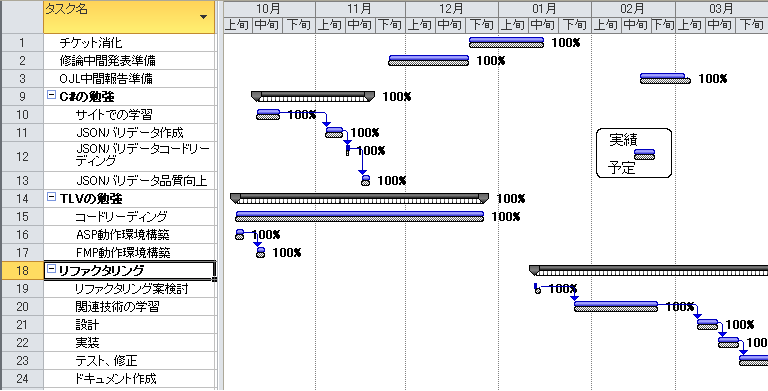
\includegraphics[width=\textwidth]{sch5.png}
\caption{�t�F�[�Y5�̃X�P�W���[��}\label{fig:sch5}
\end{figure}

\subsubsection{���{���e}
\begin{itemize}
\item �J���‹��̍\�z
\item JSON�o���f�[�^�̍쐬��ʂ���C\#��JSON�̊w�K
\item ���̍�Ƃ�ʂ���TLV�̊w�K
\begin{itemize}
\item TLV�̃R�[�h���[�f�B���O
\item TLV�̃}�j���A���ނ�ǂ�ŕs���_����Ȃǂ̃`�F�b�N
\end{itemize}
\item �s��Ɋւ���`�P�b�g�̒S��
\item ���t�@�N�^�����O�̌����Ǝ��{
\end{itemize}

\subsubsection{�X�P�W���[��} 
\figref{fig:sch5}�̂悤�ɁC��3��OJL�́C
2009�N10������J�n�����D�܂��CTLV�̊J���‹��𐮂�����C11�����܂�
TLV�Ƃ��̊J������ł���C\#�̊w�K���s�����DTLV��C\#�ɂ‚��Ă����悻��
�m�����‚����Ƃ���ŁC�s��Ɋւ���`�P�b�g��S�������D

1�����{�ɁCOJL2�����ɂ�郊�t�@�N�^�����O�Ẵ��r���[�ɎQ��������C
���t�@�N�^�����O��S�����邱�ƂɂȂ����D2�����܂Ŋ֘A�Z�p�ł���Parsec
�ƁC��������C�u�����Ƃ��Ă��ƒv���O���~���O����ł���Haskell�̊w�K��
�s�����D�Z�p�𗝉�������C���̋Z�p���Q�l�Ƀ��t�@�N�^�����O���s�����D

���ɖڗ������X�P�W���[���̒x���͂Ȃ������D

\subsubsection{����}
\ref{ch:refact}�͂ŏq�ׂ����t�@�N�^�����O���s�����D

�܂��CJSON�Ƃ��Đ������L�q����Ă��邩�`�F�b�N����JSON�o���f�[�^���쐬�����D
�w�K�̑��ɁC�ϊ����[���t�@�C���ƉŽ������[���t�@�C���p��JSON�o���f�[�^��
�쐬����ړI�����������C����ɂ‚��Ă͕ʂ�OJL3�������S�������D


\subsection{�t�F�[�Y6(2010�N�x�O��)}
\begin{figure}[!h]
\centering
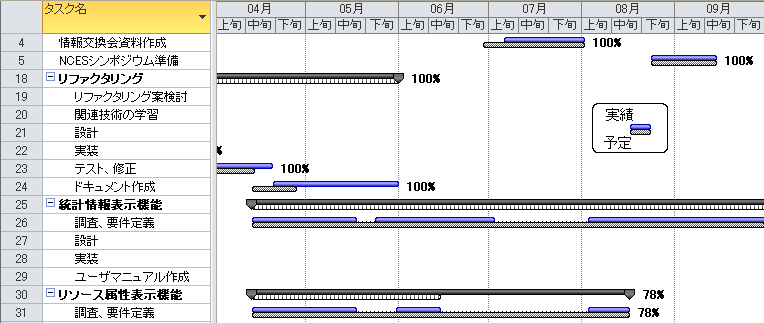
\includegraphics[width=\textwidth]{sch6.png}
\caption{�t�F�[�Y6�̃X�P�W���[��}\label{fig:sch6}
\end{figure}

\subsubsection{���{���e}
\begin{itemize}
\item ���t�@�N�^�����O��̃e�X�g�E�C���ƃh�L�������g�쐬
\item ���v���\���@�\�̎����”\�������Ɨv����`
\item ���\�[�X�����\���@�\�̎����”\�������Ɨv����`
\end{itemize}

\subsubsection{�X�P�W���[��} 
\figref{fig:sch6}�̂悤�ɁC�S�̓I��
�X�P�W���[���̒x�����ڗ������D

���t�@�N�^�����O�̃e�X�g�ƏC���ł̒x���́C�\��𗧂Ă�Ƃ�
�ɁC��r�̂��߂�C\#��Parsec����������TLV��p�ӂ��邱�Ƃ�z�肵�Ă���
���������Ƃɂ���D�܂��C�e�X�g���j���ł߂�̂Ɏ��Ԃ���������
���܂����̂������ł���D

�h�L�������g�̍쐬�ł̒x���ōl�����錴�������Ɏ����D
\begin{itemize}
\item �h�L�������g�̍쐬���j���쐬�r���ŕύX�ɂȂ�������
\item �M�҂̃h�L�������g�쐬�\�͂��Ⴂ����
\item ���v���\���@�\�ƃ��\�[�X�����\���@�\�̎����”\�������Ɠ����i
�s����������
\end{itemize}


���\�[�X�����\���@�\�Ƃ́C���\�[�X�̂��鎞���ɂ�����Z�}�t�H�Ȃǂ̑���
�̒l��\�`���ŕ\������@�\�ł���D���̋@�\�����[�U�̗v�]�Ƃ��ċ������Ă���D
���v���\���@�\�Ɠ��l�ɁC�Ž����\�����Ƃ͈قȂ�E�B���h�E�ɏ���\������
���̂�z�肵�Ă����̂ŁC�����”\�������𓝌v���\���@�\�Ɠ����i�s�����D

�����J�n�����CTLV�v���g�^�C�v�ɂ��̋@�\����������Ă����̂ŁC
���̖��c������Ɨ\�z�����D���̂��߁C�����������I��邾�낤�Ɣ��f���C���v
���\���@�\��葁����������\��ł������D�������CTLV�ɂ̓R�[�h�ȊO�̐�
�v�������R�����C�t�F�[�Y6�̎��_�ł�TLV�̐݌v�𗝉�������Ă��Ȃ������̂�
����C��������q�����D���̂��߁C���v���������C�����ɂ������”\������
���Ă��Ă������v���\���@�\�̎�����D�悳�����D

�����”\�������Ɨv����`��6�����Ƃ������ɑ����̎��Ԃ��������Ă��܂����D
����́C�v�����͂̎菇����@���K�؂ł͂Ȃ��������ƁC�K�؂Ȑ}��p���Ă���
���Ȃǂ̗��R�ōl�������܂�����ɓ`���Ȃ��������ƁC�z���葽���̗v����
�`������K�v�����������Ƃ��������ƍl����D

\subsubsection{����}
���t�@�N�^�����O�񍐏����쐬�����D


\subsection{�t�F�[�Y7(2010�N�x���)}
\begin{figure}[!h]
\centering
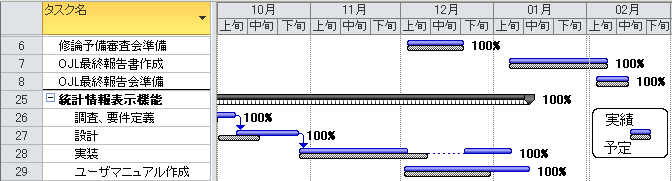
\includegraphics[width=\textwidth]{sch7.png}
\caption{�t�F�[�Y7�̃X�P�W���[��}\label{fig:sch7}
\end{figure}

\subsubsection{���{���e}
\begin{itemize}
\item ���v���\���@�\�̎����ƃ��[�U�}�j���A���쐬
\item .NET\ Framework\ 4�ւ̑Ή�
\item TLV���[�U1���ɂ�铝�v���\���@�\�̃��r���[
\end{itemize}

\subsubsection{�X�P�W���[��}
 \figref{fig:sch7}�̂悤�ɁC10������
���v���\���@�\�̐݌v�C�����ɒ��肵���D�\��ł́C12����
��{�Ŏ������Ђƒi������͂����������C.NET\ Framework\ 4�ւ�
�o�[�W�����A�b�v�ɂ��e�������E�΍�Ɏ��Ԃ����ꂽ��C
�f�o�b�O���Ɍ��‚���s��ɑΉ������肷�邱�ƂŒx�����������D

12������C���v���\���@�\��\sref{sec:sd_impl}�Ɏ��������̂�
�T�ˎ������I�����̂ŁC���[�U�}�j���A�����쐬���n�߂��D�܂��C
TLV���[�U1���ɋ��͂��Ē����C���v���\���@�\�̃��r���[�����{�����D

\subsubsection{����}
���v���\���@�\�����������D�܂��C���v���\���@�\�̃��[�U�}�j���A�����쐬�����D


\section{�`�P�b�g���̐���}
\begin{figure}[H]
\centering
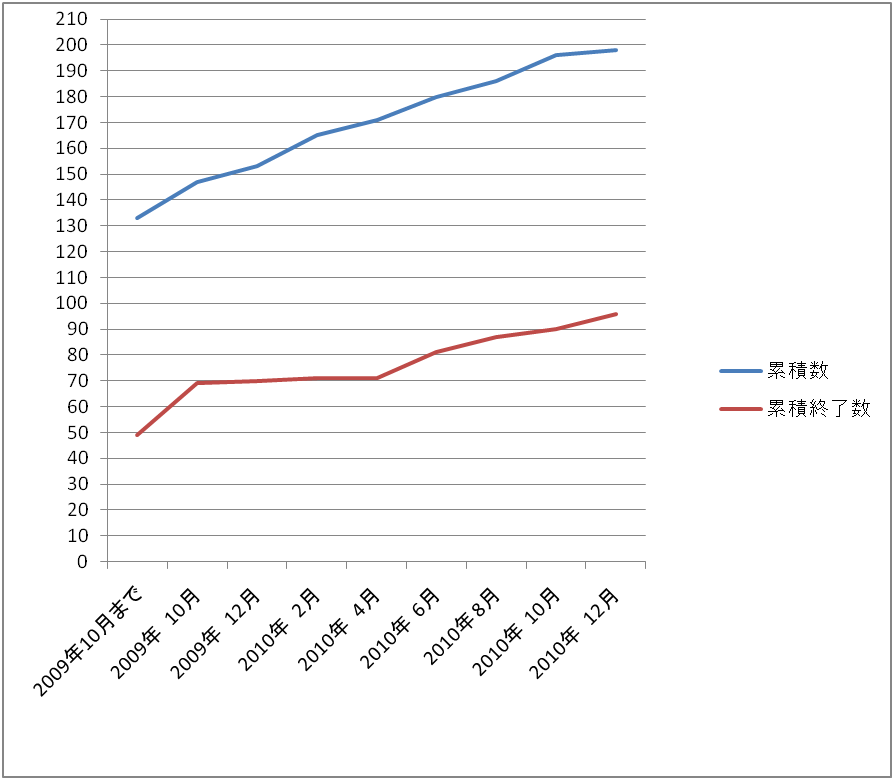
\includegraphics[width=\textwidth]{ticket.png}
\caption{�`�P�b�g�ݐό���}\label{ticket}
\end{figure}

��3��OJL�Ŏ��W�����v���E�s��͂��ׂ�Trac�̃`�P�b�g�Ƃ��ĊǗ������D
�t�F�[�Y5�ŐV��
�ɒlj����ꂽ�`�P�b�g������32���C�I�������`�P�b�g��22���C�t�F�[�Y6�ŐV��
�ɒlj����ꂽ�`�P�b�g������21���C�I�������`�P�b�g��16���C�t�F�[�Y7�ŐV��
�ɒlj����ꂽ�`�P�b�g������12���C�I�������`�P�b�g��9���ł������D

�`�P�b�g�̗ݐό����E�ݐϏI��������\figref{ticket}�Ɏ����D�}���C
�܂������i�K�ŁC���n�ɂ͂܂����Ԃ�v���邱�Ƃ��킩��D

\section{���\����}
2010�N9��15���ɍÂ��ꂽ��2��NCES�V���|�W�E��\footnote{http://www.nces.is.nagoya-u.ac.jp/news/sympo2010.html}�ɂă|�X�^�[���\���s�����D
\chapter{������}
\section{����}
OJL���o�����āC�傫��4�‚̂��Ƃ��w�K�����D

�܂��C�R�~���j�P�[�V�����̑�؂��C����ł���D���v���\���@�\�ɂ�����v����
�`�ŒɊ������D�v���𕪐͂���ہC������TLV���[�U�łȂ��C�܂��CRTOS�Ɋւ��錤����
�s���Ă����킯�ł��Ȃ��̂ŁC���v���ɂǂ̂悤�Ȃ��̂�����C�ǂ̂悤�ɂ���Γ�
����̂��C�ǂ̂悤�ɓ��v�������������̂��Ȃǂ킩��Ȃ������D�������C���[
�U�ɃA���P�[�g�Ƃ����`�ŃR�~���j�P�[�V��������邱�ƂŁC�v����`�̎������コ��
�邱�Ƃ��ł����D�܂��C���������╶���݂̂̃R�~���j�P�[�V�����́C�����̌����
�݁C�����̍l�������܂�����ɓ`�����Ȃ������D�}���g���ɂ��Ă��C�g�p����}���K
�؂��C�g�p���@�Ɍ�肪�Ȃ����ɋC��t���Ȃ���΁C����𐶂�ł��܂��D

���ɁC�h�L�������g�����̏d�v���ł���DTLV�̐݌v�E�����𒲍�����Ƃ��ɒɊ������DTLV�ɂ́C�N���X�}��V�[�P���X�}�Ȃǂ̐݌v�����Ȃ��C�\�[�X�R�[�h�ɂ��R�����g�����Ȃ��D���̂��߁C�e�N���X���ǂ̂悤�ɘA�g���C�N���X�̃����o�͂��ꂼ��ǂ̂悤�Ȗ���������̂����R�[�h���[�f�B���O�Ŕc������K�v������D���ʁC����������̒������ɂ‚Ȃ����Ă��܂����D

���ɁC�X�P�W���[���쐬�̓���ł���D�܂��C�\�t�g�E�F�A�J���o�����R�������߁C��Ƃ̐􂢏o��������ł���C���ς�����B���ł������D���̂��߁C�v��ʂ�ɂȂ��Ȃ��i�߂��Ȃ������D

�Ō�ɁC��Ɩڐ��ł̈ӌ���l�����Ȃǂɂӂ�‚�Ƃ��ł�����тł���D����́C
�ʏ�̍u�`�⌤���ł͖ő��ɖ��킦�Ȃ��̌��ł��邩�炾�D�ʏ�̍u�`�⌤���ł́C�w
�p�I�ȕ������傫�����C��Ƃ̖ڐ��́C��Ƃ̌�������v���W�F�N�g�Ǘ��̎�@�ȂǁC
���p�I�Ȃ��̂ł���悤�Ɋ������D

\section{�܂Ƃ�}
��3��OJL�ł́C�g���[�X���O�Ž����c�[���ł���TLV�̊J�����p�����čs���CTLV�ɑ΂�
�ē��v���\���@�\�̒lj��ƃg���[�X���O�p�[�T�̃��t�@�N�^�����O���s�����D�����
�́C���[�U������W�����v���̂����C���ɗv�������������uCPU���p���Ȃǂ̓��v����
�O���t�\���v�ƁuTLV�̍������v�ɑΉ��������̂ł���D

���v���\���@�\�̒lj��ɔ����C���v��񐶐����[���Ƃ����V�������[���𓱓������D����ɂ��C�g���[�X���O�₻��ȊO�̗l�X�ȃt�@�C�����瓝�v�����擾�E�������C���̓��v���ɓK�����O���t�̐ݒ肪�s����D�V�������[�������C�����̃��[���ɂ���\�������̃��[���ł��g�p����ꍇ�C�����̃��[���ɍ��킹�邱�Ƃŗ��p���@�̏K���̂��₷�������コ�����D�܂��C���v��񐶐����[���ɐ������[�h�Ƃ������v���̎擾�E�������郂�[�h��4��ޗp�ӂ��C���[�X�P�[�X�ɂ���Ďg����������悤�ɂ����D�\���Ɋւ��ẮC���v�����O���t�\������E�B���h�E��lj����C���v���̎擾�E�����ƃO���t�\����TLV���Ŋ��������C���̃A�v���P�[�V�����𗘗p�����ɍςނ悤�ɂ����D

�uTLV�̍������v���s�����߂ɂ́C�W���`���g���[�X���O�ւ̕ϊ��Ɛ}�`�f�[�^�̐���������������K�v������D���̍ہC���ꂼ��̏����Ɋւ���\�[�X�R�[�h�����G�����Ă���_����Q�ƂȂ�D�����ŁCOJL2�����ɂ���ė��Ă�ꂽ���t�@�N�^�����O���j���Q�l�ɁC�ϊ������Ɋ֌W����g���[�X���O�̃p�[�T�����̃��t�@�N�^�����O���s�����D���ʁC�p�[�T�E�R���r�l�[�^��p���邱�ƂŁC�R�[�h��EBNF��\���ł���悤�ɂȂ�C�“ǐ������サ�C�኱�Ȃ��獂�������}�ꂽ�D


\section{����̉ۑ�}
��3��OJL�Ŏ����������v���\���@�\�́C�\�z�E�݌v�i�K�ɂ����čl�����Ă��������‚��̋@�\���������؂�Ă��Ȃ��D�����̑Ή�����ȉۑ�ƂȂ�D�܂��C���v���\���@�\�ɑ΂��郆�[�U�̃��r���[�œ���ꂽ�A�C�f�B�A������C���v���\���@�\�͂܂����W�r��Ƃ�����D���݁C�m�F���Ă���ۑ���ȉ��Ɏ����D

\begin{itemize}
\item ���v��񐶐����[���t�@�C���̓��͂��Ž�����ɂ��s����@�\
\item ���ρE�ŏ��E�ő��\������O���t(���݁C�ςݏd�˃O���t���l���Ă���)
\item �O���t�\�����ɃO���t�ݒ��ύX�ł���u�O���t�ݒ�E�B���h�E�v�̎���
\item ��{��̓��[�h�ɂ�����u���肵���C�x���g�Ԋu�̃J�E���g�v���s����̓��\�b�h�̎���
\item ��{��̓��[�h�ɂ�����I�v�V�����ݒ�ł��鎖�O�����̐ݒ����
\item �Ž����\�����܂��̓}�N���r���[�A�Ŕ͈͎w�肵�������̓��v���𐶐����ăO���t�\������@�\
\item ���v��񓯎m�����Z�������ĐV���ȓ��v���𐶐�����@�\
\item �C�x���g�̎w���GUI�ōs����@�\(���v���\���@�\�̌���ł͂Ȃ�)
\end{itemize}


\chapter*{謝辞}
第3期OJLにおいて,多くのご指導を頂きました山本晋一郎教授
に深く感謝致します.
お忙しい中,副査を引き受けてくださった戸田尚宏教授,太田淳准教授
に深く感謝致します.

TLVを開発するにあたり,ご指導を頂きました名古屋大学大学院情報科学研究科
情報システム学専攻組込みリアルタイムシステム研究室の高田広章教授
に深く感謝致します.
また,開発プロジェクトマネージャとして
日頃より多くのご助言を頂きました
名古屋大学大学院情報科学研究科附属組込みシステム研究センターの
本田晋也准教授,
企業出身者としての立場から実践的なご意見を頂きました同研究センターの鴫原一人研究員,同研究センターの長尾卓哉研究員
に深く感謝致します.

統計情報表示機能に関して,アンケートにご協力下さいました名古屋大学大学院情報科学研究科附属込みシステム研究センターの松原豊研究員,同研究科情報システム学専攻組込みリアルタイムシステム研究室の安藤友樹氏
に深く感謝致します.また,統計情報表示機能のレビューにご協力下さいました同研究室の佐野泰正氏に深く感謝致します.

\begin{thebibliography}{99}%\addcontentlzissekiline{toc}{chapter}{\bibname}
\bibitem{goto} 後藤隼弐 『OJLによるトレースログ可視化ツールの開発』修士論文,名古屋大学,2009

\bibitem{ipsj}
後藤隼弐,
本田晋也,
長尾卓哉,
高田広章,トレースログ可視化ツールTraceLogVisualizer(TLV),コンピュータ ソフトウェア,Vol.27,No.4,pp.8-23,Nov 2010.

\bibitem{mz} 水野洋樹『トレースログ可視化ツール(TLV)に対する機能追加とリファクタリング』OJL報告書,
名古屋大学,2010

\bibitem{dm} 柳沢大祐『トレースログ可視化ツール(TLV)に対するアプリログ機能追加とプロファイリング』OJL報告書,
名古屋大学,2010

\bibitem{JSON}
RFC4627 The application/json Media Type for JavaScript Object Notation (JSON),http://tools.ietf.org/html/rfc4627,最終アクセス2011年2月1日

\bibitem{TOPPERS}
TOPPERS Project,http://www.toppers.jp/,最終アクセス2011年2月1日

\bibitem{itsp} OJL による最先端技術適応能力を持つIT 人材育成拠点
の形成,http://www.ocean.is.nagoya-u.ac.jp/,最終アクセス2011年2月1日

\bibitem{ojl} 小林隆志, 沢田篤史, 山本晋一郎, 野呂昌満, 阿草清滋, “On
the Job Learning: 産学連携による新しいソフトウェア
工学教育手法”,  電子情報通信学会信学技報SS2009-28,
vol.109, no.170, pp.95–100 2009

\bibitem{asp} TOPPERSプロジェクト/ASPカーネル,http://www.toppers.jp/asp-kernel.html,最終アクセス2011年2月1日

\bibitem{fmp} TOPPERSプロジェクト/FMPカーネル,http://www.toppers.jp/fmp-kernel.html,最終アクセス2011年2月1日

\bibitem{parsec}
LukeH's WebLog : Monadic Parser Combinators using C\# 3.0,\\
http://blogs.msdn.com/lukeh/archive/2007/08/19/monadic-parser-combinators-using-c-3-0.aspx\\
,最終アクセス2011年2月1日

\bibitem{msdn}
.NET Framework の正規表現,\\
http://msdn.microsoft.com/ja-jp/library/hs600312(v=VS.80).aspx
,最終アクセス2011年2月1日

\bibitem{msdncode}
グループ化構成体,\\
http://msdn.microsoft.com/ja-jp/library/bs2twtah\%28VS.80\%29.aspx\\
\#BalancingGroupDefinitionExample
,最終アクセス2011年2月1日



\end{thebibliography}
\end{document}

